\documentclass[9pt]{beamer}
\usepackage{amsmath, amssymb, amsthm, mathtools, graphicx, float, amssymb, subfigure, booktabs, enumitem}
\usepackage{hyperref}
\usepackage{enumitem}
\usepackage{minted}
\usepackage{pifont}
\usepackage{xcolor}
\usepackage[utf8]{inputenc} % usually not needed (loaded by default)
\usepackage[T1]{fontenc}
\hypersetup{colorlinks=true,citecolor=blue}
\usepackage{tikz}
\usepackage{fontawesome}
\usetikzlibrary{calc,shapes}
\usepackage[normalem]{ulem}
\setbeamertemplate{theorems}[numbered]
\usepackage[authoryear,round]{natbib}
\usepackage[portuguese]{babel}
\usetheme[pageofpages=of,% String used between the current page and the
                         % total page count.
          bullet=circle,% Use circles instead of squares for bullets.
          titleline=true,% Show a line below the frame title.
          alternativetitlepage=true,% Use the fancy title page.
          %titlepagelogo=logo-fiocruz,% Logo for the first page.
          %watermark=watermark-polito,% Watermark used in every page.
          %watermarkheight=100px,% Height of the watermark.
          %watermarkheightmult=4,% The watermark image is 4 times bigger
                                % than watermarkheight.
          ]{Torino}
\usecolortheme{chameleon}          
%%%% Box options
\newcommand{\tikzmark}[1]{\tikz[overlay,remember picture] \node (#1) {};}
%%%% Background settings          
% \setbeamercolor{normal text}{fg=white,bg=black!90}
% \setbeamercolor{structure}{fg=white}
% \setbeamercolor{alerted text}{fg=red!85!black}
% \setbeamercolor{item projected}{use=item,fg=black,bg=item.fg!95}
% \setbeamercolor*{palette primary}{use=structure,fg=structure.fg}
% \setbeamercolor*{palette secondary}{use=structure,fg=structure.fg!95!black}
% \setbeamercolor*{palette tertiary}{use=structure,fg=structure.fg!90!black}
% \setbeamercolor*{palette quaternary}{use=structure,fg=structure.fg!95!black,bg=black!80}
% \setbeamercolor{title}{fg=white}
% \setbeamercolor{frametitle}{bg=white}
% \setbeamercolor*{framesubtitle}{fg=white}
% \setbeamercolor*{block title}{parent=structure,bg=black!95}
% \setbeamercolor*{block body}{fg=black,bg=black!10}
% \setbeamercolor*{block title alerted}{parent=alerted text,bg=black!95}
% \setbeamercolor*{block title example}{parent=example text,bg=black!95}

%%%% Maths crap
\DeclareMathOperator*{\argmin}{arg\,min}
\DeclareMathOperator*{\argmax}{arg\,max}
\newtheorem{remark}{Remark}[]
\newtheorem{theo}{Teorema}[]
\newtheorem{exemplo}{Exemplo}
\newtheorem{defn}{Defini\c{c}\~ao}[]
\newtheorem{pergunta}{Pergunta}[]
\newtheorem{ideia}{Ideia}[]
\newtheorem{obs}{Observa\c{c}\~ao}[]
\newtheorem{property}{Property}[]
%%%% Itemize settings 
\setlist[itemize,1]{label=$\bullet$}
\setlist[itemize,2]{label=$\diamond$}

\setbeamercolor{block title}{use=structure,fg=white,bg=structure.fg!75!black}
\setbeamercolor{block body}{parent=normal text,use=block title,bg=block title.bg!10!bg}

%%%%%%%%%%%%%%%%%%%% Notation stuff
\newcommand{\indep}{\perp \!\!\! \perp} %% indepence
\newcommand{\pr}{\operatorname{Pr}} %% probability
\newcommand{\vr}{\operatorname{Var}} %% variance
\newcommand{\rs}{X_1, X_2, \ldots, X_n} %%  random sample
\newcommand{\irs}{X_1, X_2, \ldots} %% infinite random sample
\newcommand{\rsd}{x_1, x_2, \ldots, x_n} %%  random sample, realised
\newcommand{\Sm}{\bar{X}_n} %%  sample mean, random variable
\newcommand{\sm}{\bar{x}_n} %%  sample mean, realised
\newcommand{\Sv}{\bar{S}^2_n} %%  sample variance, random variable
\newcommand{\sv}{\bar{s}^2_n} %%  sample variance, realised
\newcommand{\bX}{\boldsymbol{X}} %%  random sample, contracted form (bold)
\newcommand{\bx}{\boldsymbol{x}} %%  random sample, realised, contracted form (bold)
\newcommand{\bT}{\boldsymbol{T}} %%  Statistic, vector form (bold)
\newcommand{\bt}{\boldsymbol{t}} %%  Statistic, realised, vector form (bold)
\newcommand{\emv}{\hat{\theta}_{\text{EMV}}}

\usepackage{url}
%%%% Hyperref stuff
\hypersetup{
  colorlinks  = true, %Colours links instead of ugly boxes
  urlcolor    = cyan, %Colour for external hyperlinks
  linkcolor   = cyan, %Colour of internal links
  citecolor   = red %Colour of citations
}
%%%% To create without the 'Figure' prefix. Remove if you need'em
\usepackage{caption}
\captionsetup[figure]{labelformat=empty}
%%%%
\author{
\underline{Luiz Max de Carvalho}[lmax.fgv@gmail.com]\linebreak
}
\title{
\Huge Inferência Estatística
}
\institute{
Disciplina da graduação em Matemática Aplicada\\
Escola de Matemática Aplicada (EMAp/FGV), Rio de Janeiro.
}
\date{\today}
\logo{\includegraphics[scale=.15]{logo.jpg}}
\begin{document}
% DO NOT COMPILE THIS FILE DIRECTLY!
% This is included by the other .tex files.
\section*{Primeira parte}
\begin{frame}[t,plain]
\titlepage
\end{frame}
%%%%%%%%%%%%%%%%%%%%%%%%%%%%%%%%%%%
%%%%%%%%%%%%%%%%%%%%%%%%%%%%%%%%%%%
\begin{frame}{Bem-vindas (os)!}
Este é um curso de 60 (sessenta) horas sobre Inferência Estatística.

\textbf{Princípios:}
\begin{itemize}
  \item[$\triangle$] Em uma palavra:~\underline{Liberdade};
  \item[$\triangle$] Construção conjunta do conhecimento;
  \item[$\triangle$] Pontualidade na entrega das tarefas;
  \item[$\triangle$] Participação em aula;
\end{itemize}

\textbf{Burocracia:}
\begin{itemize}
 \item[$\square$] Horário de atendimento: Segundas e quartas de 13:30h a 14:00h.
 \begin{itemize}
  \item  Por favor, mandar e-mail com antecedência de 24h para marcar;
  \end{itemize} 
 \item[$\square$] Podem escrever por e-mail (ou carta) quando quiserem;
 \item[$\square$] Teremos duas avaliações (A1 e A2) e 4 (quatro) trabalhos ($T_i$, $i = 1,2,3,4$).
 Trabalhos valerão 20\% do grau final.
 \item[$\square$] Sejam $N1 = A1 + T1 + T2$ e $N2 = A2 + T3 + T4$.
 
A \textbf{nota final} será $\text{NF} := (N_1 + N_2)/2$.
\end{itemize}
\end{frame}
%%%%%%%%%%%%%%%%%%%%%%%%%%%%%%%%%%%
%%%%%%%%%%%%%%%%%%%%%%%%%%%%%%%%%%%
\begin{frame}{Revisão de Teoria da Probabilidade}
\begin{itemize}
 \item Desigualdade de Markov;
 \item Desigualdade de Chebychev;
  \item Convergência;
 \item Lei(s) dos grandes números;
 \item Teorema(s) Central(is) do Limite;
\end{itemize}
\end{frame}
%%%%%%%%%%%%%%%%%%%%%%%%%%%%%%%%%%%
%%%%%%%%%%%%%%%%%%%%%%%%%%%%%%%%%%%
\begin{frame}{Desigualdade de Markov\footnote{Em homenagem a Andrey Andreyevich Markov (1856–1922).}}
\begin{theo}[Desigualdade de Markov]
 \label{them:Markov_ineq}
 Seja $X$ uma variável aleatória não-negativa e $t > 0$.
Então
\begin{equation}
 \label{eq:Markov_ineq}
 \pr(X \geq t) \leq \frac{E[X^n]}{t^n}.
\end{equation}
\end{theo}
\textbf{Prova:} Assumindo que $X$ é absolutamente contínua, escrever $E[X]$ explicitamente e usar linearidade e monotonicidade da integral.
Para $n = 1$ e $X$ discreta, ver DeGroot, página 349, Teorema 6.2.1 $\qed$
\end{frame}
%%%%%%%%%%%%%%%%%%%%%%%%%%%%%%%%%%%
\begin{frame}{Desigualdade de Chebychev\footnote{Em homenagem a Pafnuty Lvovich Chebyshev (1821--1894).}}
\begin{theo}[Desigualdade de Chebychev]
 \label{thm:Chebychev_ineq}
 Seja $Y$ uma variável aleatória com média $E[Y] =: \mu$ e variância $\vr(Y) =: \sigma^2$, ambas finitas.
Mais uma vez, $t>0$.
Então
\begin{equation}
 \label{eq:Chebychev_ineq}
 \pr(|Y-\mu| \geq t) \leq \frac{\vr(Y)}{t^2}.
\end{equation}
\end{theo}
\textbf{Prova:} Notar que $E[(Y-\mu)^2] = \sigma^2$ e aplicar Markov.
Ver DeGroot, página 349, Teorema 6.2.2 $\qed$
\end{frame}
%%%%%%%%%%%%%%%%%%%%%%%%%%%%%%%%%%%
\begin{frame}{A média amostral}
Considere uma~\textbf{amostra aleatória} $\rs$, $n \in \mathbb{N}$ de variáveis aleatórias de uma mesma distribuição com média $E[X_i] = \mu$ e variância $\vr(X_i) = \sigma^2$.
\begin{defn}[Média amostral]
 A média amostral de $\rs$ é
 \begin{equation}
  \label{eq:sample_mean}
  \bar{X}_n := \frac{1}{n} \sum_{i = 1}^n X_i.
 \end{equation}
\end{defn}

\begin{theo}[Média e variância em uma amostra i.i.d.]
\label{thm:iid_properties}
Sejam  $\rs$ variáveis aleatórias independentes e identicamente distribuídas, com média $\mu$ e variância $\sigma^2$.
Temos que (i) $E[\bar{X}_n] = \mu$ e (ii) $\vr(\bar{X}_n) = \frac{\sigma^2}{n}$.
\end{theo}
\textbf{Prova:} Para (i), usar a linearidade da esperança e o fato de as variáveis serem identicamente distribuídas -- note a falta de menção à independência.
Para (ii), usar a soma das variâncias de variáveis idependentes, além do fato de serem identicamente distribuídas.
Ver DeGroot, página 350, Teorema 6.2.3.
\end{frame}
%%%%%%%%%%%%%%%%%%%%%%%%%%%%%%%%%%%
\begin{frame}[allowframebreaks,fragile]{Exemplo: determinando o tamanho de amostra}
Vamos estudar o exemplo 6.2.3 de DeGroot.
Suponha  que uma moeda justa é lançada $n$ vezes.
Seja $X_i$ a variável aleatória que é $1$ se o $i$-ésimo lançamento dá cara e $0$ caso contrário.
Considere $\bar{X}_n = \frac{1}{n} \sum_{i=1}^n X_i$.
\begin{pergunta}[Quantos lançamentos?]
Quantos lançamentos devemos fazer para que 
$$ \pr(0.4 \leq \bar{X}_n \leq 0.6) \geq 0.7\: ?$$
\end{pergunta}
\textbf{Resolução:} Primeiro, faça $S_n = \sum_{i=1}^n X_i$ e deduza que $E[S_n] = np = n/2$ e $\vr(S_n) = n p(1-p) = n/4$.
Agora:
$$ \pr(0.4 \leq \bar{X}_n \leq 0.6) = \pr\left(\frac{4n}{10} \leq S_n  \leq \frac{6n}{10} \right).$$
Subtraia $E[S_n]$ dos dois lados da desigualdade para obter
$$ \pr\left(\frac{4n}{10} \leq S_n  \leq \frac{6n}{10} \right) = \pr \left(\left|S_n - \frac{n}{2} \right|\leq \frac{n}{10} \right) .$$
Note que, usando a desigualdade de Chebychev, temos uma cota superior para 
$$\pr \left(\left|S_n - \frac{n}{2} \right|\geq \frac{n}{10} \right) = 1 - \pr \left(\left|S_n - \frac{n}{2} \right|\leq \frac{n}{10} \right).$$
Portanto
$$\pr \left(\left|S_n - \frac{n}{2} \right|\geq \frac{n}{10} \right) \leq \frac{100}{4n}$$ 
e então
$$ \pr(0.4 \leq \bar{X}_n \leq 0.6) = \pr \left(\left|S_n - \frac{n}{2} \right|\leq \frac{n}{10} \right) \geq 1 - \frac{25}{n}.$$
Resolvendo $ 1 - 25/n = 0.7$ obtemos $n \geq 84$.

\framebreak
Agora, vamos usar o que sabemos~\textbf{especificamente} sobre este problema.
Usando uma tabela de probabilidades binomiais ou rodando um programa como:
\begin{minted}{R}
calcula_p <- function(n){
  prob <- pbinom(q = round(0.6*n), size = n, p = .5) 
  - pbinom(q = round(0.4*n)-1, size = n, p = .5)
  return(prob)
}
n <- 10
p <- calcula_p(n)
alvo <- 0.7
erro <- (p-alvo)^2
while(erro > .001){
  n <- n + 1
  p <- calcula_p(n)
  erro <- (p-alvo)^2
  if(n > 10000) break
}
\end{minted}
obtemos \verb|n = 15| e \verb|p = 0.6982422|.

\textbf{Conclusão}: a desigualdade de Chebychev é~\underline{frouxa}, isto é, ela dá uma cota superior para a probabilidade de interesse, mas essa cota pode ser muito maior do que o valor exato.
Por outro lado, a desigualdade é válida para~\underline{qualquer} variável aleatória cuja variância exista e seja finita.

\begin{ideia}[Sem almoço grátis]
\label{idea:no_free_lunch}
 Se uma técnica ou resultado é muito geral, isto é, se aplica a muitas situações, há grandes chances de não fornecer uma resposta muito precisa.
 O contrário também é verdadeiro: se desenvolvemos uma técnica elaborada para uma classe restrita de problemas, geralmente vamos obter respostas precisas, mas nossa técnica não será aplicável a muitos tipos de problemas.
 Em Estatística não existe almoço grátis.
\end{ideia}

\end{frame}
%%%%%%%%%%%%%%%%%%%%%%%%%%%%%%%%%%%
\begin{frame}{Convergência}
\begin{defn}[Convergência em probabilidade]
\label{defn:weak_convergence}
Dizemos que uma sequência de variáveis aleatórias~\textit{converge em probabilidade} para $b$ se, para todo $\epsilon > 0$, temos
\begin{equation}
 \nonumber
 \lim_{n\to\infty} \pr\left(|Z_n-b| < \epsilon \right) = 1.
\end{equation}
Neste caso, escrevemos $Z_n \xrightarrow{\text{p}} b$.
\end{defn}
Em algumas situações, chamamos a convergência em probabilidade de convergência fraca.
\end{frame}
%%%%%%%%%%%%%%%%%%%%%%%%%%%%%%%%%%%
\begin{frame}{Lei(s) dos Grandes Números (LGN)}
A lei fraca dos grandes números é um resultado fundamental da Teoria de Probabilidade, extremamente útil em Estatística.
\begin{theo}[Lei Fraca dos Grandes Números]
\label{thm:WLLN}
Sejam  $\rs$ variáveis aleatórias independentes e identicamente distribuídas, com média $\mu$ e variância $\sigma^2$.
 Então
 $$ \bar{X}_n \xrightarrow{\text{p}} \mu.$$
\end{theo}
\textbf{Prova:}
Usando o teorema~\ref{thm:iid_properties} e a desigualdade de Chebychev, temos
$$ \pr\left( |\bar{X}_n - \mu| < \epsilon\right) \geq  1 - \frac{\sigma^2}{n\epsilon^2},$$
e, portanto,
$$ \lim_{n\to\infty} \pr\left( |\bar{X}_n - \mu| < \epsilon\right) = 1. \: \qed$$
\end{frame}
%%%%%%%%%%%%%%%%%%%%%%%%%%%%%%%%%%%
\begin{frame}{LGN: exemplo}
$X_1, \ldots, X_n \sim \operatorname{Beta}(3, 2)$.
$E[X] = \alpha / (\alpha + \beta) = 3/5$.
\begin{figure}[!ht]
\label{fig:beta_LGN}
\begin{center}
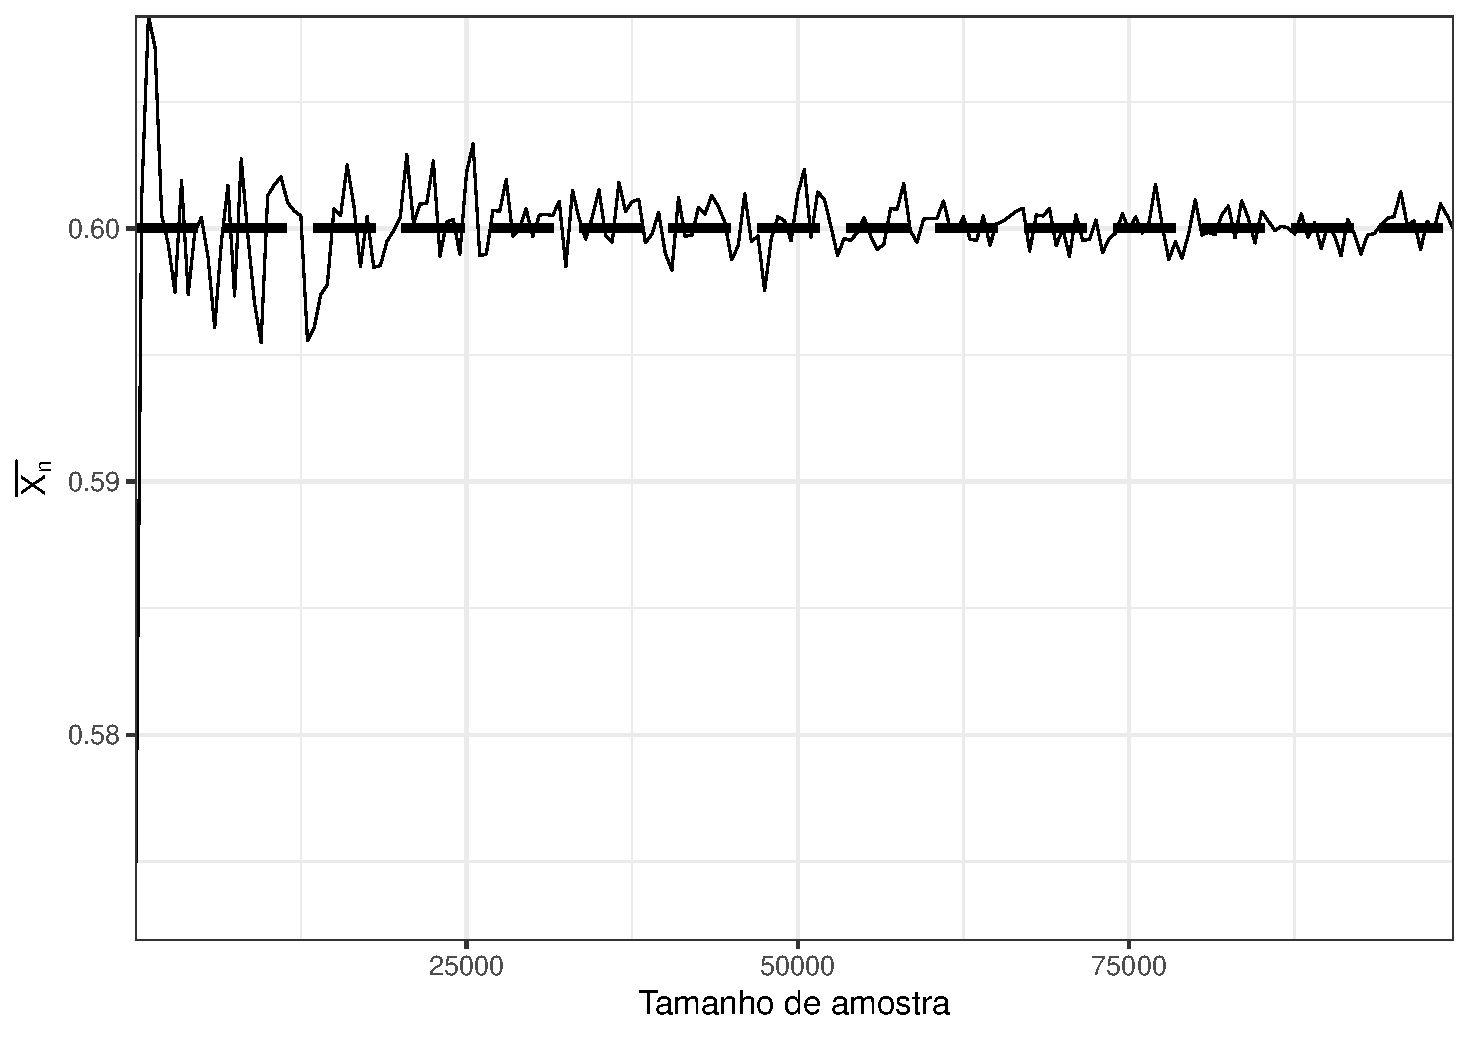
\includegraphics[scale=0.35]{figures/beta_3_2_LGN.pdf} 
\end{center} 
\end{figure} 
\end{frame}
%%%%%%%%%%%%%%%%%%%%%%%%%%%%%%%%%%%
\begin{frame}{Comentário: Lei Forte dos Grandes Números}
\begin{defn}[Convergência quase certa]
 \label{dfn:as_convergence}
Dizemos que uma sequência de variáveis aleatórias $\left(Z_n\right)_{n\geq 1}$~\textit{converge quase certamente} para $b$ se
$$\pr\left(\lim_{n\to \infty} Z_n = b\right) = 1.$$
\end{defn}
Esse modo de convergência é por vezes chamado de convergência forte.
\textbf{Observação}: convergência quase certa implica convergência em probabilidade.
 \begin{theo}[\textbf{Lei forte dos grandes números}]
  \label{thm:SLLN}
   Sejam  $X_1, X_2, \ldots $ variáveis aleatórias independentes e identicamente distribuídas, com média $\mu$.
 Então
 $$\pr\left(\lim_{n\to \infty} \bar{X}_n = \mu \right) = 1.$$
 \end{theo}
\end{frame}
%%%%%%%%%%%%%%%%%%%%%%%%%%%%%%%%%%%
\begin{frame}[fragile]{Teorema(s) Central(is) do Limite}
O Teorema Central do Limite um dos resultados mais importantes da Estatística.
\begin{theo}[Teorema Central do Limite (Lindeberg e Lévy)\footnote{Jarl Waldemar Lindeberg (1876--1932) e Paul Pierre Lévy (1886--1971).}]
 \label{thm:CLT_LindebergLevy}
Sejam  $\rs$ variáveis aleatórias independentes e identicamente distribuídas, com média $\mu$ e variância $\sigma^2$.
Então, para cada $x$, temos
$$ \lim_{n\to\infty} \pr\left( \frac{\bar{X}_n - \mu}{\sigma/\sqrt{n}} \leq x \right) = \Phi(x), $$
onde 
$$\Phi(x) := \frac{1}{\sqrt{2\pi}}\int_0^x \exp\left(-\frac{t^2}{2}\right)dt,$$
é a função de distribuição (cumulativa) normal padrão.
\end{theo}
\textbf{Prova}: Ver Casella \& Berger (2002), página 237, teorema 5.5.14.
% Assuma que a função geradora de momentos, $M_X(t)$, existe na vizinhança de zero -- i.e. para $|t| < h, h > 0$.
% 
\end{frame}
%%%%%%%%%%%%%%%%%%%%%%%%%%%%%%%%%%%
\begin{frame}{Teorema Central do Limite: interpretação}
\begin{itemize}
 \item Sabemos que a variável aleatória padronizada $Y_n := \left(\bar{X}_n - \mu\right)/\sigma$ tem média 0 e variância 1, por construção;
 \item O teorema~\ref{thm:CLT_LindebergLevy} nos diz que se tomamos uma amostra grande de uma distribuição com média $\mu$ e variância $\sigma^2$, a variável aleatória $\sqrt{n}Y_n$ terá, aproximadamente, distribuição~\textbf{normal} com média 0 e desvio padrão $1$, chamada~\textit{distribuição normal padrão};
 \item Isto equivale a dizer que $\bar{X}_n \sim \operatorname{normal}(\mu, \sigma^2/n)$;
 \item Note que o teorema vale para~\underline{qualquer} variável aleatória cujos dois primeiros momentos existam, seja ela discreta ou contínua!
\end{itemize}
\end{frame}
%%%%%%%%%%%%%%%%%%%%%%%%%%%%%%%%%%%
\begin{frame}{Teorema Central do Limite: aplicação}
\begin{pergunta}[Quanto vale $p$?]
Suponha que $X_1, \ldots, X_{12}$ são variáveis aleatórias independentes com distribuição uniforme entre 0 e 1.
Defina
$$  p:=  \pr\left(\left| \bar{X}_n - \frac{1}{2}\right| \leq 0.1\right).$$
Quanto vale $p$?
\end{pergunta}
\textbf{Resolução}: 
Lembremos que a variável padronizada $Z = \sqrt{n}(\bar{X}_n-E[X])/\sqrt{\vr(X)}$ terá distribuição aproximadamente normal padrão.
Se $X\sim \operatorname{uniforme}(0, 1)$, sabemos que $E[X] = 1/2$ e $\vr(X) = 1/12$.
Nos aproveitando do fato de que $\sqrt{n}$ e $\sigma$ coincidem nesse exemplo, escrevemos
$$\pr\left(\left| \bar{X}_n - \frac{1}{2}\right| \leq 0.1\right) =  \pr\left(12\left| \bar{X}_n - \frac{1}{2}\right| \leq 0.1\times 12\right) = \pr(|Z| < 1.2),$$
de modo que $p \approx \Phi(1.2)-\Phi(-1.2) = 0.7698607$.
O valor exato, que não discutiremos como obter, é $p = 0.7667213$.
% \footnote{Chebychev diz que $p \geq 1 - 1/(144 \times 0.1^2) \approx 0.31$, o que está longe do valor exato.}
\end{frame}
%%%%%%%%%%%%%%%%%%%%%%%%%%%%%%%%%%%
\begin{frame}{O que aprendemos?}
\begin{itemize}
\item[\faLightbulbO] Desigualdades de Markov e Chebychev: extremamente gerais (mas não muito precisas!);
\item[\faLightbulbO] Convergência fraca (convergência em probabilidade ou medida), $Z \xrightarrow{\text{p}} b$;
\item[\faLightbulbO] Lei (fraca) dos grandes números: a média amostral converge para a média populacional à medida que a amostra aumenta, $\bar{X}_n \xrightarrow{\text{p}} \mu$;
\item[\faLightbulbO] Teorema Central do Limite: para amostras grandes o suficiente, 
$$\bar{X}_n \sim \operatorname{normal}(\mu, \sigma^2/n).$$
\end{itemize} 
\end{frame}
%%%%%%%%%%%%%%%%%%%%%%%%%%%%%%%%%%%
\begin{frame}{Leitura recomendada}
\begin{itemize}
 \item[\faBook] DeGroot seções 6.2 e 6.3;
 \item[\faBook] $^\ast$ Casella \& Berger, seções 5.2 e 5.5;
 \item[‡\faGithub] $^\ast$ Nosso repositório (\url{https://github.com/maxbiostat/Statistical_Inference_BSc}).
  \item[\faForward] Próxima aula: DeGroot, seção 7.1;
  \end{itemize} 
\end{frame}

% DO NOT COMPILE THIS FILE DIRECTLY!
% This is included by the other .tex files.
\section*{Inferência Estatística}
%%%%%%%%%%%%%%%%%%%%%%%%%%%%%%%%%%%
%%%%%%%%%%%%%%%%%%%%%%%%%%%%%%%%%%%
\begin{frame}{O que é e para que serve Inferência Estatística?}

\begin{itemize}
 \item[\faQuestion] Esta moeda é justa?
 \item[\faQuestion] Esta droga ``funciona''?
 \item[\faQuestion] Quantos casos de Dengue teremos mês que vem?
 \item[\faQuestion] Renda básica universal aumenta o PIB?
\end{itemize}

Todas essas perguntas podem ser abordadas com as ferramentas que a Estatística nos fornece.

\begin{ideia}
\textbf{A Estatística é a gramática da Ciência}\footnote{Título do livro de Karl Pearson (1857--1936) (\href{https://en.wikipedia.org/wiki/The_Grammar_of_Science}{``The Grammar of Science''}), publicado em 1982.}.
O mundo é incerto; medições são imperfeitas.
A Estatística é a linguagem que nos permite expressar e quantificar as incertezas associadas às afirmações científicas através da teoria de probabilidades\footnote{Chamada por E.T. Jaynes (1922-1998) de lógica da Ciência (\href{https://www.cambridge.org/gb/academic/subjects/physics/theoretical-physics-and-mathematical-physics/probability-theory-logic-science}{``Probability Theory: The Logic of Science''}).}.
\end{ideia}
\end{frame}
%%%%%%%%%%%%%%%%%%%%%%%%%%%%%%%%%%%
\begin{frame}{Modelo estatístico: definição informal}
\begin{defn}
  \textbf{Modelo estatístico} (De Groot, def 7.1.1, pág. 377).  
Um modelo estatístico consiste na identificação de variáveis aleatórias de interesse (observáveis e potencialmente observáveis), na especificação de uma distribuição conjunta para as variáveis aleatórias observáveis e na identificação dos parâmetros ($\theta$) desta distribuição conjunta.
Às vezes é conveniente assumir que os parâmetros são variáveis aleatórias também, mas para isso é preciso especificar uma distribuição conjunta para $\theta$.
\end{defn}
 
\end{frame}
%%%%%%%%%%%%%%%%%%%%%%%%%%%%%%%%%%%
\begin{frame}{Modelo estatístico: definição formal}
\begin{defn}
 \textbf{Modelo estatístico} (\href{https://projecteuclid.org/download/pdf_1/euclid.aos/1035844977}{McCullagh, 2002}).
 Seja $\mathcal{X}$ um espaço amostral qualquer, $\Theta$ um conjunto não-vazio arbitrário e $\mathcal{P}(\mathcal{X})$ o conjunto de todas as distribuições de probabilidade em $\mathcal{X}$.
 Um modelo estatístico~\underline{paramétrico} é uma função $P : \Theta \to \mathcal{P}(\mathcal{X})$, que associa a cada $\theta \in \Theta$ uma distribuição de probabilidade $P_\theta$ em $\mathcal{X}$.
\end{defn}
\textbf{Exemplos}:
\begin{itemize}
 \item Faça $\mathcal{X} = \mathbb{R}$ e $\Theta = (-\infty, \infty)\times (0, \infty)$.
 Dizemos que $P$ é um modelo\footnote{Note o abuso de notação: estritamente falando, $P_\theta$  é uma~\textbf{medida} de probabilidade e não uma~\textit{densidade} como apresentamos aqui.} estatístico normal se para cada $\theta = \{\mu, \sigma^2\} \in \Theta$,
 $$P_{\theta}(x) \equiv \frac{1}{\sqrt{2\pi}\sigma}\exp\left(-\frac{(x-\mu)^2}{2\sigma^2}\right), \: x \in \mathbb{R}.$$
 \item Faça $\mathcal{X} = \mathbb{N}\cup \{0\}$ e $\Theta = (0, \infty)$.
 $P$ é um modelo estatístico Poisson se para $\lambda \in \Theta$,
 $$P_{\lambda}(k) \equiv \frac{e^{-\lambda}\lambda^k}{k!}, \: k = 0, 1, \ldots$$
\end{itemize} 
\end{frame}

%%%%%%%%%%%%%%%%%%%%%%%%%%%%%%%%%%%
\begin{frame}{Exemplo: como sempre, moedas.}
 \begin{pergunta}[Esta moeda é justa?]
 \label{ex:moeda_justa}
  Suponha que uma moeda tenha sido lançada dez vezes, obtendo o seguinte resultado:
  \begin{equation*}
   KKKCKCCCKC
  \end{equation*}
\begin{itemize}
 \item[a)] Esta moeda é justa?
 \item[b)] Quanto eu espero ganhar se apostar R\$ 100,00 que é justa? 
\end{itemize}
 \end{pergunta}
 Podemos formalizar o problema ao, por exemplo, assumir que cada lançamento é uma variável aleatória Bernoulli com probabilidade de cara ($K$), $p$.
 Desta forma $X_i = 1$ se o lançamento deu cara e $X_i = 0$ caso contrário.
 E queremos saber se $p = 1/2$.
 Por ora, não temos as ferramentas necessárias para responder a essa pergunta, mas voltaremos a ela no futuro.
\end{frame}
%%%%%%%%%%%%%%%%%%%%%%%%%%%%%%%%%%%
\begin{frame}{Inferência Estatística}
\begin{defn}
 \textbf{Afirmação probabilística}.
 Dizemos que uma afirmação é probabilística quando ela utiliza conceitos da teoria de probabilidade para falar de um objeto.
 Exemplos: 
 \begin{itemize}
  \item $\pr( \bar{Y}_n \in (0, 1)) \leq 2^{-n}$;
  \item $E[X \mid Y = y] = 2y + 3$;
  \item $\vr(X) = 4p^2$.
  \item $\pr(\vr(X) \leq 4p^2 ) \leq p^2$
 \end{itemize}
\end{defn}
\begin{defn}
 \textbf{Inferência Estatística}.
 Uma inferência estatística é uma~\underline{afirmação probabilística} sobre uma ou mais partes de um modelo estatístico.
 Considerando o exemplo~\ref{ex:moeda_justa}, queremos saber:
 \begin{itemize}
  \item Quantos lançamentos até termos $80\%$ de certeza de que a moeda é justa?
%   \item Se $p$ é a probabilidade de obter cara num dado lançamento e $\hat{p}$ é nossa estimativa para $p$, quanto vale $E[\hat{p}]$? E $\vr(\hat{p})$?
  \item Quanto vale $E[\bar{X}_n]$;
  \item $\pr(X_{n} = 1 \mid X_{n-1} = 1)$. 
 \end{itemize}
\end{defn}
\end{frame}
%%%%%%%%%%%%%%%%%%%%%%%%%%%%%%%%%
\begin{frame}{Estatística}
\begin{defn}
 \textbf{Estatística}.
 Suponha que temos uma coleção de variáveis aleatórias $\rs \in \boldsymbol X \subseteq \mathbb{R}^n$ e uma função $r: \boldsymbol X \to \mathbb{R}^m$.
 Dizemos que a variável aleatória $T = r(\rs)$ é uma~\textbf{estatística}.
\end{defn}
São exemplos de estatísticas:
\begin{itemize}
 \item A média amostral, $\bar{X}_n$;
 \item A soma, $\sum_{i=1}^n X_i$;
 \item O mínimo, $\min(\rs)$;
 \item $r(\rs) = a, \: \forall \rs, \: \, a \in \mathbb{R}$.
\end{itemize}  
\end{frame}
%%%%%%%%%%%%%%%%%%%%%%%%%%%%%%%%%
\begin{frame}{Tipos de Inferência Estatística}
\begin{itemize}
 \item \textbf{Predição}: prever o valor de uma variável aleatória (ainda) não observada; No exemplo~\ref{ex:moeda_justa}, qual será o valor do próximo lançamento, $X_{n+1}$;
 \item \textbf{Decisão Estatística}: Acoplamos o modelo estatístico a uma decisão a ser tomada. Devo emprestar esta moeda ao Duas-Caras? Aqui, temos a~\textit{noção} de~\textbf{risco}.;
 \item \textbf{Desenho experimental}: Quantas vezes é preciso lançar esta moeda para ter 95\% de certeza de que ela é (ou não) justa? Quantas pessoas precisam tomar uma droga para sabermos se ela funciona? Onde devemos cavar para procurar ouro/petróleo?;
\end{itemize}
\end{frame}
%%%%%%%%%%%%%%%%%%%%%%%%%%%%%%%%%
\begin{frame}{O que aprendemos?}
\begin{itemize}
 \item[\faLightbulbO] Modelo estatístico;
 \item[\faLightbulbO] Inferência Estatística;
 \item[\faLightbulbO] Estatística (amostral);
 \item[\faLightbulbO] Tipos de inferências:
 \begin{itemize}
  \item Predição;
  \item Decisão;
  \item Desenho experimental.
 \end{itemize}
%  \item[\faLightbulbO] Estimador:
\end{itemize}
\end{frame}
%%%%%%%%%%%%%%%%%%%%%%%%%%%%%%%%%
\begin{frame}{Leitura recomendada}
\begin{itemize}
 \item[\faBook] De Groot seção 7.1;
 \item[\faFilePdfO] $^\ast$ \href{https://projecteuclid.org/download/pdf_1/euclid.aos/1035844977}{McCullagh, 2002}.
\end{itemize} 
\end{frame}
%%%%%%%%%%%%%%%%%%%%%%%%%%%%%%%%%

% DO NOT COMPILE THIS FILE DIRECTLY!
% This is included by the other .tex files.
\section*{Estimadores bayesianos}
\begin{frame}{Estatística bayesiana}
 \begin{itemize}
  \item Os paradigmas bayesiano e frequentista; 
  \item Distribuição~\textit{a priori} e~\textit{a posteriori};
%   \item Sensibilidade e prioris impróprias;
  \item Função de verossimilhança;
  \end{itemize}  
  \begin{columns}
    \begin{column}{0.5\textwidth}
        \begin{figure}[!ht]
        \label{fig:bayes_sign}
        \begin{center}
        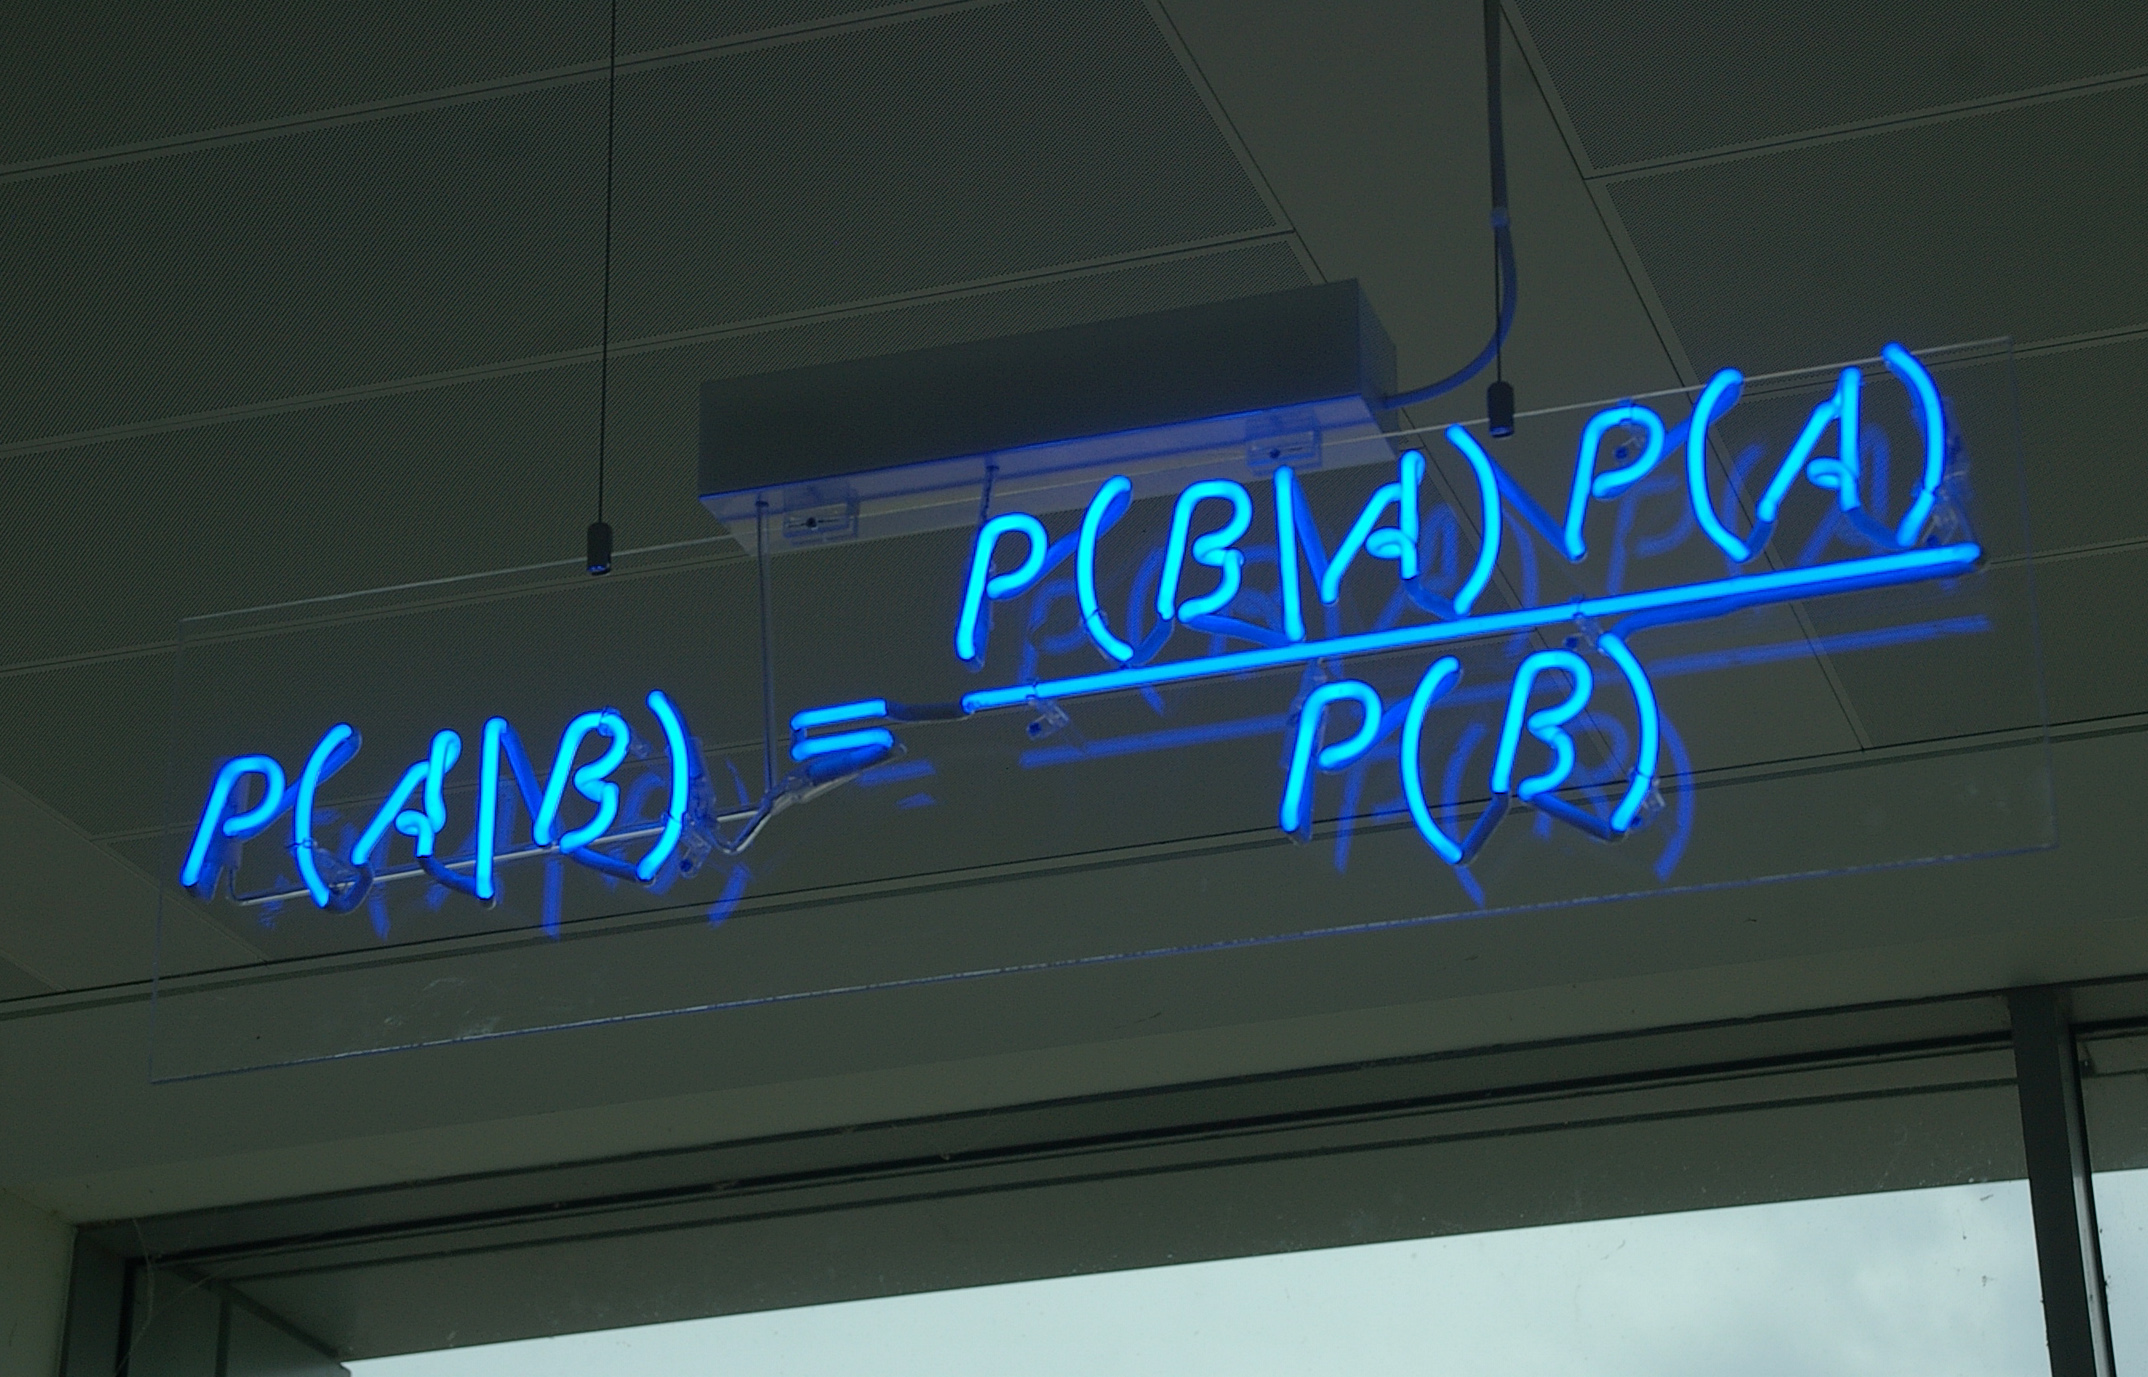
\includegraphics[scale=0.07]{figures/Bayes_Theorem_MMB_01.jpg} 
        \end{center}
        \end{figure}        
    \end{column}
\begin{column}{0.5\textwidth}
   \begin{figure}[!ht]
    \label{fig:bayes_graph}
    \begin{center}
    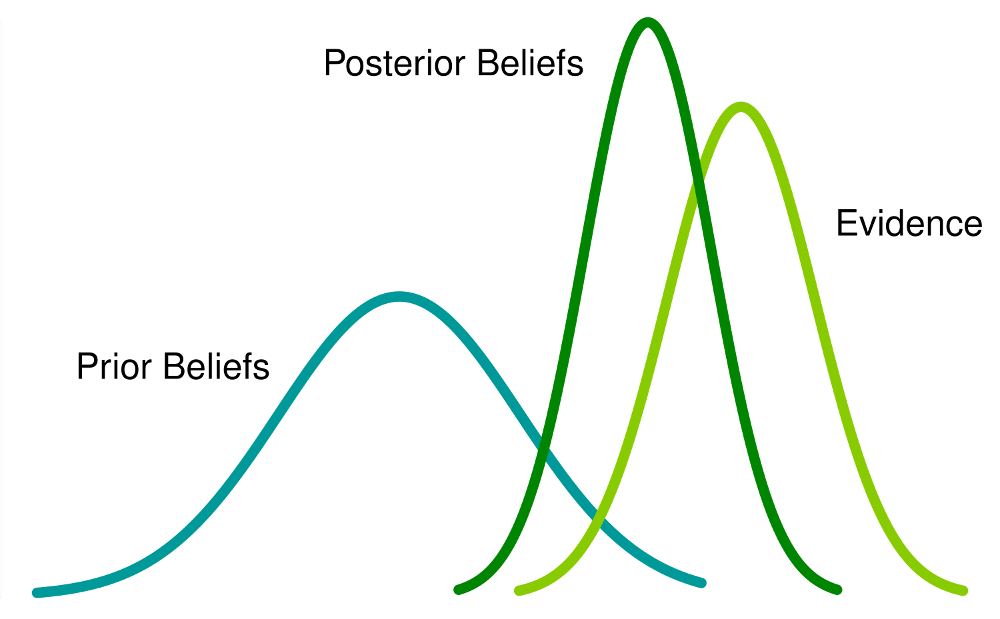
\includegraphics[scale=1.0]{figures/bayesian_inference.jpg} 
    \end{center} 
    \end{figure} 
\end{column}
  \end{columns}  
\end{frame}
%%%%%%%%%%%%%%%%%%%%%%%%%%%%%%%%%%%
\begin{frame}{Permutabilidade}
\begin{defn}
\label{def:exchangeability}
 \textbf{Permutabilidade}.
 Uma coleção finita de variáveis aleatórias $\rs$ com densidade conjunta $f$ é dita~\textbf{permutável} se 
 \[f(x_1, x_2, \ldots, x_n) = f( x_{\pi(1)}, x_{\pi(2)}, \ldots, x_{\pi(n)} ), \]
 para qualquer permutação $\boldsymbol\pi = \{\pi(1), \pi(2), \ldots, \pi(n)\}$ dos seus elementos.
 Uma coleção infinita é permutável se qualquer subconjunto finito é permutável.
\end{defn}
\begin{itemize}
 \item Note que uma amostra permutável não precisa ser independente;
 \item Note também que IID $\implies$ permutável;
 \item A intuição é simples: simetria.
\end{itemize}
\end{frame}
%%%%%%%%%%%%%%%%%%%%%%%%%%%%%%%%%%%
\begin{frame}{Parâmetros como limites de variáveis aleatórias.}
\begin{exemplo}
\label{ex:remission}
 \textbf{Ensaio Clínico (De Groot, exemplo 7.1.3).}
 Suponha que estamos interessados na taxa de recrudescência (``recaída'') de uma determinada doença entre pacientes tratados com uma droga.
 Seja $X_i$ a variável aleatória que indica se o $i$-ésimo paciente recrudesceu ($X_i = 1$) ou não ($X_i = 0$).
 Seja $P$ a proporção de indivíduos que recrudescem num grupo grande de pacientes. 
 Se $P$ é desconhecida, podemos modelar $\irs$ como variáveis aleatórias Bernoulli IID com parâmetro $p$~\textbf{condicional} a $P = p$.
 Em notação estatística:
 \[ \irs \mid P = p \sim \operatorname{Bernoulli}(p).\]
  \textbf{Assuma} que $\irs$ é uma sequência permutável infinita.
  Agora chamemos de $P_n$ a proporção de pacientes que recrudescem nos $n$ primeiros pacientes.
  Podemos mostrar que o limite $\lim_{n \to \infty} P_n = \lim_{n \to \infty} \sum_{i=1}^n X_i/n$ existe com probabilidade 1 e que pode ser visto como a proporção $P$.
\end{exemplo}
\end{frame}
%%%%%%%%%%%%%%%%%%%%%%%%%%%%%%%%%%%
\begin{frame}{Paradigmas de inferência}
No Exemplo~\ref{ex:remission} podemos encarar o problema de duas maneiras:
\begin{itemize}
 \item[A)] $P$ é uma variável aleatória e $\irs$ são $\operatorname{Bernoulli}(p)$~\textbf{condicional} ao evento $P = p$, $p \in (0, 1)$.
 \item[B)] Para uma constante fixa (e inobservável) $p$, $\irs$ tem distribuição $\operatorname{Bernoulli}$ com parâmetro $p$ -- isto é, indexada por $p \in (0, 1)$.
\end{itemize}
Uma diferença~\textit{sutil}, não é?
A tradição estatística que entende parâmetros como variáveis aleatórias como em A) é chamada de \textbf{Estatística bayesiana}\footnote{Em homenagem ao reverendo inglês Thomas Bayes (1701 -- 1761).}.
Já os que aderem à abordagem B) são chamados~\textbf{frequentistas} -- ou ortodoxos, como Jaynes gosta de chamá-los.
Neste curso veremos conceitos e exemplos destas duas escolas de pensamento. 
\end{frame}
%%%%%%%%%%%%%%%%%%%%%%%%%%%%%%%%%%%
\begin{frame}{Uma análise bayesiana}
\begin{exemplo}
\label{ex:duracao_componentes}
\textbf{Duração de componentes eletrônicos (De Groot, exemplo 7.2.1).}
Suponha que uma empresa esteja interessadas em saber o quanto duram os produtos que ela produz.
Se representamos os tempos de duração de $n$ objetos como $n$ variáveis aleatórias $\rs$ IID com distribuição exponencial com parâmetro $\theta$ de modo que
$$f(x_i \mid \theta) = \theta \exp(-\theta x_i), x_i > 0.$$
\textbf{Observação:} $n/\sum_{i=1}^n \xrightarrow{\text{p}} \theta$.

Aqui, $\theta$ é a taxa de falha dos componentes, e é um parâmetro de interesse.
Suponha que uma pessoa experiente na empresa diga que a taxa de falha é mais ou menos $0.5$/ano.
Como representamos esta informação?
\end{exemplo} 
\end{frame}
%%%%%%%%%%%%%%%%%%%%%%%%%%%%%%%%%%%
\begin{frame}{Uma análise bayesiana (cont.)}
 \begin{figure}[!ht]
\label{fig:gamma_1_2}
\begin{center}
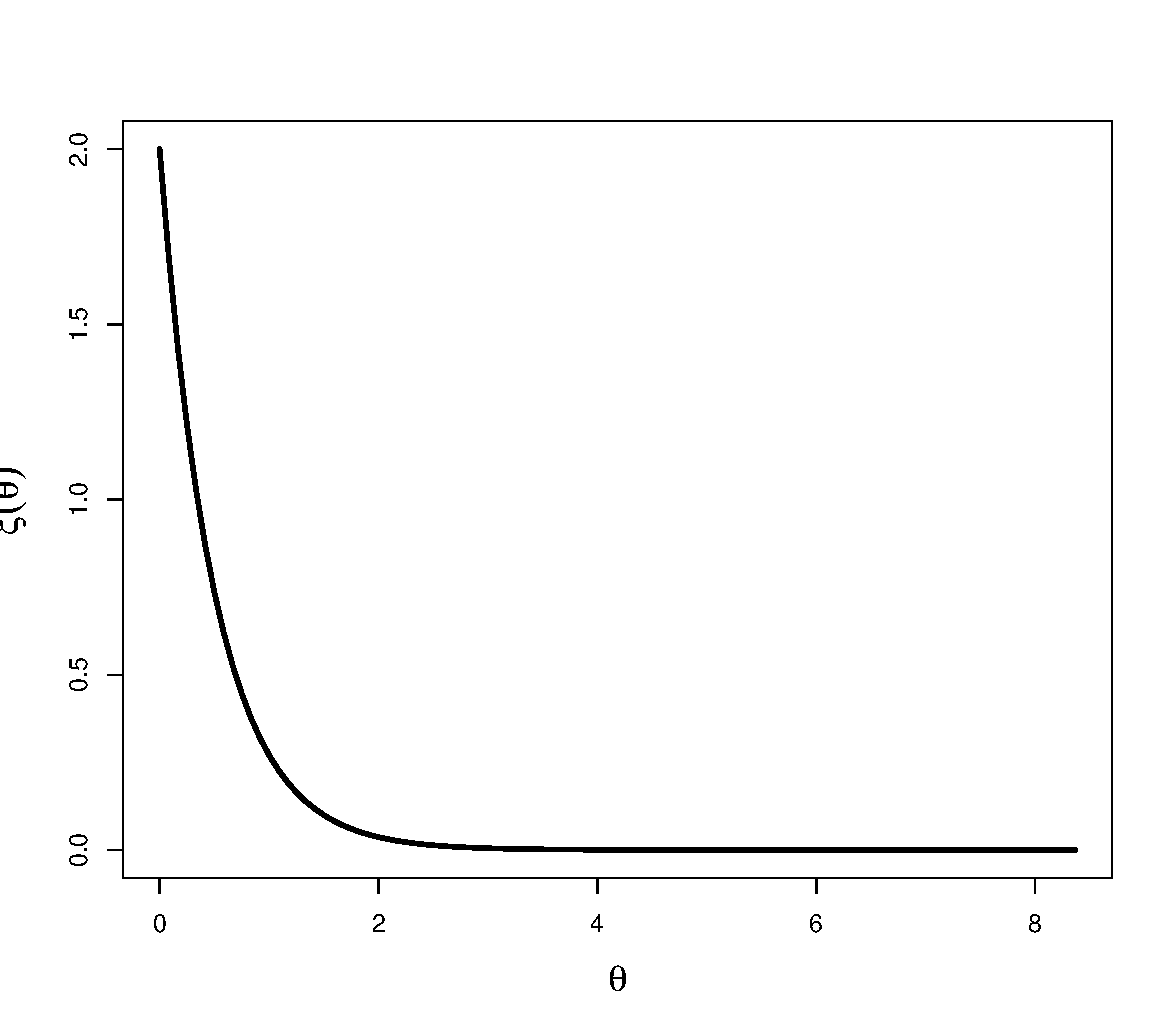
\includegraphics[scale=0.4]{figures/gamma_1_2.pdf} 
\end{center} 
\end{figure} 
\end{frame}
%%%%%%%%%%%%%%%%%%%%%%%%%%%%%%%%%%%
\begin{frame}{A distribuição~\textit{a priori}}
\begin{defn}
\label{def:prior}
 \textbf{Distribuição~\textit{a priori}}.
 Se tratamos o parâmetro $\theta$ como uma variável aleatória, então a distribuição~\textit{a priori}, que também chamaremos simplesmente de priori, é a distribuição que damos a $\theta$~\textbf{antes} de observarmos as outras variáveis aleatórias de interesse.
 Em geral, vamos denotar a função de densidade/massa de probabilidade da priori por $\xi(\theta)$.
\end{defn}
\textbf{Exemplos:}
\begin{itemize}
 \item Podemos dizer que a probabilidade de uma moeda cair cara, $p$, tem distribuição uniforme entre 0 e 1;
 \begin{itemize}
  \item Ou que tem distribuição $\operatorname{Beta}(2, 2)$;
 \end{itemize}
 \item A altura média dos jogadores de basquete do CR Flamengo tem distribuição normal com média $\mu_0 = 200 cm$ e variância $\sigma_0^2 = 25 cm^2$;
 \item A posição de Júpter em relação ao Sol hoje tem coordenadas $X,Y, Z$, de modo que $X \sim \operatorname{Normal}(\mu_x, 1)$, $Y \sim \operatorname{Normal}(\mu_y, 1)$, $Z \sim \operatorname{Normal}(\mu_z, 1)$.
\end{itemize}
\end{frame}
%%%%%%%%%%%%%%%%%%%%%%%%%%%%%%%%%%%
\begin{frame}{Distribuição~\textit{a posteriori}}
\begin{defn}
 \label{def:posterior}
 Considere o problema estatístico com parâmetro $\theta$ e variáveis aleatórias observáveis $\rs$.
 A distribuição condicional de $\theta$ dados os valores observados das variáveis aleatórias, $\boldsymbol x := \{x_1, x_2, \ldots, x_n \}$ é a~\textbf{distribuição~\textit{a posteriori}} de $\theta$.
 Denotamos por $\xi(\theta \mid \boldsymbol x)$ a f.d.p/f.m.p. condicional a $X_1 = x_1, X_2 = x_2, \ldots X_n = x_n$.
\end{defn}
\begin{theo}
 \label{thm:posterior_distribution}
 Considere a amostra aleatória $\rs$ de uma distribuição com f.d.p./f.m.p. $f(x\mid\theta)$.
 Se a distribuição~\textit{a priori} é $\xi(\theta)$, temos
 \begin{equation}
  \label{eq:posterior}
    \xi(\theta \mid \boldsymbol x) = \frac{\xi(\theta)\prod_{i=1}^n f(x_i \mid \theta)}{g_n(\boldsymbol x)}, \: \theta \in \Omega.  
 \end{equation}
 Chamamos $g_n(\boldsymbol x)$ de distribuição~\textit{marginal} de $\rs$.
\end{theo}
\textbf{Prova:} Usar a premissa de amostra aleatória para escrever $f(x_1, x_2, \ldots, x_n \mid \theta)$, escrever a distribuição conjunta de $\theta$ e $\boldsymbol x$ e computar $g_n(\boldsymbol x)$ usando a lei da probabilidade total. 
\end{frame}
%%%%%%%%%%%%%%%%%%%%%%%%%%%%%%%%%%%
\begin{frame}{Distribuição~\textit{a posteriori}: exemplo}
Continuando com o Exemplo~\ref{ex:duracao_componentes}, fica claro que 
 \[f (\boldsymbol x  \mid \theta) = \prod_{i=1}^n f(x_i \mid \theta) = \theta^n\exp(-S\theta), \]
onde $S = \sum_{i = 1}^n x_n$.
Desta forma, temos 
\[ f (\boldsymbol x  \mid \theta)\xi(\theta) = \theta^{n+1}\exp(-(S + 2)\theta).\]
Para obter $g_n(\boldsymbol{x})$, computamos 
\[ g_n(\boldsymbol{x}) = \int_0^\infty t^{n+1}\exp(-(S + 2)t) \,dt = \frac{\Gamma( n + 2) }{ (S + 2)^{n + 2}}. \]
Concluímos que 
\[\xi(\theta \mid \boldsymbol{x}) = \frac{(S + 2)^{n + 2}}{\Gamma( n + 2)} \theta^{n+1}\exp(-(S + 2)\theta),  \]
ou seja, $\theta \mid \boldsymbol{x} \sim \operatorname{Gama}(n + 2, \sum_{i = 1}^n x_n + 2)$.
\end{frame}
%%%%%%%%%%%%%%%%%%%%%%%%%%%%%%%%%%%
\begin{frame}{Distribuição~\textit{a posteriori}: exemplo (cont.)}
    \begin{figure}[!ht]
    \label{fig:posterior_componentes}
    \begin{center}
    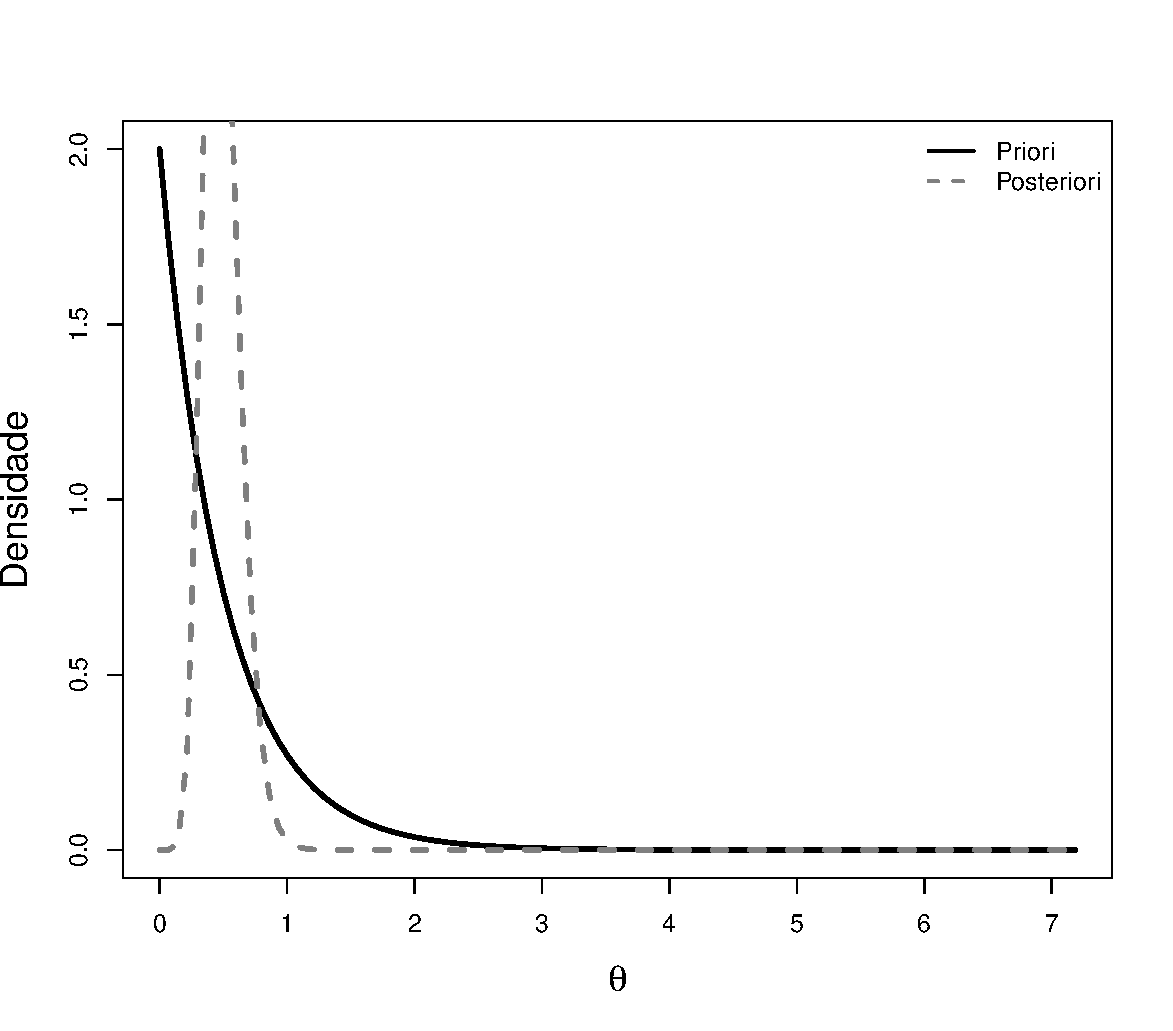
\includegraphics[scale=0.4]{figures/posterior_componentes.pdf} 
    \end{center} 
    \end{figure} 
\end{frame}
%%%%%%%%%%%%%%%%%%%%%%%%%%%%%%%%%%%
\begin{frame}{A função de verossimilhança}
 Note que o denominador em~(\ref{eq:posterior}) não depende do parâmetro, $\theta$.
 Deste modo, podemos escrever
 \[ \xi(\theta \mid \boldsymbol{x}) \propto f(\boldsymbol{x} \mid \theta)\xi(\theta), \]
 querendo dizer que os dois lados de $\propto$ são iguais a não ser talvez por uma constante que independe de $\theta$.
 Por vezes podemos escrever também $\xi(\theta \mid \boldsymbol{x}) \propto_\theta f(\boldsymbol{x} \mid \theta)\xi(\theta)$.
 \begin{defn}
  \textbf{Função de verossimilhança}. 
  Quando encaramos a f.d.p./f.m.p. $f(x_1, x_2, \ldots, x_n \mid \theta)$ como uma função do parâmetro $\theta$, chamamos esta função de~\textbf{função de verossimilhança}, e podemos denotá-la como $L(\theta ; \boldsymbol{x})$ ou, quando a notação não criar ambiguidade, simplesmente $L(\theta)$.
 \end{defn}
\end{frame}
%%%%%%%%%%%%%%%%%%%%%%%%%%%%%%%%%%%
\begin{frame}{Aprendizado bayesiano sequencial}
Ainda sobre o Exemplo~\ref{ex:duracao_componentes}, considere a primeira observação $x_1$ e a distribuição~\textit{a posteriori} baseada apenas nesta observação: $\xi_1(\theta \mid x_1) \propto f(x_1 \mid \theta)\xi(\theta)$.
Se assumirmos que $\rs$ são condicionalmente independentes dado $\theta$, podemos escrever 
\[\xi(\theta \mid x_1, x_2) \propto f(x_1, x_2 \mid \theta)\xi(\theta) = f(x_1 \mid \theta)f(x_2 \mid \theta)\xi(\theta) = f(x_2 \mid \theta)\xi_1(\theta \mid x_1). \]
    \begin{figure}[!ht]
    \label{fig:posterior_componentes_sequencial}
    \begin{center}
    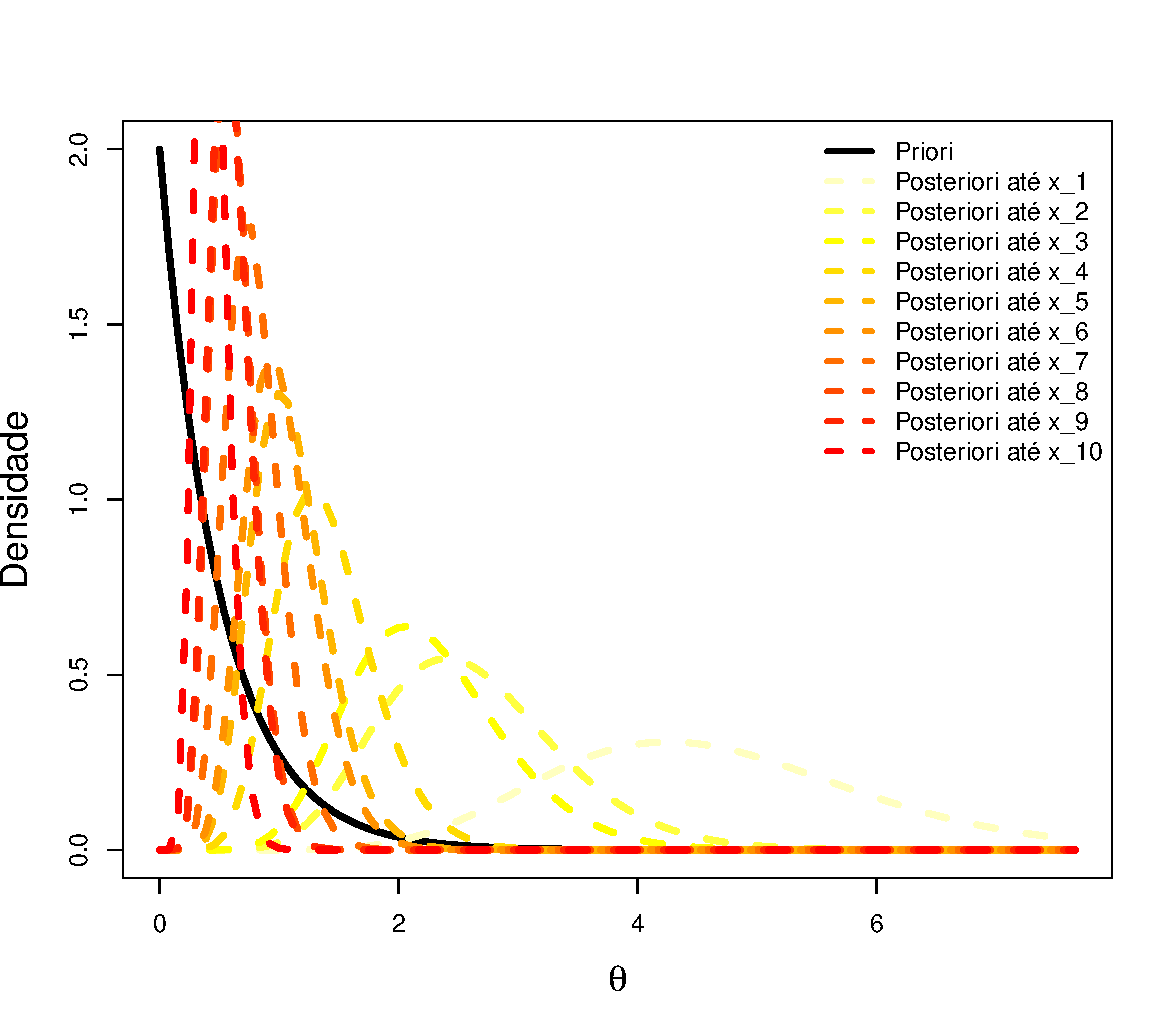
\includegraphics[scale=0.32]{figures/sequential_Bayes_componentes.pdf} 
    \end{center} 
    \end{figure} 
\end{frame}
%%%%%%%%%%%%%%%%%%%%%%%%%%%%%%%%%%%
\begin{frame}{Predição}
 Dentro do paradigma bayesiano, a predição de novos valores da(s) variável(is) aleatória(s) é feita a partir da distribuição~\textit{a posteriori},
 \begin{equation}
  \label{eq:posterior_prediction}
  p(x_{n+1} \mid x_1, x_2, \ldots, x_n) = \int_{\Omega} f(x_{n+1} \mid \theta)\xi(\theta \mid x_1, x_2, \ldots, x_n)\, d\theta.
 \end{equation}
Chamamos a distribuição condicional em~(\ref{eq:posterior_prediction}) de~\textbf{distribuição preditiva~\textit{a posteriori}}.
Em contraste, temos a~\textbf{distribuição preditiva~\textit{a priori}}:
 \begin{equation}
  \label{eq:prior_prediction}
  p(x_{n+1}) = \int_{\Omega} f(x_{n+1} \mid \theta)\xi(\theta)\, d\theta,
 \end{equation}
que é útil na aplicação de modelos bayesianos na prática, mas não será explorada aqui.
\end{frame}

%%%%%%%%%%%%%%%%%%%%%%%%%%%%%%%%%%%
\begin{frame}{O que aprendemos?}
\begin{itemize}
 \item[\faLightbulbO] Bayesianismo X frequentismo;
 
 ``Parâmetros como variáveis aleatórias ou constantes fixas e não-observáveis.''
 
 \item[\faHourglassStart] Distribuição~\textit{a priori}, $\xi(\theta)$;
 
 ``Nosso grau de crença~\underline{antes} de observamos dados.''
 
 \item[\faInfoCircle] Função de verossimilhança, $L(\theta) \propto f(\boldsymbol x \mid \theta)$;

 ``Codifica (toda) a informação sobre o modelo contida nos dados.''
 
 \item[\faHourglassEnd] Distribuição~\textit{a posteriori}, $\xi(\theta \mid \boldsymbol x) \propto L(\theta)\xi(\theta)$;
 
 ``Nossa crença atualizada a partir da informação contida em $L(\theta)$.''
 \end{itemize}
\end{frame}
%%%%%%%%%%%%%%%%%%%%%%%%%%%%%%%%%%%
\begin{frame}{Leitura recomendada}
\begin{itemize}
 \item[\faBook] De Groot seção 7.2;
 \item[\faBook] $^\ast$ Capítulo 1 de Schervish, M. J. (2012). Theory of statistics. Springer Science \& Business Media.
%  \item[‡\faGithub] .
\end{itemize} 
\end{frame}

\section*{Prioris conjugadas}
\begin{frame}{Prioris conjugadas}
 \begin{itemize}
  \item Prioris conjugadas
  \begin{itemize}
   \item Bernoulli;
   \item Poisson;
   \item Normal;
  \end{itemize}
\item Interpretação dos hiperparâmetros.
 \end{itemize}
\end{frame}

\begin{frame}{Caso conjugado: variáveis Bernoulli}
\begin{theo}[Posteriori Bernoulli]
\label{thm:Bernoulli_posterior}
 Sejam $\rs$ uma amostra aleatórias de variáveis aleatórias Bernoulli com parâmetro $p$, $ 0 < p < 1$, desconhecido.
 Suponha que a distribuição~\textit{a priori} de $p$ é uma distribuição Beta com parâmetros $\alpha > 0$ e $\beta > 0$.
 Seja $y = \sum_{i=1}^n X_i$. 
 Então
\[ \xi(p \mid \rs) = \frac{1}{B(\alpha + y, \beta + n -y)} p^{\alpha + y- 1} \left(1-p\right)^{\beta + (n-y) - 1}.\]
\end{theo}
\textbf{Prova:}
 Escrever a conjunta condicional como produto das marginais condicionais e notar que se obtêm o núcleo de uma distribuição Beta.
\end{frame}

\begin{frame}{Prioris conjugadas}

\begin{defn}[Hiperparâmetros]
\label{def:hyperparameters}
Seja $\xi(\theta \mid \phi)$ a distribuição~\textit{a priori} para o parâmetro $\theta$, indexada por $\phi \in \Phi$.
  Dizemos que $\phi$ é (são) o(s) \textbf{hiperparâmetro(s)} da priori de $\theta$.
 \end{defn}

\begin{defn}[\textbf{Priori conjugada}]
\label{def:conjugate_prior}
Suponha que $\irs$ sejam condicionalmente independentes dado $\theta$, com f.d.p./f.m.p. $f(x \mid \theta)$.
Defina
\[ \boldsymbol{\Psi} = \left\{ f : \Omega \to (0, \infty) ,  \int_{\Omega} f\, dx = 1  \right\}, \]
onde $\Omega$ é o espaço de parâmetros.
Dizemos que $\boldsymbol{\Psi}$ é uma~\textbf{família de distribuições conjugadas} para $f(x \mid \theta)$ se para toda $f \in \boldsymbol{\Psi}$ e toda realização $\boldsymbol{x}$ de $\boldsymbol X = \boldsymbol{\rs}$,
\[ \frac{f(\boldsymbol{x} \mid \theta) f(\theta)}{\int_{\Omega} f(\boldsymbol{x} \mid \theta) f(\theta)\,d\theta} \in \boldsymbol{\Psi}. \]
\end{defn}
Isto é, uma família de prioris é conjugada para uma determinada verossimilhança se a posteriori está na mesma família.
\end{frame}

\begin{frame}{Variância de uma posteriori Beta e critérios de parada}
 Se $X \sim \operatorname{Beta}(a, b)$, $\vr(X) = \frac{ab}{(a+b)^2(a + b+ 1)}$.
 Na situação do Teorema~\ref{thm:Bernoulli_posterior}, temos
 \begin{equation}
  \label{eq:beta_posterior_variance}
 V_n := \vr(p \mid \boldsymbol{x}) = \frac{(\alpha + y)(\beta + n - y)}{(\alpha + \beta + n)^2(\alpha + \beta + n + 1)}.  
 \end{equation}
 Podemos usar a expressão em~(\ref{eq:beta_posterior_variance}) para desenhar um experimento.
 Por exemplo, podemos coletar dados até que $V_n \leq 0.01$ (ver exercício 2, seção 7.3 de DeGroot). 
\end{frame}

\begin{frame}{Poisson e prioris Gamma}
 \begin{theo}[Posteriori para taxa da Poisson]
 \label{thm:Poisson_conjugate_inference}
  Suponha que $\rs$ formam uma amostra aleatória com distribuição Poisson com taxa $\theta > 0$, desconhecida.
  Suponha que a distribuição~\textit{a priori} para $\theta$ é uma distribuição Gama com parâmetros $\alpha >0$ e $\beta > 0$.
  Então
  \begin{equation}
   \xi(\theta \mid \boldsymbol{x}) = \frac{ (\beta + n)^{\alpha + S} }{\Gamma(\alpha + S)} \theta^{\alpha+S-1} e^{-(\beta+n)\theta},
  \end{equation}
  onde $S = \sum_{i=1}^n x_i$.
 \end{theo}
\textbf{Prova:} Análoga ao exemplo Bernoulli.
\end{frame}

\begin{frame}{Análise conjugada da normal com variância conhecida}
 \begin{theo}[Distribuição~\textit{a posteriori} da média de uma normal]
 \label{thm:posterior_normal_mean}
  Suponha que $\rs$ formam uma amostra aleatória com distribuição normal com média desconhecida $\theta$ e variância $\sigma^2 >0$, conhecida e fixa.
  Suponha que $\theta \sim \operatorname{Normal}(\mu_0, v_0^2)$~\textit{a priori}.
  Então
  \begin{equation}
   \xi(\theta \mid \boldsymbol{x}, \sigma^2) =  \frac{1}{\sqrt{2\pi\sigma^2}} \exp\left( \frac{(\theta-\mu_1)^2}{2v_1^2} \right),
  \end{equation}
onde
\begin{equation}
\mu_1 := \frac{\sigma^2 \mu_0 + nv_0^2\bar{x}_n}{\sigma^2 + nv_0^2} \quad\text{e}\quad v_1^2 := \frac{\sigma^2v_0^2}{\sigma^2 + nv_0^2}
\end{equation}
\end{theo}
\textbf{Prova:} Escrever as densidades relevantes sem as constantes de proporcionalidade, completar o quadrado (duas vezes) e notar que se obtem o núcleo de uma normal (Gaussiana).
\end{frame}

\begin{frame}{Interpretando a média~\textit{a posteriori}}
 Podemos reescrever $\mu_1$ como
 \begin{equation}
 \label{eq:posterior_mean_normal}
  \mu_1 = \frac{\sigma^2}{\sigma^2 + nv_0^2}\mu_0 + \frac{nv_0^2}{\sigma^2 + nv_0^2}\bar{x}_n.
 \end{equation}
\begin{obs}[Média~\textit{a posteriori} como média ponderada]
 No caso normal, a média~\textit{a posteriori} pode ser vista como uma~\textbf{média ponderada} entre a média~\textit{a priori} e a média amostral, sendo os pesos dados pela variância (conhecida) da distribuição dos dados e a variância da priori, $v_0^2$.
\end{obs}
\end{frame}

\begin{frame}{O que aprendemos?}
 \begin{itemize}
  \item[\faLightbulbO] Prioris conjugadas;
  \item[\faLightbulbO] Análise conjugada de
  \begin{itemize}
   \item Bernoulli;
   \item Poisson;
   \item Normal.
  \end{itemize}
 \end{itemize}
\end{frame}

\begin{frame}{Leitura recomendada}
\begin{itemize}
 \item[\faBook] DeGroot seção 7.3;
 \item[\faForward] Próxima aula: DeGroot, seção 7.4;
 \item {\large\textbf{Exercícios recomendados}}
 \begin{itemize}
  \item[\faBookmark] DeGroot, seção 7.3: exercícios 2, 17, 19, 21. 
  \end{itemize}
 \end{itemize} 
\end{frame}

\section*{Estimadores de Bayes}
\begin{frame}{Estimadores de Bayes}
 \begin{itemize}
  \item  Estimador e estimativa;
  \item Função de perda;
  \item Estimador de Bayes;
  \item Consistência do estimador de Bayes;
  \item Estimador de Bayes para grandes amostras;
  \item Limitações.
 \end{itemize}
\end{frame}


\begin{frame}{Prioris impróprias}
 \begin{defn}[Priori imprópria]
 Seja $\xi : \Lambda \to (0, \infty)$, $\Omega \subseteq \Lambda$, uma função tal que $\int_{\Omega} \xi(\theta)\,d\theta = \infty$.
 Se utilizamos $\xi$ como uma p.d.f. para $\theta$, dizemos que $\xi$ é uma~\textbf{priori imprópria} para $\theta$.
 \end{defn}
\begin{exemplo}[Priori imprópria para a taxa de uma Poisson]
   Suponha que $\rs$ formam uma amostra aleatória com distribuição Poisson com taxa $\theta > 0$, desconhecida.
   Desta vez, fazemos a escolha de hiperparâmetros $\alpha = \beta = 0$, o que leva a 
   \begin{equation*}
    \xi(\theta) = \frac{1}{\theta}.
   \end{equation*}
A posteriori passa a ser 
  \begin{equation*}
   \xi(\theta \mid \boldsymbol{x}) = \frac{ n^{S} }{\Gamma(S)} \theta^{n-1} e^{-S\theta},
  \end{equation*}
   onde $S = \sum_{i=1}^n x_i$.
\end{exemplo}
\end{frame}

\begin{frame}{Estimadores (de Bayes)}

\begin{defn}[Estimador]
Sejam $\rs$ variáveis aleatórias com distribuição conjunta indexada por $\theta$.
Um~\textbf{estimador} de $\theta$ é qualquer função real $\delta: \rs \to \mathbb{R}^d$, $d\geq 1$. 
\end{defn}
\begin{defn}[Estimativa]
Dizemos que o valor de $\delta$ avaliado nas realizações de $\rs$, $\boldsymbol x = \{ x_1, x_2, \ldots, x_n\}$,  $\delta(\boldsymbol{x})$ é uma~\textbf{estimativa} de $\theta$.
\end{defn}

\begin{defn}[Função de perda]
Uma função de perda é uma função real em duas variáveis 
\[ L : \Omega \times \mathbb{R}^d \to \mathbb{R}, \]
em que dizemos que o estatístico~\underline{perde} $L(\theta, a)$ se o parâmetro vale $\theta$ e a estimativa dada vale $a$.
\end{defn} 
\end{frame}

\begin{frame}{Funções de perda e estimadores bayesianos}
Exemplos de funções de perda são $L(\theta, a) = (\theta-a)^2$ e $L(\theta, a) = |\theta-a|$.
\begin{obs}[Perda esperada~\textit{a priori}]
Se escolhemos uma priori $\xi(\theta)$, nossa perda esperada,~\textbf{antes} de observar os dados é
\begin{equation*}
 E_\xi[L(\theta, a)] = \int_{\Omega} L(\theta, a)\xi(\theta)\,d\theta.
\end{equation*}
Vemos então que a escolha da distribuição~\textit{a priori} está inextrincavelmente ligada à função de perda.
\end{obs}
\end{frame}

\begin{frame}{Estimador de Bayes}
 \begin{defn}[Estimador de Bayes]
  Considere a perda esperada~\textit{a posteriori}:
  \begin{equation*}
   E_{\theta \mid \boldsymbol{x}}\left[L(\theta, a) \right] = E[L(\theta, a) \mid \boldsymbol{x}] = \int_{\Omega} L(\theta, a)\xi(\theta \mid \boldsymbol{x})\, d\theta. 
  \end{equation*}
Dizemos que $\delta^\ast$ é um~\textbf{estimador de Bayes} se, para toda realização $\boldsymbol{X} = \boldsymbol{x}$,
\begin{equation*}
 E[L(\theta, \delta^\ast(\boldsymbol{x}) ) \mid \boldsymbol{x}] = \min_{a \in \mathcal{A}}   E[L(\theta, a) \mid \boldsymbol{x}].
\end{equation*}
 \end{defn}
\begin{itemize}
 \item Em outras palavras, um estimador de Bayes é uma função real dos dados que minimiza a perda esperada com respeito à posteriori dos parâmetros.
\end{itemize} 
\end{frame}

\begin{frame}{Estimador de Bayes sob perda quadrática}
Suponha que a função de perda seja 
\[ L(\theta, \delta^\ast) =  (\theta-\delta^\ast)^2. \]
Dizemos que a função de perda é~\textbf{quadrática}.
Temos o seguinte resultado:
 \begin{theo}[$\delta^\ast$ sob perda quadrática]
  \label{thm:posterior_mean_quadratic}
  (De Groot, Corolário 7.4.1)
  
  Seja $\theta$ um parâmetro tomando valores reais.
  Sob perda quadrática,
  $$\delta^\ast(\boldsymbol{x}) = E[\theta | \boldsymbol{X} = \boldsymbol{x}] = \int_{\Omega} \theta \xi(\theta \mid \boldsymbol{x} ) \,d\theta.$$
 \end{theo}
 \textbf{Prova:} Escrever a perda esperada~\textit{a posteriori} explicitamente, usar a lei de esperanças e minimizar a expressão resultante com respeito ao estimador (ex. diferenciar e igualar a derivada a zero).
\end{frame}

\begin{frame}{Estimador de Bayes sob perda absoluta}
 \begin{theo}[$\delta^\ast$ sob perda absoluta]
  \label{thm:posterior_median_absolute}
  (De Groot, Corolário 7.4.2)
  
  Suponha que a função de perda é dada por  
\[ L(\theta, \delta^\ast) =  |\theta-\delta^\ast|. \]
Dizemos que a função de perda é~\textbf{absoluta}.
  
  Seja $\theta$ um parâmetro tomando valores na reta.
  Sob perda absoluta, $\delta^\ast(\boldsymbol{x})$ é a~\textbf{mediana}~\textit{a posteriori}, isto é,
  $$\int_{-\infty}^{\delta^\ast(\boldsymbol{x})}\xi(\theta \mid \boldsymbol{x} ) \,d\theta = \frac{1}{2}.$$
 \end{theo}
 \textbf{Prova:} Decompor a perda esperada em duas integrais de funções não-negativas utilizando as propriedades da função valor absoluto e aplicar a regra de Leibnitz duas vezes para encontrar o ponto de mínimo.
\end{frame}


\begin{frame}{O estimador de Bayes em grandes amostras}
\begin{itemize}
 \item Sob condições brandas de regularidade, à medida que o tamanho de amostra cresce, a influência da priori diminui.
\end{itemize}

\begin{exemplo}[Proporção de itens defeituosos]
Suponha que estamos interessados na proporção $\theta$ de itens defeituosos em uma linha de produção.
Suponha ainda que
\begin{itemize}
 \item Priori 1: $\xi_1(\theta) = 1$, $0 < \theta < 1$;
 \item Priori 2: $\xi_2(\theta) = 2(1-\theta)$, $0 < \theta < 1$;
 \item Dados: de $n = 100$ itens observados, $y = 10$ apresentaram defeito.
\end{itemize}

Perguntas:
\begin{itemize}
 \item $\bar{x}_n$ = ?
 \item $E_1[\theta \mid \boldsymbol{x}] = \int_{0}^1 \theta \xi_1(\theta \mid \boldsymbol{x})\,d\theta$ = ?
%  \item $E_2[\theta \mid \boldsymbol{x}] = \int_{0}^1 \theta \xi_2(\theta \mid \boldsymbol{x})\,d\theta$ = ?
\end{itemize} 
\end{exemplo}
\end{frame}

\begin{frame}{Proporção de itens defeituosos: prioris e posterioris}
Ver também exemplo 7.3.3 de De Groot.
\begin{figure}[!ht]
\label{fig:defect_items}
\begin{center}
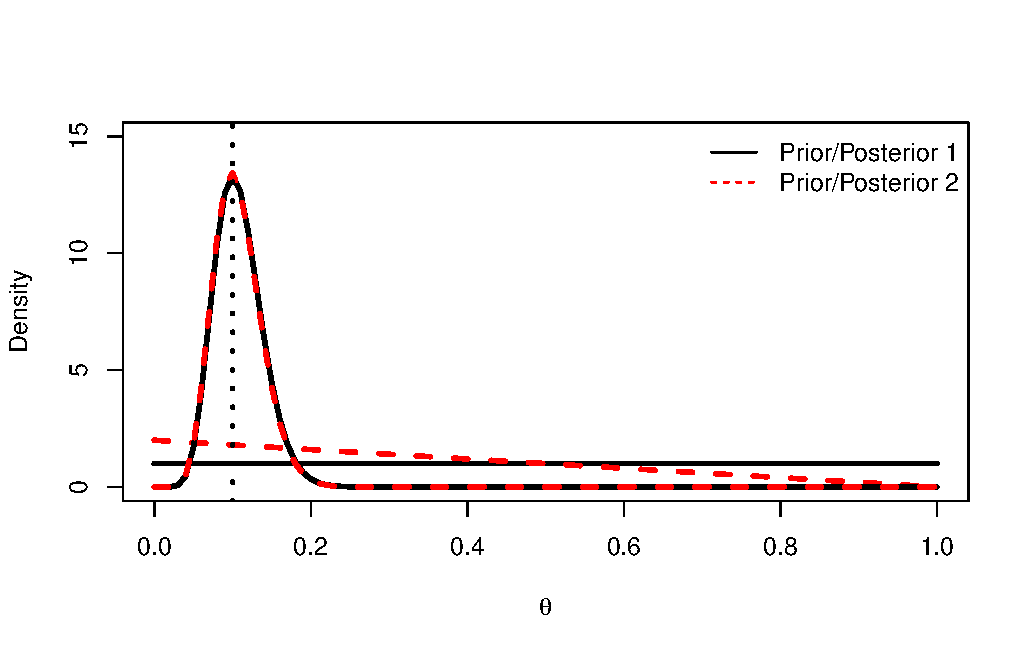
\includegraphics[scale=0.65]{figures/defeituosos.pdf} 
\end{center} 
\end{figure} 
\end{frame}


\begin{frame}{Consistência do estimador de Bayes}
\begin{defn}[Estimador consistente]
Seja $\delta_1, \delta_2, \ldots, \delta_n$ uma sequência de estimadores de $\theta$.
Se quando $n \to \infty$ a sequência converge para $\theta$, dizemos que esta é uma sequência consistente de estimadores.
\end{defn} 

\begin{obs}[A média amostral é consistente para o caso Bernoulli]
 Se $\rs$ são i.i.d. Bernoulli com parâmetro $\theta$ condicional a $\theta$, temos pela LGN: $\bar{X}_n \xrightarrow{\text{p}} \theta$.
\end{obs}

\begin{obs}[O estimador de Bayes é consistente para o caso Bernoulli]
 Para $\alpha > 0$ e $\beta > 0$ fixos, a média~\textit{a posteriori} vale
 $$\delta^\ast(\boldsymbol{x}) = E[\theta \mid \boldsymbol{x}] = \frac{\alpha + y}{\alpha + \beta + n}, $$
 onde $ y = \sum_{i=1}^n x_i$.
 É fácil ver que $\delta^\ast(\boldsymbol{x}) \xrightarrow{\text{p}} \bar{x}_n \xrightarrow{\text{p}} \theta$.
\end{obs}


\end{frame}

\begin{frame}{O que aprendemos?}
\begin{itemize}
 \item[\faLightbulbO] Estimador;
 
  ``Um estimador é qualquer função real dos dados''
  
 \item[\faLightbulbO] Função de perda;
 
  ``Uma função real que quantifica a perda incorrida por uma estimativa incorreta'' 
 
 \item[\faLightbulbO] Estimador de Bayes;
 
  ``Um estimador que minimiza a perda esperada~\textit{a posteriori}''
  
 \item[\faLightbulbO] Propriedades e limitações do estimador de Bayes;
 
  ``À medida que o tamanho da amostra cresce, o estimador se aproxima do valor verdadeiro, a influência da priori diminui, mas precisamos sempre de uma função de perda bem especificada'' 
 \end{itemize}
 
 \end{frame}

\begin{frame}{Leitura recomendada}
\begin{itemize}
 \item[\faBook] De Groot seção 7.4;
 \item[\faBook] $^\ast$ Casella \& Berger, seção 7.2.3.
 \item {\large\textbf{Exercícios recomendados}}
 \begin{itemize}
  \item[\faBookmark] De Groot, seção 7.4: exercícios 2, 4, 7, 11 e 14.
  \end{itemize}
 \end{itemize} 
\end{frame}



\section*{Estimador de máxima verossimilhança (EMV)}
\begin{frame}{Tópicos da aula}
 \begin{itemize}
  \item Estimador de máxima verossimilhança (EMV);
  \begin{itemize}
     \item Existência e unicidade;
     \item Invariância do EMV;
     \item Consistência do EMV;
  \end{itemize}
  \item Limitações;
 \end{itemize}
\end{frame}

\begin{frame}{Estimador de máxima verossimilhança (EMV)}
 \begin{defn}[Estimador de máxima verossimilhança]
 \label{def:MLE}
  Para cada possível vetor (de observações) $\boldsymbol{x}$, seja $\delta(\boldsymbol{x}) \in \Omega$ um valor de $\theta \in \Omega$ de modo que a função de verossimilhança, $L(\theta) \propto f(\boldsymbol{x} \mid \theta)$, atinge o máximo.
  Dizemos que $\hat{\theta} = \delta(\boldsymbol{X})$ é o~\textbf{estimador de máxima verossimilhança} de $\theta$ (Fisher, 1922)\footnote{Ronald Aylmer Fisher (1890-1962), biólogo e estatístico inglês. Para a história do desenvolvimento do EMV, ver~\href{https://projecteuclid.org/euclid.ss/1030037906}{Aldrich (1997)}.}.
  Quando observamos $\boldsymbol{X} = \boldsymbol{x}$, dizemos que $\delta(\boldsymbol{x})$ é uma~\textit{estimativa} de $\theta$.
  Dito de outra forma,
   $$ \max_{\theta \in \Omega} f(X \mid \theta) = f(X\mid \hat{\theta}).$$
 \end{defn}
\end{frame}

\begin{frame}{Mudando de paradigma}
Na Definição~\ref{def:MLE}, vemos $\theta$ com um número real que indexa a distribuição de probabilidade conjunta dos dados.

\begin{itemize}
 \item Poderíamos trocar\footnote{Mas não vamos, pois a notação fica clara em quase todos os contextos.} $f(x \mid \theta)$ por $f(x; \theta)$;
 \item Com o EMV, procuramos um valor de $\theta$ de modo que a probabilidade de observarmos $\boldsymbol{X} = \boldsymbol{x}$ seja máxima;
 \item Isso não nos diz nada sobre o quão provável $\hat{\theta}$ é;
 \item $\theta$ não é uma quantidade aleatória, portanto não admite afirmações probabilísticas.
\end{itemize}
\end{frame}

\begin{frame}{Exemplos}
 \begin{itemize}
  \item Exponencial;
  \item Bernoulli;
  \item Normal;
  \begin{itemize}
   \item $\mu$ desconhecida, $\sigma^2$ conhecida;
   \item $\mu$ conhecida, $\sigma^2$ desconhecida;
   \item $\mu$ e $\sigma^2$ ambas desconhecidas.
  \end{itemize}
 \end{itemize}
\end{frame}

\begin{frame}{EMVs}
 \begin{itemize}
  \item Exponencial: $\hat{\theta} = 1/\bar{X}_n$;
  \item Bernoulli $\hat{\theta} = \bar{X}_n$;
  \item Normal;
  \begin{itemize}
   \item $\hat{\mu} = \bar{X}_n$;
   \item $\hat{\sigma^2} = \frac{1}{n}\sum_{i=1}^n (X_i - \mu)^2$;
   \item $\hat{\theta} = \left\{ \hat{\mu} = \bar{X}_n,  \hat{\sigma^2} = \frac{1}{n}\sum_{i=1}^n (X_i - \bar{X}_n)^2 \right\}$.
  \end{itemize}
 \end{itemize}
\end{frame}

\begin{frame}{EMV para uma distribuição uniforme}

\begin{exemplo}[EMV para uniforme]
\label{ex:uniform_closed}
 Suponha que $\rs$ perfazem uma amostra aleatória de uma distribuição uniforme no intervalo $[0, \theta]$, $\theta \in \mathbb{R}, \theta > 0$.
 Considere a f.d.p.
 \begin{equation}
  \label{eq:uniform_closed}
  f(x\mid \theta)=
 \begin{cases}
     \frac{1}{\theta}, 0 \leq x \leq \theta,\\
     0,\:\text{caso contrário}.
\end{cases}
  \end{equation}
A f.d.p. conjunta é
\begin{equation}
 \label{eq:uniform_closed_joint}
   f_n(\boldsymbol{x} \mid \theta)=
 \begin{cases}
     \theta^{-n}, 0 \leq x_i \leq \theta \: (i = 1, 2, \ldots, n),\\
     0,\:\text{caso contrário},
\end{cases}
\end{equation}
e o EMV é $\hat{\theta} = \max(x_1, x_2, \ldots, x_n)$.
\end{exemplo}
\end{frame}

\subsection*{Existência} 
\begin{frame}{Existência do EMV}
\begin{obs}
A existência do EMV pode depender de detalhes irrelevantes acerca do espaço de parâmetros, $\Omega$. 
\end{obs}
\begin{exemplo}[Não existência do EMV]
 Considere o Exemplo~\ref{ex:uniform_closed}, mas agora com uma f.d.p. um pouco diferente:
 \begin{equation}
  \label{eq:uniform_open}
    f(x\mid \theta)=
 \begin{cases}
     \frac{1}{\theta}, 0 < x < \theta,\\
     0,\:\text{caso contrário}.
\end{cases}
 \end{equation} 
É fácil mostrar que, nesse caso, o EMV não existe. 
\end{exemplo}
\end{frame}

\subsection*{Unicidade} 

\begin{frame}{Unicidade do EMV}

\begin{obs}[Unicidade do EMV]
Mesmo quando existe, o EMV nem sempre é único. 
\end{obs}

\begin{exemplo}[EMV para uma uniforme num intervalo de tamanho $1$]
 Suponha que $\rs$ perfazem amostra aleatória de uma distribuição uniforme no intervalo $[\theta, \theta + 1]$.
A densidade conjunta é
  \begin{equation}
  \label{eq:uniform_thetapOne}
    f_n(\boldsymbol{x}\mid \theta)=
 \begin{cases}
     1, \theta \leq x_i \leq \theta + 1, \: (i = 1, 2, \ldots, n),\\
     0,\:\text{caso contrário}.
\end{cases}
 \end{equation}
Defina $m := \min(x_1, x_2, \ldots, x_n)$ e $M := \max(x_1, x_2, \ldots, x_n)$.
Podemos reescrever~(\ref{eq:uniform_thetapOne}) como 
  \begin{equation}
  \label{eq:uniform_thetapOne_b}
    f_n(\boldsymbol{x}\mid \theta)=
 \begin{cases}
     1, M - 1 \leq \theta \leq m, \: (i = 1, 2, \ldots, n),\\
     0,\:\text{caso contrário}.
\end{cases}
 \end{equation}
\end{exemplo}
\textbf{Conclusão:} $\hat{\theta}$ é qualquer valor no intervalo $[M-1, m]$.
\end{frame}
 
\subsection*{Invariância} 

\begin{frame}{Invariância do EMV}
Suponha que estamos interessados em uma transformação do parâmetro $\theta$, $\phi(\theta)$.
Por exemplo, se $\rs$ são Bernoulli com parâmetro $p$,  podemos estar interessados na~\textit{chance} $\omega = \phi(p) = p/(1-p)$.
\begin{theo}[Invariância do EMV]
 Considere uma função $\phi : \Omega \to \mathbb{R}$.
 Se $\hat{\theta}$ é um EMV para $\theta$, então $\phi(\hat{\theta})$ é um EMV para $\omega = \phi(\theta)$.
\end{theo}
\textbf{Prova:} Defina a~\textit{verossimilhança induzida}:
\[ L^\ast(\omega) := \sup_{\left\{ \theta: \phi(\theta) = \omega \right\}} L(\theta), \]
e note que o supremo desta função sobre $\Omega$ é precisamente o EMV.
Ver Casella \& Berger, Teorema 7.2.10 (pág. 320) ou De Groot, Teorema 7.6.2 (pág 427).
\textbf{Exemplo:} O EMV para o quadrado da média de uma normal, $\mu^2$, é $\bar{X}_n^2$.
\end{frame}

\subsection*{Consistência} 

\begin{frame}{Consistência do EMV}
Sob condições de regularidade, o EMV é consistente, isto é $\hat{\theta}_{\text{EMV}} \xrightarrow{} \theta$.
\begin{theo}[Consistência do EMV]
Defina $l(\theta) := \log f_n(\boldsymbol{x} \mid \theta)$ e assuma que $\rs \sim f(\theta_0)$, isto é, que $\theta_0$ é o valor verdadeiro do parâmetro.
Denote $E_{\theta_0}[g] := \int_{\Omega} g(x, \theta) f(\boldsymbol{x} \mid \theta_0)\, dx$.
 Suponha que 
 \begin{itemize}
  \item $f(x_i \mid \theta)$ tem o mesmo suporte;
  \item $\theta_0$ é ponto interior de $\Omega$;
  \item $l(\theta)$ é diferenciável;
  \item $\hat{\theta}_{\text{EMV}}$ é a única solução de $l^\prime(\theta) = 0$.
 \end{itemize}
   Então,
  $$\hat{\theta}_{\text{EMV}} \xrightarrow{} \theta.$$
\end{theo}
\textbf{Prova:} (rascunho) mostrar que, para todo $\theta \in \Omega$,
\[ \frac{1}{n} \sum_{i=1}^n \log f(X_i \mid \theta) \xrightarrow{} E_{\theta_0}\left[ \log f(\boldsymbol{X} \mid \theta) \right], \]
e aplicar a desigualdade de Jensen.
\end{frame}

\begin{frame}{O que aprendemos?}
\begin{itemize}
 \item[\faLightbulbO] Estimador de máxima verossimilhança (EMV);
 
   ``Encontrar o valor do parâmetro que maxima a probabilidade observar os dados obtidos''
   
  \item[\faLightbulbO] Invariância ;
  
  ``O EMV é invariante a transformações dos parâmetros; se $\hat{\theta}$ é o EMV para $\theta$, $\psi(\hat{\theta})$ é o EMV para $\psi(\theta)$''
  
    \item[\faLightbulbO] Consistência;
  
  ``Sob condições brandas de regularidade, o EMV converge para valor verdadeiro à medida que $n \to \infty$''
  
    \item[\faLightbulbO] Limitações;
  
  ``O EMV não existe necessariamente, e, mesmo quando existe, não precisa ser único''
  
  \end{itemize}
 \end{frame}

\begin{frame}{Leitura recomendada}
\begin{itemize}
 \item[\faBook] De Groot seções 7.5 e 7.6;
 \item[\faBook] $^\ast$ Casella \& Berger, seção 7.2.2.
 \item[\faBook] $^\ast$ Schervish (1995), seção 5.1.3.
 \item {\large\textbf{Exercícios recomendados}}
 \begin{itemize}
  \item[\faBookmark] De Groot,
  \begin{itemize}
   \item Seção 7.5: exercícios  1, 4, 9 e 10;
   \item Seção 7.6: exercícios 3, 5 e 11.
  \end{itemize}   
  \end{itemize}
 \end{itemize} 
\end{frame}


\begin{frame}{Comparando métodos de estimação}
 \begin{itemize}
  \item Estimadores de Bayes~\textit{vs} EMV;
  \item Método dos momentos
 \end{itemize}
\end{frame}

\begin{frame}{Bayes~\textit{vs} EMV}
Argumentos asintóticos:
  \begin{equation*}
   L(\theta) \approx \exp\left[-\frac{\left(\theta-\hat{\theta}\right)^2}{2V_n(\theta)/n} \right].
  \end{equation*}
 \begin{exemplo}[ Exemplo 7.6.11 em De Groot]
    $\rs \sim \operatorname{Exponencial}(\theta)$, 
    \begin{itemize}
     \item   $\hat{\theta}_{\text{EMV}} = \left(\bar{X}_n\right)^{-1} \implies E[\hat{\theta}_{\text{EMV}}] = \theta$ e $\vr[\hat{\theta}_{\text{EMV}}] = \theta^2$.
  Pelo método Delta, temos $\hat{\theta}_{\text{EMV}} \approx \operatorname{Normal}(\theta, \theta^2/n)$;
    \item Se escolhemos uma priori gama para $\theta$ com hiperparâmetros $\alpha > 0$ e $\beta > 0$,    temos $E_{\theta \mid \boldsymbol{x}}[\theta] = (\alpha + n)/(\beta + S_n)$ e $\vr_{\theta \mid \boldsymbol{x}}(\theta) = (\alpha + n)/ (\beta + S_n)^2$.
    Fazendo $\alpha, \beta \ll n$, temos um argumento análogo para o estimador de Bayes.
    \end{itemize}  
 \end{exemplo}
\end{frame}


\begin{frame}{EMV para taxa de uma exponencial (DG ex. 7.6.11)}
\begin{figure}[!ht]
\label{fig:mle_exponential_deltaMethod}
\begin{center}
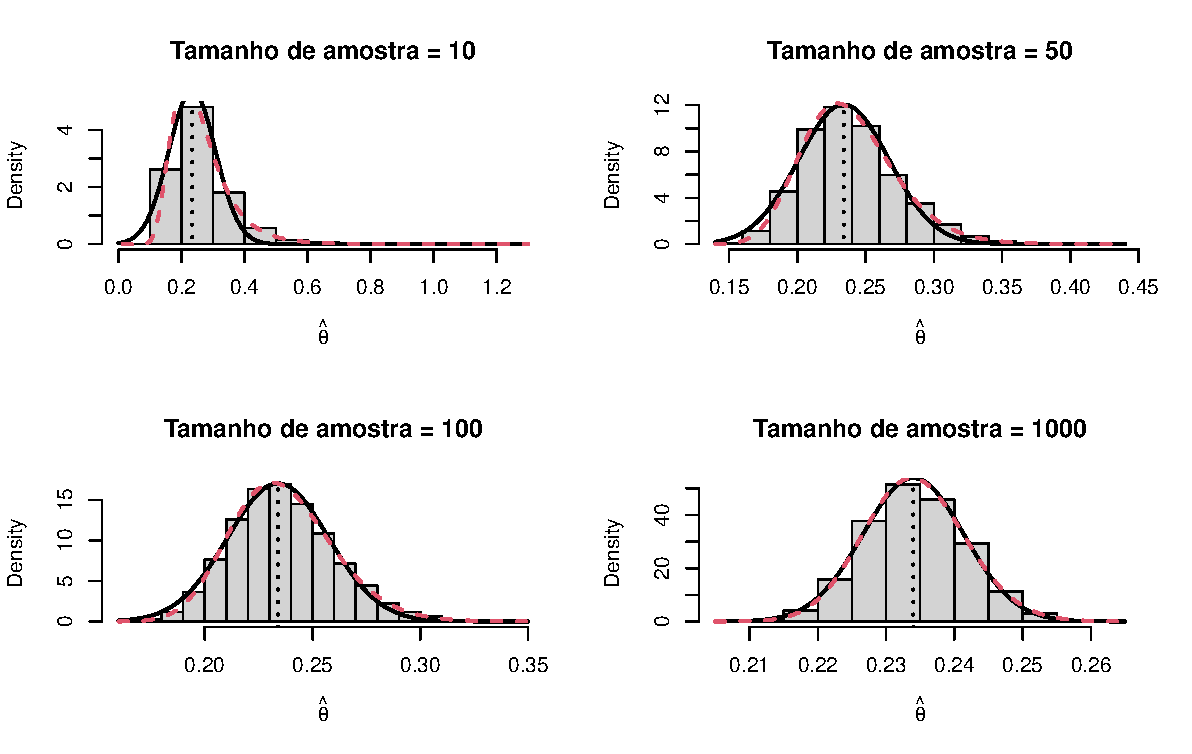
\includegraphics[scale=0.6]{figures/exponential_mle_deltaMethod.pdf} 
\end{center} 
\end{figure} 
\end{frame}

\begin{frame}{Inferência para uma Uniforme em $(0, \theta)$}
\begin{exemplo}[Exemplo 7.6.14 em De Groot]
$\rs \sim \operatorname{Uniforme}(0, \theta)$.
Definindo $Y = \max(\rs)$ temos 
\[ g_n(y \mid \theta) = n\frac{y^{n-1}}{\theta^n}. \]
Como já discutido, temos $\hat{\theta}_{\text{EMV}} = \max(\rsd) = y_n$ e portanto
\begin{itemize}
 \item $E[\hat{\theta}_{\text{EMV}}] = \frac{n}{n + 1}\theta$;
 \item $\vr(\hat{\theta}_{\text{EMV}}) =  \frac{n}{(n + 1)^2(n+2)}\theta^2$.
\end{itemize}
Do lado bayesiano, vamos obter a posteriori (com uma priori imprópria):
  \begin{equation}
  \label{eq:uniform_reference_posterior}
    \xi(\theta \mid \boldsymbol{x})=
 \begin{cases}
     \frac{(n-1)y_n^{n-1}}{\theta^n}, y_n < \theta,\\
     0,\:\text{caso contrário}.
\end{cases}
 \end{equation}
Isto nos leva a
\begin{itemize}
 \item $E[\hat{\theta}_{\text{Bayes}}] = \frac{n-1}{n-2}y_n$;
 \item $\vr(\hat{\theta}_{\text{Bayes}}) =  \frac{n-1}{(n - 2)^2(n-3)}y_n^2$.
\end{itemize}
\end{exemplo}
\end{frame}

\begin{frame}{Método dos momentos (MM)}
 Algumas vezes, obter o EMV ou o estimador de Bayes envolve dificuldades numéricas (ex. estimar os parâmetros de uma distribuição Gama).
 Nestas situações, podemos encontrar um estimador para os parâmetros que relacione os momentos empíricos com os téoricos.
 
 \begin{defn}[Método dos momentos]
  Suponha que $\rs$ formam uma amostra aleatória com distribuição conjunta $f_n(\rs \mid \theta)$, $\theta \in \Omega \subseteq \mathbb{R}^k$ e que o $k$-ésimo momento existe.
  Defina $\mu_j(\theta) = E[X_1^j \mid \theta]$ e suponha que $\mu : \Omega \to  \mathbb{R}^k$ é biúnivoca, de modo que sua inversa é 
  \[ \theta = M(\mu_1(\theta), \ldots, \mu_k(\theta)).\]
 Dados os~\textit{momentos amostrais} $m_j := \frac{1}{n} \sum_{i=1}^n X_i^j$, $j = 1, \ldots, k$, o~\textbf{estimador de momentos} (EMM) de $\theta$ é 
 \[ \hat{\theta}_{\text{EMM}} = M(m_1, \ldots, m_k). \]
 \end{defn}
\end{frame}

\begin{frame}{Exemplo}
\begin{exemplo}
$\rs \sim \operatorname{Gama}(\alpha, \beta)$, com $\alpha >0$ e $\beta>0$ desconhecidos.
Para começar,
\begin{itemize}
 \item $\mu_1(\theta) = \alpha/\beta$;
 \item $\mu_2(\theta) = (\alpha + 1)\alpha/\beta^2$.
\end{itemize}
Agora equacionamos com os momentos amostrais (``empíricos''):
$\mu_1(\theta) = \bar{x}_n$ e $\mu_2(\theta) = \frac{1}{n}\sum_{i=1}^n x_i^2$ para obter
\begin{itemize}
 \item $\hat{\alpha} = \frac{(\bar{x}_n)^2}{\frac{1}{n}\sum_{i=1}^n x_i^2 - (\bar{x}_n)^2} = \frac{(\bar{x}_n)^2}{\bar{s}^2}$ ;
 \item $\hat{\beta} = \frac{\bar{x}_n}{\frac{1}{n}\sum_{i=1}^n x_i^2 - (\bar{x}_n)^2} = \frac{\bar{x}_n}{\bar{s}^2}$.
\end{itemize}
\end{exemplo}
  \begin{obs}
  O método dos momentos também pode ser usado para obter chutes iniciais para procedimentos numéricos nos métodos mais avançados (EMV, Bayes).
 \end{obs}
\end{frame}

\begin{frame}{Consistência do EMM}
 \begin{theo}
    Suponha que $\rs$ formam uma amostra aleatória com distribuição comjunta $f_n(\rs \mid \theta)$, $\theta \in \Omega \subseteq \mathbb{R}^k$ e que o $k$-ésimo momento existe.
    Mais uma vez, suponha que a inversa $M$ existe e é contínua.
    Então o EMM é consistente para $\theta$.
 \end{theo}
\textbf{Prova}: Pela LGN, $m_i \xrightarrow{\text{p}}  \mu_i(\theta)$.
Assumindo que $M$ é contínua, temos que $M(m_1, \ldots, m_k) \xrightarrow{\text{p}} M(\mu_1(\theta), \ldots, \mu_k(\theta)) = \theta$  (De Groot, Teorema 6.2.5).
\end{frame}

\begin{frame}{O que aprendemos?}
\begin{itemize}
  \item[\faLightbulbO] EMV~\textit{vs} Bayes;
 
   ``Em várias situações, à medida que $n \to \infty$, os estimadores 'convergem' ''
  
  \item[\faLightbulbO] Nem sempre EMV $\approx$ Bayes;
 
   ``Verossimilhanças discontínuas e/ou pequenos tamanhos de amostra''
   
  \item[\faLightbulbO] Método dos momentos (MM);
  
  ``Quando os momentos são funções inversíveis dos parâmetros, podemos obter estimadores em função dos momentos amostrais''
  
    \item[\faLightbulbO] Consistência do MM;
  
  ``Sob condições brandas de regularidade, o EMM converge para valor verdadeiro à medida que $n \to \infty$''
  
    \item[\faLightbulbO] Limitações do MM;
  
  ``Raras as situações em que tudo se alinha de modo que o EMM exista em forma fechada''
  
  \end{itemize}
 \end{frame}

\begin{frame}{Leitura recomendada}
\begin{itemize}
 \item[\faBook] De Groot seção 7.6;
 \item[\faBook] $^\ast$ Schervish (1995), capítulo 7.
 \item {\large\textbf{Exercícios recomendados}}
 \begin{itemize}
  \item[\faBookmark] De Groot, seção 7.6: exercícios 20, 22 e 23. 
%   \begin{itemize}
%    \item Seção 7.5: exercícios  1, 4, 9 e 10;
%    \item Seção 7.6: exercícios 3, 5, 11 e 20.
%   \end{itemize}   
  \end{itemize}
 \end{itemize} 
\end{frame}

\section*{Suficiência}
\begin{frame}{Suficiência}
 \begin{itemize}
  \item Estatística suficiente;
  \item Teorema da fatorização;
    \item Suficiência conjunta;
  \item Suficiência mínima;
 \end{itemize}
\end{frame}

\begin{frame}{Um exemplo motivador}
Suponha que os tempos de falha de um modelo de lâmpada podem ser modelados como $\rs \sim \operatorname{expo}(\theta)$.

Suponha que dois técnicos, Afonso e Bruna, medem cada um três lâmpadas, obtendo:
\begin{itemize}
 \item $\boldsymbol{x}_{\text{A}} = \{1.64, 1.37, 0.13\}$ meses;
 \item $\boldsymbol{x}_{\text{B}} = \{0.48, 0.87, 1.79\}$ meses;
\end{itemize}

O chefe dos dois, Astolfo, suspeita que o tempo de falha seja, em média, 2 meses com desvio padrão de mais ou menos 1 mês.
Para cada uma das amostras
\begin{itemize}
 \item (i) Compute o estimador de Bayes $\theta$ sob perda quadrática; 
 \item (ii) Estime $\theta$ por máxima verossimilhança.
\end{itemize}
\end{frame}

\begin{frame}{Estatística suficiente}
\begin{defn}
 \label{def:sufficient_statistic}
 Seja $\rs$ uma amostra aleatória de uma distribuição indexada pelo parâmetro $\theta$.
 Seja $T = r(\rs)$ uma estatística.
 Dizemos que $T$ é uma~\textbf{estatística suficiente} para $\theta$ se e somente se
 \[ f(\rs \mid T = t, \theta) = f(\rs \mid T = t, \theta^\prime),\: \forall\, \theta, \theta^\prime \in \Omega, \]
 isto é, se a distribuição condicional da amostra dado o valor da estatística não depende de $\theta$.
\end{defn}

No exemplo anterior, tanto $\hat{\theta}_{\text{Bayes}}$ quanto $\hat{\theta}_{\text{EMV}}$ dependem de $\rs$ apenas através de $r(\rs) = T = \sum_{i=1}^n X_i$.
\end{frame}

\begin{frame}{Uma observação importante}

\begin{defn}[Aleatorização auxiliar]
 \label{def:auxiliary_randomisation}
 Suponha que $T$ é suficiente para $\theta$. 
 O processo de simular $X_1^\prime, \ldots, X_n^\prime \mid T = r(\rs)$ de modo que
 \[ f(\rs \mid \theta) = f(X_1^\prime, \ldots, X_n^\prime \mid \theta),\, \forall \theta \in \Omega, \]
é chamado de~\textbf{aleatorização auxiliar} (em inglês,~\textit{auxiliary randomisation}).
\end{defn}
\begin{obs}[A busca por bons estimadores]
\label{rmk:good_estimators_sufficient}
 Na busca por bons estimadores, estamos justificados em restringir a busca a funções de estatísticas suficientes.
\end{obs}
\textbf{Justificativa:} Suponha que o estatístico A tem à sua disposição $\rs$, enquanto B tem acesso somente a $T  = r(\rs)$.
Se $T$ é suficiente, B pode sempre fazer uma aleatorização auxiliar e gerar $X_1^\prime, \ldots, X_n^\prime$ com exatamente a mesma distribuição conjunta condicional a $\theta$.
\end{frame}

\begin{frame}{Teorema da fatorização (TF)}
\begin{theo}
 \label{thm:factorisation}
Suponha que $\rs$ perfazem uma amostra aleatória com f.d.p./f.m.p $f(x \mid \theta)$, $\theta \in \Omega$.
Uma estatística $T = r(\rs)$ é suficiente para $\theta$ se, e somente se, para todo $\boldsymbol{x} \in \mathcal{X}$ e $\theta \in \Omega$ existem $u$ e $v$ não negativas tal que
\begin{equation*}
 f_n(\boldsymbol{x} \mid \theta) = u(\boldsymbol{x}) v[r(\boldsymbol{x}), \theta].
\end{equation*}
\end{theo}
\textbf{Prova:} (Para v.a.s discretas).
Para a ``ida'' notar que $T$ é uma função determinística de $X$, ou seja, $\pr(T = t \mid \boldsymbol{X} = \boldsymbol{x} , \theta) = 1$ e que só precisamos considerar $\boldsymbol{x} \in \left\{ \boldsymbol{y} : r(\boldsymbol{y}) = t \right\}$.
Para a ``volta'', mostrar que $T$ suficiente implica que $\pr(\boldsymbol{X} = \boldsymbol{x} \mid T = t, \theta)$ é função apenas de $\boldsymbol{x}$.
Ver De Groot, Teorema 7.7.1 e Casella \& Berger, Teorema 6.2.6.
\end{frame}

\begin{frame}{O TF em ação}
\begin{itemize}
 \item Poisson;
 \item $f(x\mid\theta) = \theta x^{\theta-1}$, $x \in (0, 1)$ e $\theta > 0$;
 \item Normal;
\end{itemize} 
\end{frame}

\begin{frame}{Suficiência conjunta}

O que acontece, por exemplo, no caso Normal com $\mu$ e $\sigma^2$ desconhecidos?

 \begin{defn}[Suficiência conjunta]
  \label{def:jointly_sufficient}
  Dizemos que  um conjunto de estatísticas $\boldsymbol{T} = \{T_1, \ldots, T_k \}$ é~\textbf{suficiente} (conjuntamente) se que a distribuição condicional conjunta de $\rs$ dado $T_1 = t_1, \ldots, T_k = t_k$ não depende de $\theta$.  
 \end{defn}
 \begin{obs}[TF para estatísticas suficientes conjuntas]
  Para o caso de estatísticas suficientes conjuntas, vale um Teorema da fatorização:
  \begin{equation*}
 f_n(\boldsymbol{x} \mid \theta) = u(\boldsymbol{x}) v[r_1(\boldsymbol{x}), \ldots, r_k(\boldsymbol{x}), \theta].
\end{equation*}
 \end{obs}

\end{frame}

\begin{frame}{Suficiência conjunta -- exemplos}
 \begin{itemize}
  \item Normal;
  \item Uniforme;
 \end{itemize}

  \begin{obs}[Transformações biunívocas de estatísticas suficientes]
    Se $\boldsymbol{T} =  \{T_1, \ldots, T_k \}$ são estatísticas suficientes conjuntas, e $h : \mathcal{T} \to \mathbb{R}$ é um mapa inversível, então $\boldsymbol{T^\prime} = h(\boldsymbol{T})$ também são suficientes conjuntas. 
 \end{obs}
\end{frame}

\begin{frame}{Suficiência mínima -- motivação}
Primeiro um exemplo motivador:
\begin{defn}[Estatísticas de ordem]
 \label{def:order_statistics}
Seja $\boldsymbol{X} = \rs$ uma amostra aleatória.
Dizemos que $Y_1, Y_2, \ldots, Y_n$ são~\textbf{estatísticas de ordem} se $Y_1$ é o menor valor de $\boldsymbol{X}$, $Y_5$ é o quinto menor valor e assim por diante.
\end{defn}
\begin{theo}[Estatísticas de ordem são suficientes conjuntas]
Seja $\rs$ uma amostra aleatória com f.d.p/f.m.p. $f(x\mid\theta)$.
As estatísticas de ordem $Y_1, Y_2, \ldots, Y_n$ são suficientes conjuntas para $\theta$.
\end{theo}
\textbf{Prova:} Usar o fato de que a conjunta é o produto das marginais e a comutatividade da multiplicação em $\mathbb{R}$. 
\end{frame}

\begin{frame}{Suficiência mínima}
\begin{defn}
 \label{def:minimal_sufficiency}
 Uma estatística $T$ é dita~\textbf{mínima suficiente} se $T$ é suficiente e é função de qualquer outra estatística suficiente.
 Um vetor $\boldsymbol{T} =  \{T_1, \ldots, T_k \}$ é dito~\textbf{minimamente suficiente conjunto} se é função de qualquer outro vetor de estatísticas suficientes conjuntas.
\end{defn}
\begin{obs}[Estatísticas de ordem são minimamente suficiente conjuntas no caso Cauchy]
 \begin{equation}
  f_n(\boldsymbol{x} \mid \theta) = \frac{1}{\pi^n \prod_{i=1}^n\left[1 + (x_i-\theta)^2\right]}
 \end{equation}
\end{obs}
\end{frame}

\begin{frame}{EMV e Bayes como estatísticas minimamente suficientes}
 \begin{theo}
  Se a função de verossimilhança admite fatorização como no Teorema~\ref{thm:factorisation}, os  estimadores de Bayes e de máxima verossimilhança são estatísticas minimamente suficientes.
 \end{theo}
\textbf{Prova:}
\begin{itemize}
 \item EMV: notar que $f_x(\boldsymbol{x} \mid \theta) \propto v[r(\boldsymbol{x}), \theta]$;
 \item Bayes: escrever a perda esperada~\text{a posteriori} explicitamente usando a verossimilhança na forma do TF.
\end{itemize}
Ver Teoremas 7.8.3 e 7.8.4 de De Groot.
\end{frame}


\begin{frame}{O que aprendemos?}
\begin{itemize}
  \item[\faLightbulbO] Estatística suficiente;
    
    ``Uma estatística $T$ é suficiente para $\theta$ se $\pr(\boldsymbol{X} = \boldsymbol{x} \mid T = x, \theta)$ não depende de $\theta$.''
    
   \item[\faLightbulbO] Teorema da fatorização;
   
   ``Se $T$ é suficiente para $\theta$, podemos escrever a verossimilhança como o produto entre uma função que não depende de $\theta$ e uma função que só depende de $\boldsymbol{X}$ através de $T$.'' 
   
     \item[\faLightbulbO] Os estimadores de Bayes e de máxima verossimilhança são minimamente suficientes.   
    
  \end{itemize}
 \end{frame}

\begin{frame}{Leitura recomendada}
\begin{itemize}
 \item[\faBook] De Groot seções 7.7 e 7.8;
 \item[\faBook] $^\ast$ Casella \& Berger (2002), seção 6.2.
%  \item[\faBook] $^\ast$ Schervish (1995), capítulo 7.
 \item {\large\textbf{Exercícios recomendados}}
 \begin{itemize}
  \item[\faBookmark] De Groot.
  \begin{itemize}
   \item Seção 7.7: exercícios 4, 7, 13, 16;
   \item Seção 7.8: exercícios 3, 8, 12, 16.
  \end{itemize}   
  \end{itemize}
 \end{itemize} 
\end{frame}

\section*{Erro quadrático médio e Rao-Blackwell}
\begin{frame}{EQM e Rao-Blackwell}

Como avaliar um estimador?

\begin{defn}[Notação conveniente]
Para as próximas computações, é conveniente definir
Para $g : \mathcal{X}^n \to \mathbb{R}$, escrevemos
\[ E_{\theta} [g] = \int_{\mathcal{X}} \cdots \int_{\mathcal{X}} g(\bx)f_n(\bx \mid \theta)\, dx_1\cdots\,dx_n = \int_{\mathcal{X}} g(\bx)f_n(\bx \mid \theta) \,d\bx. \] 
\end{defn}

Agora podemos definir o~\textbf{erro quadrático médio} (EQM) de um estimador $\delta(\bX)$:
\begin{defn}[Erro quadrático médio]
 \label{def:MSE}
 \begin{equation*}
  R(\theta, \delta) := E_{\theta} \left[\left\{\delta(\bX) - \theta\right\}^2\right].
 \end{equation*}
\end{defn} 
\end{frame}

\begin{frame}{Condicionando em uma estatística suficiente}
 Seja $\bT$ uma estatística suficiente.
 Podemos definir o seguinte estimador
 \begin{defn}[Estimador condicionado]
 \begin{equation*}
 \label{def:conditioned_estimator}
  \delta_0(\bT) := E_{\theta} \left[ \delta(\bX) \mid \bT \right].
 \end{equation*}  
 \end{defn}
 Como $\bT$ é suficiente, podemos escrever, simplesmente,
  \begin{equation*}
  \delta_0(\bT) = E \left[ \delta(\bX) \mid \bT \right].
 \end{equation*}  
\end{frame}

\begin{frame}{O Teorema de Rao-Blackwell}
 Com essas definições em mãos, estamos preparados para enunciar um dos teoremas mais importantes da Estatística:
 \begin{theo}[Teorema de Rao-Blackwell\footnote{O estatístico indo-estadunidense Calyampudi Radhakrishna Rao (1920-) e o estatístico estadunidense David Harold Blackwell (1919-2010) provaram o resultado independentemente no final dos anos 1940.}]
  \label{thm:Rao-Blackwell}
  Seja $\delta(\bX)$ um estimador, $\bT$ uma estatística suficiente para $\theta$ e seja $\delta_0(\bT)$ como na definição~\ref{def:conditioned_estimator}. 
  Então vale que
  \begin{equation*}
   R(\theta, \delta_0) \leq R(\theta, \delta).
  \end{equation*}
 \end{theo}
\end{frame}

\begin{frame}{Prova do TRB}
 Primeiro, notemos que, para qualquer função $g$ e variáveis aleatórias $X$ e $Y$, valem os seguintes fatos:
 \begin{itemize}
  \item $\left(E[g(X) \mid Y] \right)^2 \leq E\left[\{g(X)\}^2 \mid Y\right]$;
  
  Desigualdade de Cauchy-Schwarz\footnote{Em homenagem ao matemático francês Augustin-Louis Cauchy (1789-1857) e ao matemático alemão Karl Hermann Amandus Schwarz (1843-1921).}, também obtida, nesse caso, rearranjando a expressão da variância.
  
  \item $E\left\{E[X\mid Y]\right\} = E[X]$ (lei da esperança total).
 \end{itemize}

 Fazendo $g(X) = \left( \delta(\bX)-\theta\right)^2$, obtemos
 \begin{equation}
 \label{eq:RB_ineq1}
  \left(E\left[\delta(\bX) \mid \bT \right] -\theta \right)^2 \leq E\left[\left( \delta(\bX) - \theta \right)^2 \mid \bT \right]
 \end{equation}
Note que $\left(E\left[\delta(\bX) \mid \bT \right] -\theta \right)^2 = \left[\delta_0(\bT) -\theta \right]^2$.
Agora, tomamos esperanças nos dois lados de~(\ref{eq:RB_ineq1}) para obter:
\begin{align*}
  R(\theta, \delta_0) &= E\left[ \left(\delta_0(\bT) -\theta \right)^2 \right] \leq E\left\{E\left[\left\{ \delta(\bX) - \theta \right\}^2 \mid \bT \right]\right\} \\
  &= E\left[ \left\{\delta(\bX) -\theta \right\}^2 \right] = R(\theta, \delta). \qed
\end{align*}
\end{frame}

\begin{frame}{Admissibilidade}
O conceito de admissibilidade diz respeito à relação entre estimadores.
\begin{defn}[Admissibilidade]
 \label{def:admissibility}
 Um estimador $\delta$ é dito~\textbf{inadmissível} se existe outro estimador $\delta_0$ tal que $R(\theta, \delta_0) \leq R(\theta, \delta)$ para todo $\theta \in \Omega$ e existe $\theta^\prime \in \Omega$ tal que $R(\theta^\prime, \delta_0) < R(\theta^\prime, \delta)$.
 Nesse caso, dizemos que $\delta_0$~\textit{domina} $\delta$.
 O estimador $\delta_0$ é~\textbf{admissível} se (e somente se) não há nenhum estimador que o domine.
\end{defn}

\begin{obs}[Estimadores admissíveis e o Teorema de Rao-Blackwell]
 O Teorema de Rao-Blackwell diz que todo estimador condicionado em uma estatística suficiente é admissível.
\end{obs}

\begin{exemplo}[Estimadores no caso normal]
\begin{itemize}
 \item Estimando $\mu$ através da mediana amostral;
 \item Estimando $\sqrt{\sigma^2}$.
\end{itemize}
\end{exemplo}

\end{frame}


\begin{frame}{O que aprendemos?}
\begin{itemize}

  \item[\faLightbulbO] Teorema de Rao-Blackwell;    
  
    ``Quando $\bT$ é uma estatística suficiente, todo estimador condicionado em $\bT$ tem menor EQM''
    
 \item[\faLightbulbO] Estimador admissível;
 
  ``Um estimador é admissível quando domina todos os outros estimadores ''

 \item[\faLightbulbO] Caso normal;
 
  ``No caso normal, qualquer estimador de $\mu$ que não seja função de $\bar{X}_n$ é inadmissível.
  O mesmo vale para qualquer estimador de $\sqrt{\sigma^2}$ que não seja função de $\sum_{i=1}^n X_i$ e $\sum_{i=1}^n X_i^2$.''
 
 
  \end{itemize}
 \end{frame}

\begin{frame}{Leitura recomendada}
\begin{itemize}
 \item[\faBook] De Groot, seção 7.9;
 \item[\faBook] $^\ast$ Casella \& Berger (2002), seção 7.3.
 \item[\faBook] $^\ast$ Schervish (1995),  Teorema 3.20.
 \item {\large\textbf{Exercícios recomendados}}
 \begin{itemize}
  \item[\faBookmark] De Groot, Seção 7.9: exercícios 2, 3, 6 e 10.
  \end{itemize}
 \end{itemize} 
\end{frame}

\section{Viés}
\begin{frame}{Viés}
 Em Estatística, a palavra viés tem um significado preciso e tem a ver com a esperança da distribuição de um estimador.
 \begin{defn}[Estimador não-viesado]
  \label{def:biased_estimator}
  Um estimador $\delta(\bX)$ de uma função $g(\theta)$ é dito~\textbf{não-viesado} se $E_{\theta}[\delta(\bX)] = g(\theta)$ para todo $\theta \in \Omega$.
  Um estimador que não atende a essa condição é dito~\textit{viesado}.
  O~\textbf{viés} de $\delta$ é definido como $B_\delta(\theta) := E_{\theta}[\delta(\bX)] - g(\theta)$.
 \end{defn}
 \begin{exemplo}[Tempos de falha de lâmpadas]
 Lembremos do exemplo das lâmpadas da fábrica de Astolfo. 
 Neste caso, não é difícil mostrar que $E[\hat{\theta}_{\text{EMV}}] = \frac{n}{n-1} \theta = 3\theta/2$.
 Desta forma, o viés do EMV é $B_{\hat{\theta}_{\text{EMV}}}(\theta) = 3\theta/2 -\theta = \theta/2$.
 É possível encontrar $\delta(\bX)$ não-viesado? Esse estimador é bom?
 \end{exemplo}

\end{frame}

\begin{frame}{Estimadores não-viesados sempre?}
Quando avaliamos estimadores, o erro quadrático médio e o viés são alguns~\textit{aspectos} a serem considerados, mas há um compromisso (\textit{trade-off}) entre eles, de certa forma.
 \begin{obs}[Erro quadrático, variância e viés]
  \label{rmk:bias_variance_mse}
  \begin{equation*}
   R(\theta, \delta) = \vr_\theta(\delta) + \left[B_\delta(\theta)\right]^2.
  \end{equation*}
 \end{obs}
 
 No exemplo das lâmpadas, é possível mostrar que $\delta_2(\bX) = 1/S$ tem o menor EQM, mas tem viés $B_{\delta_2}(\theta) = \frac{n-2}{n-1}\theta = \theta/2$, assim como o EMV.

\end{frame}

\begin{frame}{Estimador não-viesado da variância}
A variância amostral como a temos definido até aqui é viesada. 
Uma pequena modificação leva a um estimador não viesado da variância.
\begin{theo}[Estimador não-viesado da variância]
\label{thm:variance_estimator}
 Seja $\bX = \{ \rs \}$ uma amostra aleatória, com $E[X_1] = m$ e $\vr(X_1) = v < \infty$.
 Então
 \begin{equation*}
  \delta_1(\bX) = \frac{1}{n-1} \sum_{i=1}^n \left(X_i - \bar{X}_n \right)^2
 \end{equation*}
é um estimador não-viesado de $v$.
\end{theo}
\textbf{Prova:} usar a igualdade
$$ \sum_{i=1}^n \left(X_i - m \right)^2 = \sum_{i=1}^n \left(X_i - \bar{X}_n \right)^2 + n\left(\bar{X}_n - m \right)^2$$
e usar a linearidade da esperança e o fato de que temos uma amostra aleatória.
\end{frame}

\begin{frame}{Nem tudo são flores}

Não-viesamento é uma característica desejável, mas nem sempre um estimador não-viesado (i) existe ou (ii) é um bom estimador.

\begin{itemize}
 \item Não existência.
 Exemplo: $\rs \sim \operatorname{Bernoulli}(p)$, estimador para $\sqrt{p}$?
 
 \item Estimador não-viesado ruim: $X\sim \operatorname{Geometrica}(p)$.
 Quais as propriedades do estimador não viesado, $\delta(X)$?
\end{itemize}
\end{frame}


\section{Eficiência}

\begin{frame}{Escolhendo entre desenhos amostrais}
\begin{exemplo}[Estudando chegada de clientes]
\label{ex:choosing_exp_designs}
 Exemplo 8.8.1 em DeGroot.
 Suponha que Palmirinha esteja interessada em estudar quantos clientes chegam à sua loja de pamonha num  determinado intervalo.
 Para isso, ela vai modelar o fenômeno como um processo de Poisson:
 $$ Y(\Delta_t) \sim\operatorname{Poisson}(\theta\Delta_t),$$
 isto é, o número $Y$ de clientes num intervalo de tempo $\Delta_t$ tem distribuição Poisson com média $\theta\Delta_t$.
 Palmirinha pode
 \begin{itemize}
  \item Fixar um número $n$ de clientes a serem observados e marcar o tempo, $X$ que leva para chegarem $n$ clientes ou;
  \item Fixar um determinado intervalo de tempo, $t$, e contar o número $Y$ de clientes que chegam neste intervalo.
 \end{itemize}
\textbf{Pergunta:} qual desenho é melhor para estimar $\theta$?
\end{exemplo}
\end{frame}


\begin{frame}{Informação de Fisher}
Como medir a quantidade de informação (sobre um parâmetro $\theta$) contida em uma amostra aleatória?
A (matriz de) informação de Fisher oferece a resposta.
\begin{defn}[Informação de Fisher]
 \label{def:Fisher_information}
 Seja $X$ uma variável aleatória com f.d.p/f.m.p. $f(x\mid\theta)$, $\theta \in \Omega \subseteq \mathbb{R}$.
 Suponha que $f(x\mid\theta)$ é duas vezes diferenciável com respeito a $\theta$.
 Defina $\lambda(x\mid \theta) = \log f(x\mid\theta)$ e 
 \begin{equation}
  \lambda^\prime(x\mid \theta) = \frac{\partial \lambda(x\mid \theta)}{\partial \theta}\quad\text{e}\quad \lambda^{\prime\prime}(x\mid \theta) = \frac{\partial^2 \lambda(x\mid \theta)}{\partial \theta^2}.
 \end{equation}
Definimos a~\textbf{informação de Fisher} como
\begin{equation}
 \label{eq:Fisher_information}
 I(\theta) = E_\theta\left[\{\lambda^{\prime}(x\mid \theta)\}^2\right] \stackrel{\text{(1)}}{=} -E_\theta\left[\lambda^{\prime\prime}(x\mid \theta)\right] = \vr_\theta\left(\lambda^{\prime}(x\mid \theta) \right).
\end{equation}
\end{defn}
\textbf{Prova de $\stackrel{\text{(1)}}{=}$}: diferenciar sob o sinal da integral e usar a regra da cadeia.
\end{frame}

\begin{frame}{Informação de Fisher: exemplos}
 \begin{itemize}
  \item Bernoulli;
  \item Normal;
 \end{itemize}

\end{frame}

\begin{frame}{Informação de Fisher: exemplos}
 \begin{itemize}
  \item Bernoulli;
  \begin{equation*}
   I(p) = \frac{1}{p(1-p)}.
  \end{equation*}
  
  \item Normal;
  
  \begin{equation*}
  I(\mu) = \frac{1}{\sigma^2}.
  \end{equation*}
 \end{itemize}

\end{frame}

\begin{frame}{Informação de Fisher de uma amostra aleatória}

\begin{theo}[Informação de Fisher em uma amostra aleatória]
 \label{thm:Fisher_information_random_sample}
 Seja $\bX = \{ \rs \}$ uma amostra aleatória e seja $I_n(\theta) = E_\theta \left[-\lambda_n^{\prime\prime}(\bX \mid \theta) \right]$ a informação de Fisher da amostra.
 Então
 \begin{equation*}
  I_n(\theta) = nI(\theta).
 \end{equation*} 
\end{theo}
\textbf{Prova:} Usar as propriedades do $\log$, da derivada e a lei de esperanças.
Ver DeGroot, Teorema 8.8.2.
\end{frame}

\begin{frame}{Voltando ao dilema de Palmirinha}
Podemos usar a informação de Fisher para analisar os desenhos propostos por Palmirinha.
Não é difícil derivar
\begin{equation*}
\label{eq:poisson_process_informationMatrix}
 I_X(\theta) = \frac{n}{\theta^2}\quad\text{e}\quad I_Y(\theta) = \frac{t}{\theta}.
\end{equation*}
Portanto, os desenhos são equivalentes se $n = t\theta$, o que não ajuda muito, já que $\theta$ é desconhecido.
Por outro lado, vemos que neste caso não é possível decidir entre os desenhos baseado apenas na informação de Fisher.

\textbf{Extra:} faça uma análise Bayesiana deste problema, derivando a esperança~\textit{a priori} da informação de Fisher sob os dois desenhos.
 \end{frame}

 \begin{frame}{O Teorema de Cramér-Rao}
Outro uso importante da informação de Fisher é encontrar uma cota inferior para a variância de um estimador.
Para isso, empregamos um dos resultados mais importantes da Estatística:
\begin{theo}[Teorema de Cramér-Rao\footnote{Em homenagem ao estatístico indo-estadunidense Calyampudi Radhakrishna Rao (1920-) e ao matemático sueco Harald Cramér (1893--1985).}]
 \label{thm:Cramer_Rao_theorem}
 Seja $\bX = \{ \rs \}$ uma amostra aleatória com f.d.p./f.m.p $f(x\mid\theta)$, com as mesmas premissas da definição~\ref{def:Fisher_information}.
 Suponha que $T = r(\bX)$ é uma estatística com variância finita.
 Seja $m(\theta) = E_\theta(T)$ uma função diferenciável de $\theta$.
 Então,
 \begin{equation}
  \label{eq:Cramer_Rao_theorem}
  \vr_\theta(T) \geq \frac{\left[m^\prime(\theta)\right]^2}{nI(\theta)},
 \end{equation}
 com igualdade apenas se existem $u$ e $v$ tal que 
 \[ T = u(\theta)\lambda_n^\prime(\bX \mid \theta) + v(\theta). \]
\end{theo}
\textbf{Prova:} Usar Cauchy-Schwarz e diferenciar sob o sinal da integral.
\end{frame}

\begin{frame}{Um corolário útil}
Se $T$ é um estimador não-viesado, temos uma expressão útil para a cota de Cramér-Rao.
\begin{obs}[Variância de uma estimador não-viesado]
\label{rmk:variance_unbiased_estimator}
 Se $T$ é um estimador não-viesado de $\theta$, temos
 \begin{equation*}
  \vr_\theta(T) \geq \frac{1}{nI(\theta)}
 \end{equation*}
\end{obs}
\textbf{Prova:} $T$ é não viesado $\implies$ $m(\theta) = \theta$ $\implies$ $m^\prime(\theta) = 1\: \forall\: \theta \in \Omega \qed$
\end{frame}


\begin{frame}{Eficiência}
Com esse Teorema de Cramér-Rao em mãos, estamos em posição de definir um critério de otimalidade para estimadores.
\begin{defn}[Estimador eficiente]
 \label{def:efficient_estimator}
 Um estimador $\delta(\bX)$ é dito~\textbf{eficiente} de (sua esperança) $m(\theta)$ se 
 \begin{equation*}
    \vr_\theta(\delta) = \frac{\left[m^\prime(\theta)\right]^2}{nI(\theta)}.
 \end{equation*}
\end{defn}

\begin{exemplo}
\label{ex:poisson_efficient_estimator}
 Seja $\rs$ uma amostra aleatória de uma distribuição Poisson com parâmetro $\theta$.
 Podemos mostrar que $\bar{X}_n$ é um estimador eficiente de $\theta$.
\end{exemplo}
\end{frame}

\begin{frame}{Distribuição assintótica de um estimador eficiente}
Podemos usar o TCL para estudar a distribuição assintótica de um estimador eficiente.
\begin{theo}[Distribuição assintótica de um estimador eficiente]
\label{thm:asymptotic_distribution_efficient_estimator}
 Assumindo as condições de regularidade usuais, considere $\delta$ um estimador eficiente de $m(\theta)$.
 Assuma também que $m^\prime(\theta) \neq 0\: \forall\: \theta \in \Omega$.
 Então a distribuição assintótica de 
 \[\frac{\sqrt{nI(\theta)}}{m^\prime(\theta)} \left[ \delta - m(\theta) \right] \]
 é normal padrão. 
\end{theo}
\textbf{Prova:} Ver DeGroot, Teorema 8.8.4.
Escrever $E_\theta[\delta]$ e $\vr_\theta(\delta)$ explicitamente, usar a condição $\delta = u(\theta)\lambda_n^\prime(\bX \mid \theta) + v(\theta)$, e aplicar as leis de esperanças e variâncias. 

\begin{obs}[Normalidade Assintótica do EMV]
\label{rmk:asymptotic_normality_MLE}
 Supondo que o EMV possa ser derivado ao resolver a equação $\lambda_n^\prime(\bX \mid \theta) = 0$ e que $\lambda_n^{\prime\prime}(\bX \mid \theta)$ e $\lambda_n^{\prime\prime\prime}(\bX \mid \theta)$ satisfazem certas condições técnicas, $\sqrt{nI(\theta)} \left(\hat{\theta}_{\text{EMV}}-\theta\right)^2$ tem distribuição aproximadamente normal padrão.
\end{obs}
\end{frame}




\begin{frame}{O que aprendemos?}
\begin{itemize}
  \item[\faLightbulbO] Viés;
    
    ``Um estimador viesado é aquele cuja esperança não coincide com a função estimada''
    
   \item[\faLightbulbO] Informação de Fisher;
   
   ``A informação de Fisher é uma quantidade derivada de uma distribuição que mede a quantidade de informação contida em uma amostra aleatória advinda desta distribuição''
   
    \item[\faLightbulbO] Cramér-Rao;
    
    ``A desigualdade de Cramér-Rao dá uma cota inferior para a variância de um estimador''    
    
    \item[\faLightbulbO] Distribuição assintótica de estimadores eficientes (e EMV);
    
    ``Sob condições de regularidade, vale um TCL para estimadores eficientes e para o EMV''       
   
  \end{itemize}
 \end{frame}

\begin{frame}{Leitura recomendada}
\begin{itemize}
 \item[\faBook] DeGroot seções 8.7 e 8.8;
 \item[\faBook] $^\ast$ Casella \& Berger (2002), seção 7.3.
 \item[\faBook] $^\ast$ Schervish (1995), Teorema  5.13.
 \item[\faForward] Próxima aula: DeGroot, seções 8.1 e 8.2;
 \item {\large\textbf{Exercícios recomendados}}
 \begin{itemize}
  \item[\faBookmark] DeGroot.
  \begin{itemize}
   \item Seção 8.7: exercícios 4, 6, 11 e 13;
   \item Seção 8.8: exercícios 5, 7 e 10.
  \end{itemize}   
  \end{itemize}
 \end{itemize} 
\end{frame}


\section{Distribuição amostral e $\chi^2$}
\begin{frame}{Distribuição amostral e $\chi^2$}
 \begin{itemize}
  \item Distribuição amostral de uma estatística;
  \item A família qui-quadrado de distribuições Gamma;
  \item Exemplos.
 \end{itemize}
\end{frame}
\begin{frame}{Distribuição amostral de uma estatística}
 Se $\bX = \{ \rs \}$ é uma amostra aleatória, $T = r(\rs)$ é uma variável aleatória, e portanto, faz sentido falar da distribuição de $T$.
 \begin{exemplo}[Distribuição amostral de uma proporção]
  (Exemplo 8.1.1 em De Groot)
  
  Suponha que estamos interessados na proporção de pacientes que se recrudescem após tratamento com uma determinada droga.
  Para uma amostra de $n$ pacientes, podemos modelar os desfechos como variáveis aleatórias i.i.d. Bernoulli com parâmetro $\theta$ e computar $T = n^{-1}\sum_{i=1}^n X_i$ como estimativa de $\theta$.
  Deste modo, temos
  \begin{equation}
  \label{eq:sampling_distribution_binomial}
   \pr(T = t) =
    \begin{cases}
    \binom{n}{nt} \theta^{nt} (1-\theta)^{n(1-t)}, t = \frac{0}{n}, \frac{1}{n}, \ldots,\frac{n-1}{n} ,\frac{n}{n},\\
    0,\text{caso contrário}.
    \end{cases}
  \end{equation}
Chamamos~(\ref{eq:sampling_distribution_binomial}) de~\textbf{distribuição amostral} de $T$.
 \end{exemplo}
\end{frame}

\begin{frame}{Fazendo afirmações probabilísticas sobre estimadores}
 Relembre o exemplo das lâmpadas de Astolfo:
 \[ \hat{\theta}_{\text{Bayes}} = \frac{\alpha + n}{\beta + S}; \: \hat{\theta}_{\text{EMV}} = \frac{n}{S}. \]
 Podemos perguntar, 
 \[ \pr\left(|\hat{\theta} -\theta| < a\right) = ? \]
\end{frame}

\begin{frame}{Ilustrando}
 \begin{figure}
  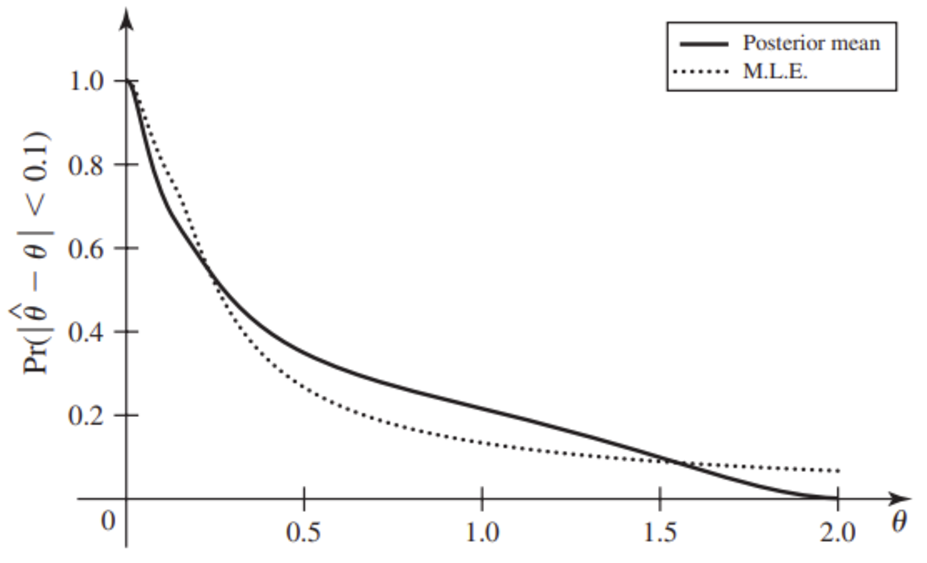
\includegraphics[scale=0.6]{figures/probability_curves_DeGroot8.1.pdf}
 \end{figure}
\end{frame}

\section{Qui-quadrado}

\begin{frame}{A distribuição qui-quadrado}
 \begin{defn}[Distribuição qui-quadrado]
 Dizemos que uma variável aleatória $Y$ tem distribuição~\textbf{qui-quadrado} com $m$ graus de liberdade quando
 \begin{equation}
 f_Y(y) = \frac{1}{2^{m/2}\Gamma(m/2)} y^{m/2 - 1}e^{-y/2}, \: y >0.
 \end{equation} 
 
 Vemos que $Y$ tem função geradora de momentos
\[\psi(t) = \left( \frac{1}{1-2t}\right)^{m/2}, t < 1/2 .\]
 \end{defn}
$E[Y] = ?$, $\vr(Y) =?$  
\end{frame}

\begin{frame}{Alguns resultados úteis}

\begin{theo}[Soma de variáveis aleatórias qui-quadrado]
Se $\rs$ são variáveis aleatórias independentes com graus de liberdade $m_i$, então $W = \sum_{i=1}^n X_i$ tem distribuição qui-quadrado com graus de liberdade $m =  \sum_{i=1}^n m_i$.
\end{theo}
\textbf{Prova}: Segue da soma de variáveis aleatórias Gama.

\begin{theo}[Distribuição do quadrado de uma variável aleatória Normal padrão]
Se $X \sim\operatorname{Normal}(0, 1)$, $Y = X^2$ tem distribuição qui-quadrado com $m=1$. 
\end{theo}
\textbf{Prova}: Escrever a acumulada de $Y$, diferenciar e usar a regra da cadeia.

\begin{obs}[Distribuição da soma de quadrados de normais padrão]
\label{rmk:sum_squares_standard_normal}
 Se $\rs$ são variáveis aleatórias Normal padrão, então $Z = \sum_{i=1}^n X_i^2$ tem distribuição qui-quadrado com $n$ graus de liberdade.
\end{obs}
\textbf{Prova}: Imediato dos dois últimos teoremas.

\end{frame}

\begin{frame}{Distribuição da variância amostral}
 Vamos a um exemplo motivador.
No caso Normal, quando $\mu$ é conhecida, temos o estimador de máxima verossimilhança para a variância:
\[ \hat{\sigma^2} = \frac{1}{n} \sum_{i=1}^n (X_i - \mu)^2. \]
Isso nos leva às duas próximas observações
\begin{obs}[Uma transformação linear do EMV]
 \begin{equation*}
  \frac{n\hat{\sigma^2}}{\sigma^2} \sim \operatorname{qui-quadrado}(n).
 \end{equation*}
\end{obs}
\textbf{Prova}: Notar que $Z_i = (X_i-\mu)/\sigma$ são Normal padrão e aplicar a observação~\ref{rmk:sum_squares_standard_normal}.

\begin{obs}[Distribuição do EMV da variância]
\label{rmk:sampling_distribution_normal_variance}
 \begin{equation*}
  \hat{\sigma^2} \sim \operatorname{Gama}\left(\frac{n}{2}, \frac{n}{2\sigma^2} \right).
 \end{equation*}

\end{obs}
\textbf{Prova}: Exercício 13 da seção 8.2 de DeGroot. 
\end{frame}

\begin{frame}{Quem comeu o meu queijo?}
 \begin{exemplo}[Concentração de ácido no queijo]
  Suponha que estamos interessados em medir a concentração de um certo ácido em pedaços de queijo produzidos por uma fábrica.
  Ao longo dos anos, grande acúmulo de dados permitiu afirmar que a distribuição populacional da concentração é Normal com parâmetros $\mu$ e $\sigma^2$.
  Suponha que amostramos $n$ pedaços e medimos as concentrações $\rs$.
  Então 
  \[ Y = \frac{1}{n}\sum_{i=1}^n |X_i-\mu|^2 \]
é uma medida de quanto estas amostras desviam da concentração típica $\mu$.
Suponha que uma diferença de concentração $u$ é o suficiente para dar gosto diferente ao queijo.
Podemos calcular $\pr(Y \leq u^2)$ para quantificar o risco de isso acontecer.
 \end{exemplo}

\end{frame}

\begin{frame}{O que aprendemos?}
\begin{itemize}

  \item[\faLightbulbO] Distribuição amostral;    
  
   ``Estatísticas e estimadores são variáveis aleatórias e têm distribuições amostrais''
  
  \item[\faLightbulbO] A distribuição qui-quadrado;
  
  ``A soma de quadrados de variáveis aleatórias gaussianas é um tipo especial de distribuição Gama''
  
  \item[\faLightbulbO] Avaliação probabilística de estimadores;
  
  ``Podemos utilizar a distribuição amostral para fazer afirmações sobre quantidades como $|\hat{\theta}-\theta|$''
  
  \end{itemize}
 \end{frame}

\begin{frame}{Leitura recomendada}
\begin{itemize}
 \item[\faBook] De Groot seções 8.1 e 8.2;
%  \item[\faBook] $^\ast$ Casella \& Berger (2002), seção 6.2.
%  \item[\faBook] $^\ast$ Schervish (1995), capítulo 7.
 \item {\large\textbf{Exercícios recomendados}}
 \begin{itemize}
  \item[\faBookmark] De Groot.
  \begin{itemize}
   \item Seção 8.1: exercícios 1, 2, 3 e 9;
   \item Seção 8.2: exercícios 4, 7, 10 e 13.
  \end{itemize}   
  \end{itemize}
 \end{itemize} 
\end{frame}

\section{Distribuição de média e variância amostrais}
\begin{frame}{Distribuição de média e variância amostrais}
 \begin{itemize}
  \item Distribuição conjunta de $\Sm$ e $\Sv$;
  \item No caso Normal, $\Sm \indep \Sv$ são idependentes!
  \item Distribuição t de Student.
 \end{itemize}
\end{frame}

\begin{frame}{Distribuição de $\Sm$ e $\Sv$}
 \begin{itemize}
  \item $\Sm \sim \operatorname{Normal}\left(\mu, \frac{\sigma^2}{n}\right)$;
  \item $\Sv \sim \operatorname{Gama}\left(\frac{n-1}{2},  \frac{n}{2\sigma^2}\right)$
 \end{itemize}
 \begin{figure}[!ht]
\label{fig:sample_moments_normal}
\begin{center}
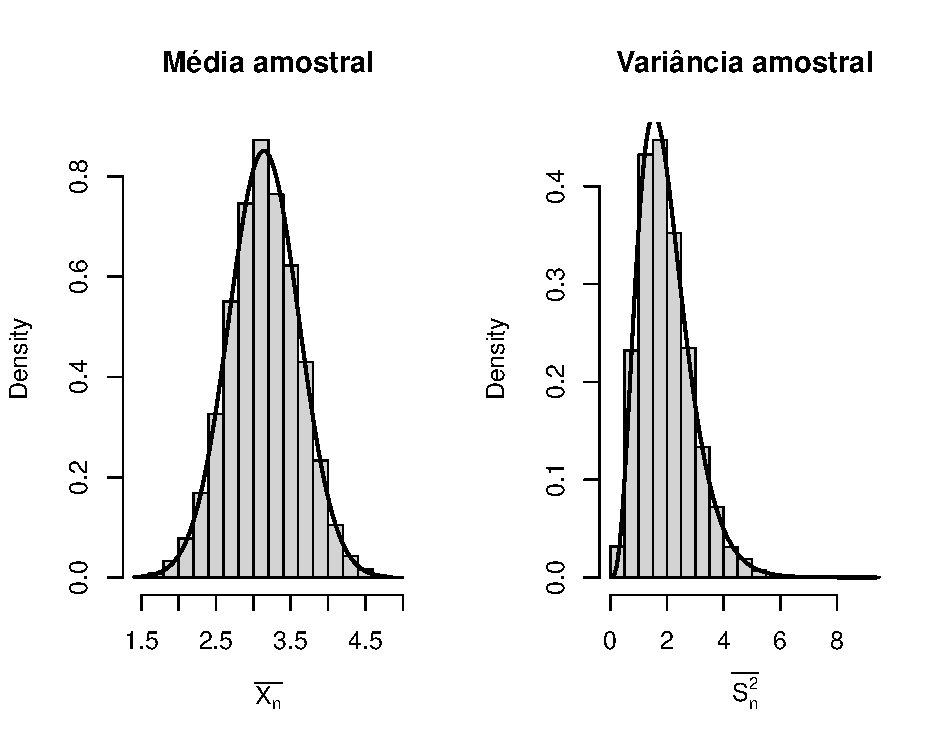
\includegraphics[scale=0.5]{figures/sample_moments_normal.pdf} 
\end{center} 
\end{figure} 
\end{frame}

\begin{frame}{Um Teorema importante}
 Aqui vamos ver um caso especial do Teorema de Basu\footnote{Debabrata Basu (1924--2001) foi um importante estatístico indiano.}, que fala que os dois primeiros momentos amostrais da distribuição Normal são independentes.
 \begin{theo}[Independência da média e variância amostrais na Normal]
 \label{thm:independence_sample_mean_variance_normal}
  Seja $\rs$ uma amostra aleatória de uma distribuição Normal com parâmetros $\mu$ e $\sigma^2$.
  Então a média amostral, $\Sm$ e a variância amostral, $\Sv$, são independentes.
  Ademais, $\Sm \sim \operatorname{Normal}\left(\mu, \frac{\sigma^2}{n}\right)$ e $\Sv \sim \operatorname{Gama}\left(\frac{n-1}{2},  \frac{n}{2\sigma^2}\right)$.
 \end{theo}
\textbf{Prova:} Troca de variáveis em duas dimensões; propriedades de matrizes ortogonais.
Ver Teorema 8.3.1 em DeGroot (prova na pág. 476).
\end{frame}

\begin{frame}{Exemplo}
 Suponha que queremos determinar o tamanho de amostra, $n$, de modo que os EMVs da média $\mu$ e do desvio padrão $\sigma$ estejam ``perto'' dos seus valores verdadeiros.
 Formalmente, queremos encontrar $n$ tal que
 \[ \pr\left( \left|\hat{\mu} - \mu\right| \leq \frac{1}{5}\sigma \: \text{\underline{e}} \: \left|\hat{\sigma}-\sigma\right| \leq  \frac{1}{5}\sigma \right) \geq \frac{1}{2} ,\]
 seja satisfeito.
\end{frame}

\begin{frame}{A distribuição $t$ de Student}
 Qual a distribuição de $\frac{\sqrt{n}\left(\Sm - \mu\right)}{\hat{\sigma}}$?
 A resposta é a distribuição t de ``Student''\footnote{William Sealy Gosset (1876--1937) foi um estatístico inglês que, em 1908, publicou o resultado acima sob o pseudônimo ``Student'', ou estudante/aluno.}
 
 \begin{defn}[A distribuição t]
 \label{def:Student_t_distribution}
  Considere duas variáveis aleatórias, $Y \sim\operatorname{Qui-quadrado}(m)$ e $Z \sim\operatorname{Normal}(0, 1)$ e defina a variável aleatória
  \[ X = \frac{Z}{\sqrt{\frac{Y}{m}}}. \]
 Dizemos que $X$  tem distribuição~\textbf{t de Student com $m$ graus de liberdade}. 
 Sabemos ainda que
 \[f_X(x) = \frac{\Gamma(\frac{m + 1}{2})}{\sqrt{m\pi}\Gamma(\frac{m}{2})} \left(1 + \frac{x^2}{m}\right)^{-\frac{m+1}{2}},\: x \in (-\infty, \infty). \]
 \end{defn}
Para $m>2$, $E[X] = 0$ (porquê?) e $\vr(X) = m/(m-2)$.
\end{frame}

\begin{frame}{Comparando a t com outras distribuições}
\begin{figure}[!ht]
 \begin{center}
  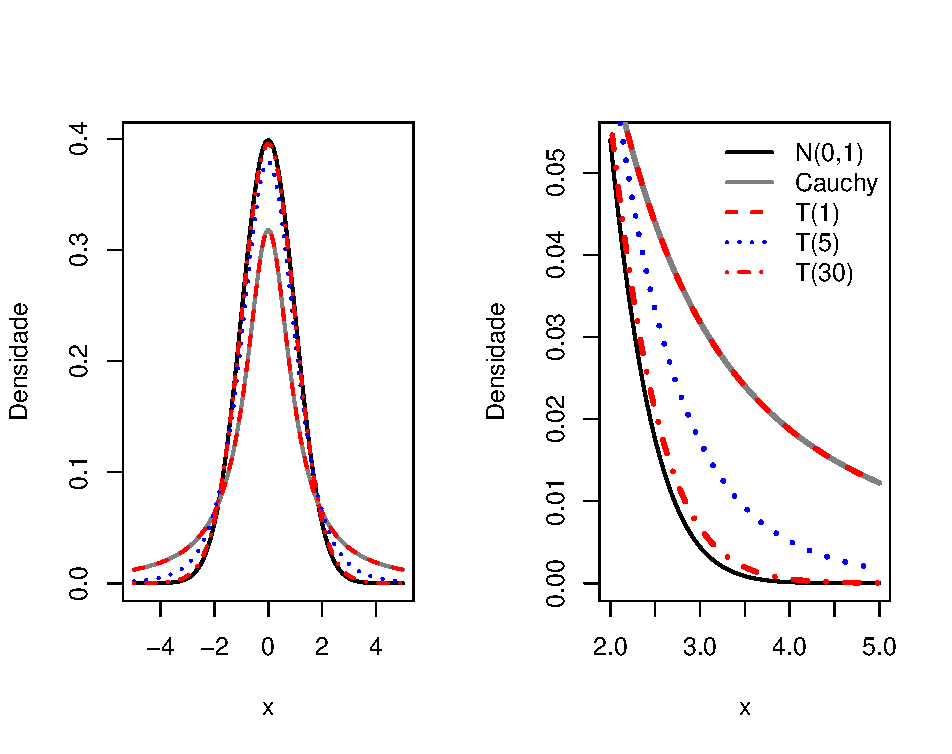
\includegraphics[scale=.6]{figures/comparacao_t_Student.pdf}
 \end{center}
\end{figure} 
\end{frame}

\begin{frame}{Um exemplo}
\begin{theo}[Distribuição amostral do estimador não-viesado da variância]
\label{thm:unbiased_variance_estimator_StudentT}
 Considere o estimador 
 \begin{equation*}
  \hat{\sigma}^\prime = \sqrt{\frac{\Delta^2}{n-1}},
 \end{equation*}
onde $\Delta^2 = \sum_{i=1}^n \left(X_i - \Sm\right)^2$.
Então 
\begin{equation*}
 \frac{\sqrt{n}\left(\Sm - \mu\right)}{\hat{\sigma}^\prime} \sim \operatorname{Student}(n-1).
\end{equation*}
\end{theo}
\textbf{Prova:}
Ver Teorema 8.4.2 em DeGroot.
Defina $Z = \sqrt{n}(\Sm - \mu)/\sigma$ e $Y = \Delta^2/\sigma^2$.
Então $Z \sim\operatorname{Normal}(0,1)$ e $Y\sim\operatorname{Qui-quadrado}(n-1)$.
Faça
\begin{equation}
 U = \frac{Z}{\sqrt{\frac{Y}{n-1}}} = \frac{\sqrt{n}(\Sm-\mu)}{\sqrt{\frac{\Delta^2}{n-1}}},
\end{equation}
e note que $U \sim \operatorname{T}(n-1)$  $\qed$
\end{frame}

\begin{frame}{O que aprendemos?}
\begin{itemize}

  \item[\faLightbulbO] Independência dos momentos amostrais da Normal;    
  
   ``Numa amostra aleatória Normal, $\Sm$ e $\Sv$ são independentes e $\Sm \sim \operatorname{Normal}\left(\mu, \frac{\sigma^2}{n}\right)$ e $\Sv \sim \operatorname{Gama}\left(\frac{n-1}{2},  \frac{n}{2\sigma^2}\right)$.''  
     
   \item[\faLightbulbO] A distribuição t de Student;
   
   ``A diferença padronizada entre a média amostral e a média populacional ($\mu$) tem distribuição t de Student, que não depende de $\sigma^2$''
    
  \end{itemize}
 \end{frame}

\begin{frame}{Leitura recomendada}
\begin{itemize}
 \item[\faBook] DeGroot seções 8.3 e 8.4;
%  \item[\faBook] $^\ast$ Casella \& Berger (2002), seção 6.2.
%  \item[\faBook] $^\ast$ Schervish (1995), capítulo 7.
 \item[\faForward] Próxima aula: DeGroot, seção 8.5;
 \item {\large\textbf{Exercícios recomendados}}
 \begin{itemize}
  \item[\faBookmark] DeGroot.
  \begin{itemize}
   \item Seção 8.3: exercício 8;
   \item Seção 8.4: derivar a densidade da Distribuição t de Student.
  \end{itemize}   
  \end{itemize}
 \end{itemize} 
\end{frame}

\section{Intervalos de confiança}
\begin{frame}{Intervalos de confiança}
 \begin{itemize}
  \item Intervalos de confiança;
  \item Caso normal: média;
  \item Intervalos de confiança unilaterais;
  \item Estatística pivotal.  
 \end{itemize}
\end{frame}

\begin{frame}{Intervalo de confiança para a média no caso Normal}
 Lembremos que 
 \begin{equation}
 U = \frac{\sqrt{n}(\Sm-\mu)}{\sqrt{\frac{\Delta^2}{n-1}}} \sim\operatorname{T}(n-1).
\end{equation}
Para $c>0$, podemos computar $\pr(-c < U < c) = \gamma$:
\begin{align*}
 &\pr\left(-c < \frac{\sqrt{n}(\Sm-\mu)}{\sqrt{\frac{\Delta^2}{n-1}}} < c\right) = \gamma,\\
 &\pr\left( \Sm - \frac{c\sigma^\prime}{\sqrt{n}} < \mu <  \Sm + \frac{c\sigma^\prime}{\sqrt{n}}\right) = \gamma,\\
 &T_{n-1}(c) - T_{n-1}(-c) = 2T_{n-1}(c) - 1 = \gamma.
\end{align*}
Concluímos que $c = F_T^{-1}\left(\frac{1 + \gamma}{2}; n-1\right)$.
\end{frame}

\begin{frame}{Definição de intervalo de confiança}
 O conceito de~\textbf{intervalo de confiança} é fundamental em Estatística e nas aplicações em Ciência.
 \begin{defn}[Intervalo de confiança]
  Seja $\bX = \{ \rs \}$ uma amostra aleatória, cada variável aleatória com p.d.f. $f(x\mid \theta)$, e considere uma função real $g(\theta)$.
  Sejam $A(\bX)$ e $B(\bX)$ duas estatísticas de modo que valha
  \begin{equation}
   \label{eq:confidence_interval}
   \pr\left\{A(\bX) < g(\theta) <  B(\bX)\right\} \geq \gamma.
  \end{equation}
Dizemos que $I(\bX) = (A(\bX), B(\bX))$ é um~\textbf{intervalo de confiança} de $100\gamma\%$ para $g(\theta)$.
Se a desigualdade for uma igualdade para todo $\theta \in \Omega$, dizemos que o intervalo é~\textbf{exato}.
 \end{defn}
\end{frame}

\begin{frame}{Revisitando o caso Normal}
No caso do intervalo de confiança para o parâmetro de média, temos 
$$\pr\left\{A(\bX) < g(\mu) <  B(\bX)\right\} \geq \gamma,$$
com $g(\mu) = \mu$  e 
\begin{align*}
 A(\bX) &= \Sm - \frac{c\sigma^\prime}{\sqrt{n}} = \Sm - \frac{c\sqrt{\sum_{i=1}^n \left(X_i - \Sm\right)^2}}{\sqrt{n(n-1)}},\\
 B(\bX) &= \Sm + \frac{c\sigma^\prime}{\sqrt{n}} = \Sm + \frac{c\sqrt{\sum_{i=1}^n \left(X_i - \Sm\right)^2}}{\sqrt{n(n-1)}}.
\end{align*}
\end{frame}

\begin{frame}{Interpretação de um intervalo de confiança}
 \textbf{ATENÇÃO:} a interpretação de um intervalo é crucial.
 Muita gente confunde o que um intervalo de confiança significa!
 \begin{obs}[Um intervalo de confiança não é uma afirmação sobre o(s) parâmetro(s)!]
  A afirmação probabilística da forma $\pr\left\{A(\bX) < g(\theta) <  B(\bX)\right\} = \gamma$ diz respeito à distribuição conjunta das variáveis aleatórias  $A(\bX)$ e $B(\bX)$ para um valor fixo de $\theta$ -- e, portanto, de $g(\theta)$.
 \end{obs}
 
 \begin{ideia}[Intervalos de confiança são procedimentos] 
 Como de costume na teoria ortodoxa (frequentista), o foco da construção de um intervalo confiança está em dar garantias probabilísticas~\textbf{com relação à \underline{distribuição dos dados}}.
 Dizer que $\pr\left\{A(\bX) < g(\theta) <  B(\bX)\right\} = \gamma$ é dizer que, se eu gerasse $M$ grande amostras aleatórias $\bX^{(1)}, \bX^{(2)}, \ldots, \bX^{(M)}$ de tamanho $n$ e construisse $M$ intervalos $I(\bX^{(1)}), I(\bX^{(2)}), \ldots, I(\bX^{(M)})$, eu esperaria encontrar:
 \begin{equation*}
  \frac{1}{M}\sum_{i=1}^M \mathbb{I}\left(g(\theta) \in I(\bX^{(1)}) \right) \approx \gamma.
 \end{equation*}
\end{ideia}

\end{frame}




\begin{frame}{O que aprendemos?}
\begin{itemize}

  \item[\faLightbulbO] Intervalos de confiança;    
  
   ``Um intervalo $(A(\bX), B(\bX))$  de confiança de $100\gamma\%$ para $g(\theta)$ é tal que $\pr\left[ A(\bX) < g(\theta) <  B(\bX) \right] \geq \gamma$'';
   
  \item[\faLightbulbO] Um intervalo de confiança é uma afirmação probabilística sobre~\textbf{as estatísticas} $A(\bX)$ e $B(\bX)$ a partir da~\textbf{distribuição conjunta dos dados};
     
%    \item[\faLightbulbO] ;
%    
%    ``''
  \end{itemize}
 \end{frame}

\begin{frame}{Leitura recomendada}
\begin{itemize}
 \item[\faBook] De Groot seção 8.5;
%  \item[\faBook] $^\ast$ Casella \& Berger (2002), seção 6.2.
%  \item[\faBook] $^\ast$ Schervish (1995), capítulo 7.
 \item[\faForward] Próxima aula: De Groot, seção 9.1;
 \item {\large\textbf{Exercícios recomendados}}
 \begin{itemize}
  \item[\faBookmark] De Groot.
  \begin{itemize}
   \item Seção 8.5: 1, 4 e 6.
  \end{itemize}   
  \end{itemize}
 \end{itemize} 
\end{frame}

\section{Testes de hipóteses I}
\begin{frame}{Testes de hipóteses}
 \begin{itemize}
  \item Hipótese nula e alternativa;
  \item Hipóteses simples e compostas;
  \item Região crítica e estatística teste;
  \item Função poder;
  \item Tipos de erro (I e II);
  \item P-valor;
   \end{itemize}
\end{frame}

\begin{frame}{Hipótese nula e alternativa}
 No teste de hipóteses estatísticas, identificamos partições do espaço de parâmetros que codificam as hipóteses de interesse.
 \begin{defn}[Hipótese nula e hipótese alternativa]
 \label{def:hypotheses}
  Considere o espaço de parâmetros $\Omega$ e defina $\Omega_0, \Omega_1 \subset \Omega$ de modo que $\Omega_0 \cup \Omega_1 = \Omega$ e $\Omega_0 \cap \Omega_1 = \emptyset$.
  Definimos
  \begin{align*}
   H_0 &:= \theta \in \Omega_0,\\
   H_1 &:= \theta \in \Omega_1.
  \end{align*}
Dizemos que $H_0$ é a~\textbf{hipótese nula} e $H_1$ é a~\textbf{hipótese alternativa}.

Se $\theta \in \Omega_1$, dizemos que~\textit{rejeitamos} a hipótese nula.
Por outro lado, se $\theta \in \Omega_0$ dizemos que~\textit{não rejeitamos} ou~\textit{falhamos em rejeitar} $H_0$.
 \end{defn}
\end{frame}

\begin{frame}{Exemplo}
Suponha que Palmirinha recebeu uma carta da Associação Nacional da Pamonha Gourmet (ANPG), dizendo que a pamonha deve ter, no mínimo, 7 mg/L de concentração de amido.
Supondo que a concentração de amido tenha distribuição Normal com parâmetros $\mu$ (desconhecido) e $\sigma^2$ (conhecido), Palmirinha rabisca num papel:
  \begin{align*}
   H_0 &:\mu \in [7, \infty),\\
   H_1 &: \mu \in (0, 7).
  \end{align*}
\end{frame}

\begin{frame}{Hipóteses simples e compostas}
 Dependendo do tipo de partição do espaço de parâmetros, as hipóteses recebem classificações diferentes.
 \begin{defn}[Hipótese simples e hipótese compostas]
 \label{def:hypotheses_typesI}
  Dizemos que uma hipótese $H_i$, é~\textbf{simples}, se $\Omega_i = \{ \theta_i \}$, isto é, se a partição correspondente é um ponto. 
  Uma hipótese é dita~\textbf{composta} se não é simples.
 \end{defn}
 
 \begin{exemplo}[Hipótese simples sobre a média]
  Suponha que estamos estudando o efeito de uma droga na redução da pressão arterial.
  Modelamos esta redução como uma variável aleatória $X$ com esperança $E[X] =: \theta$.
  É costumaz testar a hipótese $H_0 : \theta = 0$, que chamamos, especificamente nesse caso, de ``hipótese de efeito nulo''.
 \end{exemplo}
\end{frame}

\begin{frame}{Hipótese unilateral e hipótese bilateral}
 Em analogia com os intervalos de confiança, também podemos entender as hipóteses como sendo unilaterais ou bilaterais.
 \begin{defn}[Hipótese unilateral e hipótese bilateral]
  \label{def:hypotheses_typesII}
  Uma hipótese da forma $H_0 : \theta \leq \theta_0$ ou $H_0 : \theta \geq \theta_0$ é dita~\textit{unilateral} (``\textit{one-sided}''), enquanto hipóteses da forma $H_0 : \theta \neq \theta_0$ são ditas bilaterais (``\textit{two-sided}'').
 \end{defn}
 
 \begin{obs}[Hipóteses bilaterais como consequência de $H_0$ simples]
 Se $H_0$ é simples, a hipótese alternativa $H_1$ será, em geral, bilateral.  
 \end{obs}
\end{frame}

\begin{frame}{Região crítica: exemplo motivador}
 \begin{exemplo}[Teste para a média de uma Normal com variância conhecida]
  \label{ex:test_normal_mean_knownVar}
  Suponha que $\bX = \{ \rs \}$ é uma amostra aleatória de uma Normal com média $\mu$ e variância $\sigma^2$ conhecida.
  Queremos testar a hipótese
  \begin{align*}
   H_0 &: \mu = \mu_0\\
   H_1 &: \mu \neq \mu_0.
  \end{align*}
  Intuitivamente, queremos rejeitar $H_0$ se $\Sm$ está longe de $\mu_0$.
  Para isso definimos
  \[ S_0 := \left\{ \bx: -c \leq \Sm - \mu_0 \leq c \right\}, \]
  de modo que $S_1 = S_0^C$. 
  Então, seguimos o procedimento:
      \begin{align*}
   \bX \in S_1 &\implies \text{rejeitar}\: H_0,\\
   \bX \in S_0 &\implies \text{não\:rejeitar}\: H_0.\\
  \end{align*}
 \end{exemplo}
\end{frame}

\begin{frame}{Região crítica e região de rejeição}
 Uma maneira mais simples de expressar o procedimento acima é definir $T := \left|\Sm - \mu_0\right|$ e rejeitar $H_0$ se $T \geq c$.
 \begin{defn}[Região crítica]
 \label{def:critical_region}
  O conjunto 
   \[ S_1 := \left\{ \bx:  \left|\Sm - \mu_0\right| \geq c \right\}, \]
   é chamado de~\textbf{região crítica} do teste.
 \end{defn}
 
Analogamente, considere a estatística $T = r(\bX)$ e tome $R \subseteq \mathbb{R}$. 
Então podemos definir
\begin{defn}[Região de rejeição]
\label{def:rejection_region}
Se $R \subseteq \mathbb{R}$ é tal que dizemos que ``rejeitamos $H_0$ se $T \in R$'', então $R$ é chamada uma~\textbf{região de rejeição} para a estatística $T$ e o teste associado.
\end{defn}
\end{frame}

\begin{frame}{Dividindo o espaço amostral e o espaço de parâmetros}
 Começamos com uma observação:
 \begin{obs}[Correspondência entre região crítica e região de rejeição]
 Podemos relacionar os conceitos de região crítica e região de rejeição notando queremos
   \[ S_1 := \left\{ \bx:  r(\bx) \in R \right\}. \]
\end{obs}

\begin{ideia}[Dividindo o espaço amostral e o espaço de parâmetros]
\label{idea:splitting_sample_space_parameter_spaces}
 Suponha que temos um modelo estatístico dado pela distribuição $f(x\mid\theta)$, com $x \in \mathcal{X}$ e $\theta \in \Omega$.
 Desta forma, uma amostra aleatória $\bX = \{ \rs\}$ mora em $\mathcal{X}^n$.
 Para formular uma hipótese estatística, estabelecemos uma partição do espaço de parâmetros $\Omega$ em $\Omega_0$ e $\Omega_1$ disjuntos.
 Isto, por sua vez, induz uma partição $S_0, S_1 \in \mathcal{X}^n$.
 Estes objetos, embora, relacionados,~\textbf{não são a mesma coisa}.
 Por exemplo, nós observamos se $\bX \in S_0$ ou $\bX \in S_1$, mas raramente ``observamos'' se $\theta \in \Omega_0$ ou $\theta \in \Omega_1$.
\end{ideia}
\end{frame}

\begin{frame}{Função poder}
 Nossa capacidade de rejeitar $H_0$ depende do valor de $\theta \in \Omega$.
 Esta dependência é capturada pela função poder.
 \begin{defn}[Função poder]
 \label{def:power_function}
  Seja $\delta$ um procedimento de aceitação/rejeição como visto anteriormente.
  A~\textbf{função poder} é definida como 
  \begin{equation}
   \label{eq:power_function}
   \pi(\theta\mid \delta) := \pr\left(\bX \in S_1 \mid \theta\right) = \pr\left(T \in R \mid \theta\right), \theta \in \Omega.
  \end{equation}
 \end{defn}
Idealmente, queremos $\pi(\theta \mid \delta) = 1$ para $\theta \in \Omega_1$ (por quê?).
\end{frame}

\begin{frame}{A função poder de um teste para a média da Normal}
 Considere a situação em que $\rs$ vêm de uma Normal com média $\mu$, desconhecida, e variância $\sigma^2$, conhecida.
 \begin{exemplo}[Função poder no teste para média da Normal ($\sigma^2$ conhecida)]
 \label{ex:power_function_normal_mean_test}
  Lembrando que $T = |\Sm - \mu_0|$, e tomando $\delta$ como o procedimento descrito acima, escrevemos
  \begin{align*}
   \pi(\mu \mid \delta) &= \pr(T \in R \mid \mu),\\
   &= \pr\left(\Sm \geq \mu_0 + c \mid \mu \right) + \pr\left( \Sm \leq \mu_0 -c \mid \mu \right),\\
   &= \left\{ 1 - \Phi\left(\sqrt{n} \frac{\mu_0 + c -\mu}{\sigma}\right) \right\} + \Phi\left(\sqrt{n} \frac{\mu_0 - c -\mu}{\sigma}\right). 
  \end{align*}
 \end{exemplo}
\end{frame}

\begin{frame}{Pelo poder da pamonha...}
\begin{figure}
 \begin{center}
  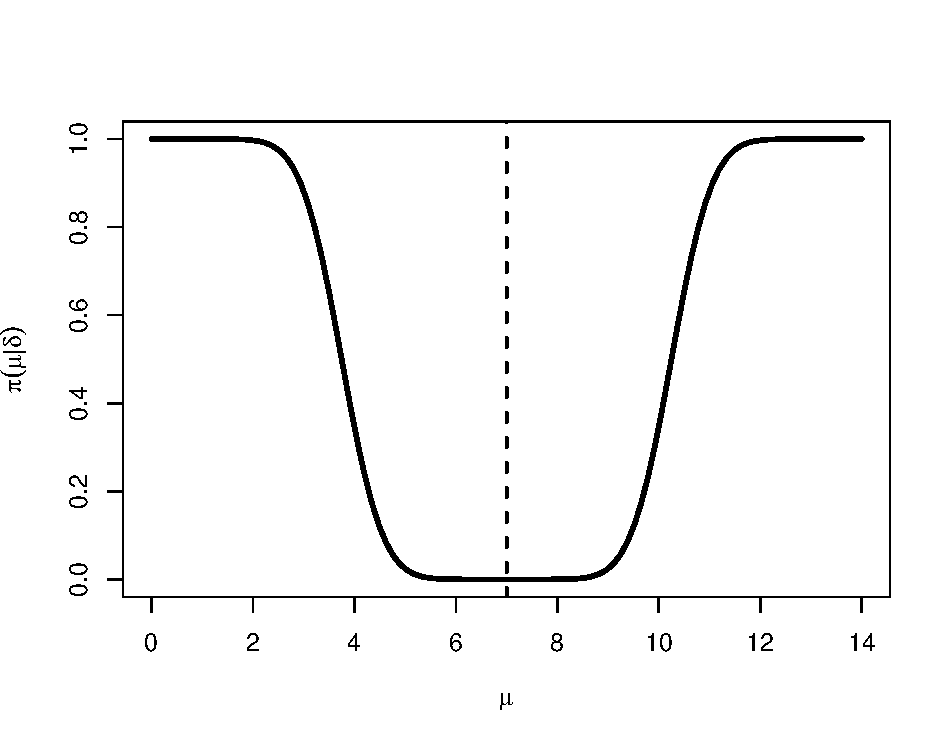
\includegraphics[scale=0.6]{figures/poder_palmirinha.pdf}
 \end{center}
\end{figure} 
\end{frame}
 
\begin{frame}{Tipos de Erro}
 Quando testamos uma hipótese, nunca estamos livres de cometer um erro.
 É conveniente classificar os possíveis erros em duas categorias.
 \begin{defn}[Tipos de erros]
 \label{def:error_types}
 \begin{center}
  \begin{tabular}{cc}
   Nome & Erro cometido\\
   \hline
   Erro tipo I & Rejeitar $H_0$ quando ela é~\textbf{verdadeira}.\\
   Erro tipo II & Falhar em rejeitar $H_0$ quando ela é~\textbf{falsa}.\\
   \hline
  \end{tabular}
 \end{center}  
 \end{defn}
Isto nos leva a concluir que
\begin{center}
  \begin{tabular}{ccl}
   Situação & Quantidade & Interpretação\\
   \hline
    $\theta \in \Omega_0$ & $\pi(\theta \mid \delta)$ & $\pr(\text{Erro\: tipo\: I})$ \\
    $\theta \in \Omega_1$ & $1-\pi(\theta \mid \delta)$& $\pr(\text{Erro\: tipo\: II})$\\
   \hline
  \end{tabular}
\end{center} 
 \end{frame}

\begin{frame}{Balanceando um teste}
 Idealmente, gostaríamos de um teste $\delta$ para o qual as probabilidades de erro fossem as menores possíveis. 
 Infelizmente, em geral, diminuir o erro tipo I implica aumentar o erro tipo II. 
%  Tome, por exemplo, um teste $\delta_0$ que~\textbf{nunca} rejeita $H_0$, terá $\pi(\theta \mid \delta_0 = 0$ para todo $\theta \in \Omega_0$, o que é bom, mas também terá  $\pi(\theta \mid \delta_0 = 0$ para $\theta \in \Omega_1$, o que é bem ruim.

 Em geral, precisamos encontrar um equilíbrio entre os tipos de erros.
 \begin{ideia}[Encontrando um balanço entre erro tipo I e tipo II]
 \label{idea:balancing_typeI_and_typeII}
  Tome $0 < \alpha_0 < 1$.
  Nós construímos o procedimento $\delta^\ast$ de modo que
  \begin{equation}
  \label{eq:test_maxsize}
   \pi(\theta \mid \delta^\ast) \leq \alpha_0, \: \forall\: \theta \in \Omega.
  \end{equation}
 Então, entre todos os testes que satisfazem~(\ref{eq:test_maxsize}), buscamos o teste que tenha $\pi(\theta \mid \delta^\ast)$ máxima em $\theta \in \Omega_1$.
 \end{ideia}
\end{frame}
 
 
\begin{frame}{Tamanho de um teste}
 \begin{defn}[Tamanho/nível de um teste]
 \label{def:size_test}
 Dizemos que um teste, $\delta$, tem~\textbf{tamanho} ou~\textbf{nível de significância} $\alpha(\delta)$, com 
 \begin{equation*}
  \alpha(\delta) := \sup_{\theta \in \Omega_0} \pi(\theta \mid \delta).
 \end{equation*}
 \end{defn}
Um teste que atende à condição anterior (\ref{eq:test_maxsize}) tem que tamanho?

\begin{obs}[Tamanho de um teste com $H_0$ simples]
 Se $H_0$ é simples, então $\alpha(\delta) = \pi(\theta_0 \mid \delta)$.
\end{obs}

\end{frame}

\begin{frame}{Um exemplo}
 \begin{exemplo}[Teste para o parâmetro de uma uniforme]
 \label{ex:test_uniform_parameter}
  Suponha que $\rs$ tem distribuição Uniforme em $[0, \theta]$, com $\theta$ desconhecido, e que aventamos as seguintes hipóteses:
  \begin{align*}
   H_0:&\: 3 \leq \theta \leq 4, \\
   H_1:&\:  \theta < 3 \:\text{ou}\: \theta > 4
  \end{align*}
  Lembre que $\emv = \max\{\rs\}$ e suponha que temos um teste $\delta$ da forma  
   \begin{center}
  \begin{tabular}{cc}
   Condição & Ação \\
   \hline
   $\emv \notin (2.9, 4)$ & Rejeitar $H_0$ \\
   $\emv \in (2.9, 4)$ & Falhar em rejeitar $H_0$.\\
   \hline
  \end{tabular}
 \end{center}  
 \end{exemplo}
\begin{itemize}
 \item Qual a região de rejeição para $\delta$?
 \item Como escrever $\pi(\theta \mid \delta)$?
 \item Qual o tamanho de $\delta$?
\end{itemize}
\end{frame}

\begin{frame}{Construindo um teste com o tamanho adequado}
 Em geral, sempre conseguimos construir um teste que tenha o tamanho desejado.
 \begin{obs}[Construindo um teste de tamanho $\alpha_0$]
  Se $T = r(\bX)$ é uma estatística, podemos quase sempre encontrar $c$ tal que valha
  \begin{equation}
   \label{eq:size_test_statistic}
   \sup_{\theta \in \Omega_0} \pr\left(T \geq c \mid \theta \right) \leq \alpha_0,
  \end{equation}
  ou seja, encontrar $c$ tal que $\delta$ tenha tamanho (ou nível de significância) $\alpha_0$.
 \end{obs}
\end{frame}

\begin{frame}{O p-valor}
Começamos com uma observação:
\begin{obs}[Testes são decisões binárias]
 Um teste de hipótese reduz a informação contida nos dados a uma decisão binária: rejeitar ou não $H_0$. 
 Se observamos $T = c + 10^{-10}$ ou $T = c + 10^{10}$, tomamos a~\textit{mesma decisão} de rejeitar $H_0$ ao nível $\alpha_0$.
\end{obs} 
Ao invés disso, podemos reportar o maior nível de significância que ainda levaria à rejeição de $H_0$.
\begin{defn}[O p-valor]
 \label{def:pvalue}
 Para cada $t$, seja $\delta_t$ o teste que rejeita $H_0$ se $T \geq t$.
 Então, quando $T = t$, o~\textbf{p-valor} vale
 \begin{equation}
   p(t) := \sup_{\theta \in \Omega_0} \pi(\theta \mid \delta_t) = \sup_{\theta \in \Omega_0} \pr\left(T \geq t \mid \theta \right),
 \end{equation}
ou seja, o p-valor é o tamanho do teste $\delta_t$.
\end{defn}
\end{frame}

\begin{frame}{Exemplo: tá me enganando, parceiro?}
Vamos voltar a uma pergunta não respondida lá no início do curso.
Suponha que você encontre um ``artista'' de rua, que joga uma moeda e pede para as pessoas apostarem se vai dar cara ou coroa.
Conhencendo estatística e probabilidade, você decide (i) observar o jogo à distância para coletar alguns dados (ii) fazer algumas contas para ver se vale a pena apostar.
 \begin{pergunta}[Esta moeda é justa? cont. I]
 \label{ex:moeda_justa_reborn}
  Suponha que uma moeda tenha sido lançada dez vezes, obtendo o seguinte resultado:
  \begin{equation*}
   KKKCKCCCKC
  \end{equation*}
\begin{itemize}
 \item[a)] Esta moeda é justa?
 \item[b)] Quanto eu espero ganhar se apostar R\$ 100,00 que é justa? 
\end{itemize}
 \end{pergunta}
 Hoje vamos dar uma resposta parcial à pergunta a).
\end{frame}

\begin{frame}{O que aprendemos?}
\begin{itemize}

  \item[\faLightbulbO] Hipóteses nula e alternativa, simples e composta;    
  \item[\faLightbulbO] Região crítica e região de rejeição;
  \item[\faLightbulbO] Função poder;
  
  ``O poder de um teste é a probabilidade de rejeitarmos $H_0$ caso ela seja falsa''
  
  \item[\faLightbulbO] Erro tipo I e tipo II;
  \begin{itemize}
   \item Tipo I: Rejeitar erroneamente $H_0$;
   \item Tipo II: Falhar em rejeitar $H_0$ quando ela é falsa.
  \end{itemize}
  \item[\faLightbulbO] P-valor;
  
  ``O p-valor pode ser interpretado como a probabilidade, sob $H_0$, de observarmos uma estatística tão ou mais extrema do que aquela que foi observada''
  \end{itemize}
 \end{frame}

\begin{frame}{Leitura recomendada}
\begin{itemize}
 \item[\faBook] DeGroot seção 9.1;
 \item[\faBook] $^\ast$ DeGroot seções 9.2 e 9.3.
%  \item[\faBook] $^\ast$ Schervish (1995), capítulo 7.
%  \item[\faBook] $^\ast$ Casella \& Berger (2002), seção 9.2.
 \item[\faForward] Próxima aula: DeGroot, seção 9.1 (razão de verossimilhanças);
 \item {\large\textbf{Exercícios recomendados}}
 \begin{itemize}
  \item[\faBookmark] DeGroot.
  \begin{itemize}
   \item Seção 9.1: 3, 8 e 13.
   \item $^\ast$ Seção 9.1: 19 e 21.
  \end{itemize}   
  \end{itemize}
 \end{itemize} 
\end{frame}

\section{Testes de hipóteses II}
\begin{frame}{Razões de verossimilhanças}
 \begin{itemize}
   \item Intervalos de confiança e testes;
   \item Razões de verossimilhanças
   \end{itemize}
\end{frame}

\begin{frame}{Intervalos de confiança $\equiv$ testes}
 De posse de um intervalo de confiança, podemos testar hipóteses sobre uma função dos parâmetros, $g(\theta)$, como mostra o seguinte teorema:
 \begin{theo}[Intervalos de confiança e testes são equivalentes]
 \label{thm:CIs_are_tests}
  Suponha que dispomos de dados $\bX = \{ \rs \}$ com f.d.p. comum $f(x \mid \theta)$, e estamos interessados em testar as hipóteses:
  \begin{align*}
   H_0 &: g(\theta) = g_0, \\
   H_1&: g(\theta) \neq g_0,
  \end{align*}
de modo que existe um teste $\delta_{g_0}$ com nível $\alpha_0$ destas hipóteses. 
Para cada $\bX = \bx$, defina
\[ w(\bx) = \left\{g_0: \delta_{g_0} \text{\:não\: rejeita\:} H_0\text{\:dado\:que\:} \bX = \bx \right\}.\]
Fazendo o nível de confiança do intervalo $\gamma = 1 -\alpha_0$, temos 
\[ \pr\left(g(\theta_0) \in w(\bX) \mid \theta = \theta_0 \right)  \geq \gamma,\: \forall \theta_0 \in \Omega. \]
 \end{theo}
\textbf{Prova:} Notar que $\pr\left(\delta_{g_0} \text{\: não\: rejeita\:} H_0 \mid \theta = \theta_0\right) \geq \alpha_0 = 1-\gamma$ e concluir que $w(\bX)$ é uma região de crítica para $\delta_{g_0}$.
Ver Teorema 9.1.1 de DeGroot.
\end{frame}

\begin{frame}{Conjunto de confiança}
 O conjunto $w(\bX)$ definido acima pode ser entendido como um conjunto de confiança para $g(\theta)$.
 \begin{defn}[Conjunto de confiança]
 \label{def:confidence_set}
  Se um conjunto aleatório $w(\bX)$ satisfaz 
  \[\pr\left(g(\theta_0) \in w(\bX) \mid \theta = \theta_0 \right)  \geq \gamma, \]
  para todo $\theta_0 \in \Omega$, então chamamos $w(\bX)$ de um~\textbf{conjunto de confiança} para $g(\theta)$.
 \end{defn}
 Isso nos leva ao seguinte teorema
 \begin{theo}[Testando hipóteses a partir de conjuntos de confiança]
 \label{thm:testing_hypotheses_confidence_sets}
  Suponha que dispomos de dados $\bX = \{ \rs \}$ com f.d.p. comum $f(x \mid \theta)$ e que $w(\bX)$ é um conjunto de confiança para uma função de interesse $g(\theta)$. 
  Então para todo valor $g_0$  assumido por $g(\theta)$ existe um teste $\delta_{g_0}$, de nível $\alpha_0$ que rejeita $H_0: g(\theta) = g_0 $ se e somente se $g(\theta_0)  = g_0 \notin w(\bX)$.
 \end{theo}
 \textbf{Prova:} Trivial.
 Ver DeGroot, Teorema 9.1.2.
\end{frame}

\begin{frame}{Exemplo}
 Vamos aplicar os conceitos discutidos ao caso Normal com variância conhecida.
 \begin{exemplo}[Teste para média da Normal com variância conhecida]
 \label{ex:test_normal_mean}
  Suponha que $\bX = \{ \rs \}$ formam uma amostra aleatória de uma distribuição Normal com média $\mu$ e variância $\sigma^2$, conhecida.
  Considere testar a hipótese
  \begin{align*}
   H_0 &:  \mu = \mu_0, \\
   H_1&: \mu \neq \mu_0.
  \end{align*}
  Seja $\alpha_0 = 1-\gamma$. 
  Lembre-se de que o teste de tamanho $\alpha_0$, $\delta_{\mu_0}$ é rejeitar $H_0$ se $|\Sm-\mu_0| \geq c$, $c := \Phi^{-1}\left(1-\alpha_0/2\right)\sigma\sqrt{n}$.
  Esta última desigualdade pode ser manipulada algebricamente para obter o intervalo de confiança exato
  $$ (A(\bX), B(\bX)) = \left( \Sm - c, \Sm + c\right), $$
  de modo que $\pr(A(\bX) < \mu_0 < B(\bX) | \mu = \mu_0) = \gamma$.
 \end{exemplo}
\end{frame}

\begin{frame}{Testes unicaudais e bi-caudais}
 Da mesma forma que intervalos de confiança podem ser uni- ou bilaterais. 
 Considere testar a hipótese
  \begin{align*}
   H_0 &:  g(\theta) \geq g_0, \\
   H_1&: g(\theta) < g_0.
  \end{align*}
Podemos testar esta hipótese a partir de um intervalo de confiança da forma $I_l = (A(\bX), \infty)$: se $g(\theta) \notin I_l$ então rejeitamos $H_0$.  
\end{frame}

\begin{frame}{Testes de razão de verossimilhanças}
 Considere testar 
  \begin{align*}
   H_0 &:  \theta \in \Omega_0, \\
   H_1&:  \theta \in \Omega_1. 
  \end{align*}
Em certas situações, podemos utilizar a função de verossimilhança para quantificar a evidência em favor de $H_0$.
\begin{defn}[Teste de razão de verossimilhanças]
 \label{def:LRT}
 A estatística
 \[ \Lambda(\bx) = \frac{\sup_{\theta \in \Omega_0} f_n(\bx \mid \theta) }{\sup_{\theta \in \Omega} f_n(\bx \mid \theta)}, \]
 é chamada uma~\textbf{estatística de razão de verossimilhanças}.
 Um~\textbf{um teste de razão de verossimilhanças}, $\delta_k$ é um teste que rejeita $H_0$ se $\Lambda(\bx) \leq k$ para uma constante $k$.
\end{defn}
\end{frame}

\begin{frame}{Teste de razão de verossimilhanças para a binomial}
\begin{exemplo}[Teste de razão de verossimilhanças para uma hipótese simples]
\label{ex:LRT_simple_hypothesis}
 Suponha que $\rs$ são uma amostra aleatória de uma distribuição Bernoulli com parâmetro $p$.
 Assim, temos $Y = \sum_{i=1}^n X_i$ e $Y~\operatorname{Binomial}(n, p)$.
 Considere testar a hipótese $H_0 :  p  = p_0, H_1:  p  \neq p0$.  
 Depois de observarmos $Y = y$, a função de verossimilhança é
 \[ f(\bx \mid p) = \pr(Y = y\mid p) = \binom{n}{y} p^y (1-p)^{n-y}. \]
 Como neste exemplo $\Omega_0 = \{p_0\}$ e $\Omega_1 = (0, 1)\setminus\{p_0\}$,
 \begin{equation*}
  \Lambda(\bx) = \frac{p_0^y (1-p_0)^{n-y}}{\sup_{p \in (0,1)}  p^y (1-p)^{n-y}}.
 \end{equation*}
O supremo no denominador é atingido no EMV, $\hat{p} = y/n$, de modo que
 \begin{equation*}
  \Lambda(\bx) = \left(\frac{np_0}{y}\right)^{y} \left(\frac{n(1-p_0)}{n-y}\right)^{n-y}.
 \end{equation*}
 Para mais detalhes, ver código no repositório do curso.
\end{exemplo} 
\end{frame}

\begin{frame}{Um teorema útil}
 Sob certas condições de regularidade, podemos fazer afirmações sobre a distribuição assintótica de $\log\Lambda(\bX)$.
 \begin{theo}[Teorema de Wilks\footnote{Em homenagem a Samuel Wilks (1906-1964), matemático estadounidense.}]
 \label{thm:Wilks}
  Suponha que temos um espaço de parâmetros com $k$ coordenadas, $\theta = (\theta_1, \theta_2, \ldots, \theta_k)$ e desejamos testar a hipótese (simples) da forma
   \begin{align*}
   H_0 &:  \theta_j = \theta_0^{j}, j = 1, 2, \ldots, k, \\
   H_1 &:  \theta_j \neq \theta_0^{j}, j = 1, 2, \ldots, k. 
  \end{align*}
  Então, sob condições de regularidade, temos que, à medida que $n \to \infty$,
  \begin{equation*}
   -2\log\Lambda(\bx) \xrightarrow{\text{d}} \chi^{2} (k), 
  \end{equation*}
 \end{theo}
\textbf{Prova:} Avançada, não será dada aqui.
Ver Teorema 9.1.4 de DeGroot.
Para a demonstração, ver Teorema 7.125 de Schervish (1995).
\end{frame}

\begin{frame}{O que aprendemos?}
\begin{itemize}

  \item[\faLightbulbO] Intervalos de confiança podem ser utilizados para testar hipóteses;
  \item[\faLightbulbO] Testes podem ser bicaudais ($1-\alpha_0/2$) quando unicaudais ($(1 + \alpha_0)/2)$;
  \item[\faLightbulbO] Razões de verossimilhanças
  
  ``A razão entre o supremo da função de verossimilhança tomado no espaço em que $H_0$ é verdadeira ($\Omega_0$) e o mesmo supremo tomado sobre todo o espaço de parâmetros ($\Omega$)''
  
  \item[\faLightbulbO] Teorema de Wilks; 
  
  ``À medida que o tamanho de amostra aumenta, menos duas vezes o logaritmo da razão de verossimilhanças tende em distribuição para uma Qui-quadrado com $k$ graus de liberdade''
  \end{itemize}
 \end{frame}

\begin{frame}{Leitura recomendada}
\begin{itemize}
 \item[\faBook] DeGroot seção 9.1;
 \item[\faBook] $^\ast$ Schervish (1995), capítulos 4.5.5 e 7.5 .
 \item[\faBook] $^\ast$ Casella \& Berger (2002), seção 8.2.
 \item[\faForward] Próxima aula: DeGroot, seção 9.5;
 \end{itemize} 
\end{frame}

\section{Teste t de Student}
\begin{frame}{Teste t (de Student)}
 \begin{itemize}
   \item Teste não-viesado;
   \item O teste t (unilateral e bilateral);
   \item Teste t pareado;
   \item Teste t para duas amostras;
   \begin{itemize}
    \item Variâncias iguais (homogeneidade);
    \item Variâncias proporcionais.
   \end{itemize}
   \item Propriedades e exemplos;
   \end{itemize}
\end{frame}

\begin{frame}{Teste não-viesado}
 Em analogia com o conceito de estimador não-viesado, podemos também classificar testes de hipótese em viesados ou não-viesados.
 \begin{defn}[Teste não viesado]
 \label{def:unbiased_tests}
  Suponha que desejamos testar a hipótese
  \begin{align*}
   H_0 &: \theta \in \Omega_0, \\
   H_1&:  \theta \in \Omega_1. 
  \end{align*}
  através do teste $\delta$.
  Dizemos que $\delta$ é~\textbf{não-viesado} se (e somente se) para $\theta \in \Omega_0$ e $\theta^\prime \in \Omega_1$, vale 
  \[ \pi(\theta \mid \delta) \leq   \pi(\theta^\prime \mid \delta),\]
  ou seja, se a~\textit{função poder} é pelo menos tão grande no espaço onde $H_0$ é falsa ($\Omega_1$) quanto no espaço em que $H_0$ é verdadeira ($\Omega_0$). 
 \end{defn}
\end{frame}

\begin{frame}{Teste t: motivação}
 Suponha que estamos interessados em testar hipóteses sobre a média ($\mu$) de uma distribuição Normal quando a variância ($\sigma^2$) é desconhecida.
 Sabemos que é possível encontrar uma quantidade pivotal $(\Sm-\mu)/\hat{\sigma}^\prime$ tal que é possível construir um intervalo de confiança para $\mu$ da forma $\Sm - c\hat{\sigma}^\prime/\sqrt{n}, \Sm + c\hat{\sigma}^\prime/\sqrt{n}$, onde $c = T^{-1}(\gamma; n-1)$ é a f.d.a. inversa de uma distribuição t de Student com $n-1$ graus de liberdade.
 
 \begin{pergunta}[Como falar sobre $\mu$ quando ambas $\mu$ e $\sigma^2$ são desconhecidas?]
 \label{qst:unknown_mean_and_variance}
  Suponha que Palmirinha esteja interessada em testar a hipótese de que a média da concentração de amido na sua pamonha seja maior que $\mu_0 = 7 mg/L$, ou seja,
    \begin{align*}
   H_0 &: \mu \geq \mu_0, \\
   H_1&:  \mu < \mu_0,
  \end{align*}
  mas ela desconhece a variância do processo, $\sigma^2$.
  Como testar hipóteses sobre $\theta = (\mu, \sigma^2)$?
 \end{pergunta} 
\end{frame}

\begin{frame}{Exemplo}
 Palmirinha pode começar computando a estatística 
 \begin{equation*}
  U:= \sqrt{n}\frac{\Sm-\mu_0}{\hat{\sigma}^\prime},
 \end{equation*}
onde $\hat{\sigma}^\prime = \sqrt{\sum_{i=1}^n (X_i - \Sm)^2/(n-1)}$ como já estudado.
A partir daí, pode construir um teste $\delta_c$ que rejeita $H_0$ se $U \leq c$, para uma constante real $c$ definida.
\begin{obs}[A distribuição de $U$ sob $H_0$]
 Quando $H_0$ é verdadeira, em particular, quando $\mu = \mu_0$, $U$ tem distribuição t de Student com $n-1$ graus de liberdade, não importando o valor de $\sigma^2$.
 Isto é, $U$ é pivotal.
\end{obs}
\end{frame}


\begin{frame}{Caracterizando o teste t}
\begin{defn}[Teste t]
\label{def:Student_t_test}
Um teste $\delta_c$ que rejeita $H_0$ se $U\geq c$ (equiv. $U \leq c$), com $c = T^{-1}(1-\alpha_0; n-1)$ é chamado um teste t (unicaudal) de tamanho $\alpha_0$.
\end{defn}
\begin{theo}[Propriedades do teste t]
Suponha que $\delta_c$ rejeita $H_0$ se $U\geq c$.
Então
\begin{itemize}
 \item [i)] $\mu = \mu_0 \implies \pi(\mu, \sigma^2 \mid \delta_c) = \alpha_0$;
 \item [ii)] $\mu < \mu_0 \implies \pi(\mu, \sigma^2 \mid \delta_c) < \alpha_0$;
 \item [iii)] $\mu > \mu_0 \implies \pi(\mu, \sigma^2 \mid \delta_c) > \alpha_0$;
 \item [iv)] $\lim_{\mu \to -\infty}  \pi(\mu, \sigma^2 \mid \delta_c) = 0$;
 \item [v)] $\lim_{\mu \to \infty}  \pi(\mu, \sigma^2 \mid \delta_c) = 1$;
 \item [vi)] $\delta_c$ é não-viesado e tem tamanho $\alpha_0$.
\end{itemize}
\end{theo}
\textbf{Prova:} Ver Teorema 9.5.1. de DeGroot. 
\end{frame}

\begin{frame}{P-valor para o teste t}
 Lembre-se de que o p-valor é a probabilidade,~\textbf{sob $H_0$}, de observarmos uma estatística tão ou mais extrema do que a que foi observada.
 \begin{theo}[P-valor para um teste t unicaudal]
 \label{thm:pvalue_one_tailed}
 Suponha que observarmos $U = u$ e seja $T(\cdot; n-1)$ a f.d.a. de uma distribuição t de Student com $n-1$ graus de liberdade.
 Para a hipótese
\begin{align*}
   H_0 &: \mu \geq \mu_0, \\
   H_1&:  \mu < \mu_0,
  \end{align*}
o p-valor vale $T(u;n-1)$, enquanto para a hipótese
\begin{align*}
   H_0 &: \mu \leq \mu_0, \\
   H_1&:  \mu > \mu_0,
  \end{align*}
o p-valor vale $1-T(u; n-1)$.   
 \end{theo}
 \textbf{Prova:} Notar que $\delta_c$ depende de $c = T^{-1}(1-\alpha_0; n-1)$.
Ver Teorema 9.5.2 em DeGroot. 
\end{frame}

\begin{frame}{Teste t pareado: motivação}
Suponha que estamos interessados em medir o efeito de uma droga sobre a pressão arterial sistólica de um grupo de pacientes.
Suponha que medimos as pressões arteriais de $n$ pacientes antes ($\bX$) e depois ($\boldsymbol{Y}$) de administrar a droga.
Vamos supor que $X_i \sim\operatorname{Normal}(\mu_{\text{antes}}, \sigma^2)$ e $Y_i \sim\operatorname{Normal}(\mu_{\text{depois}}, \sigma^2)$.
\begin{figure}
 \begin{center}
  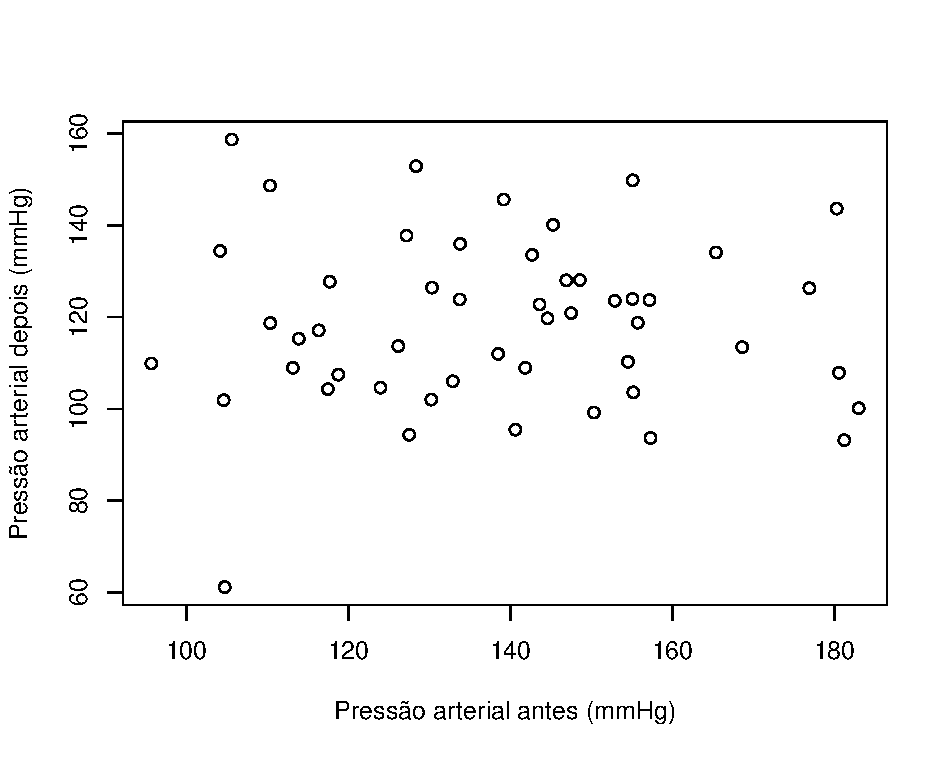
\includegraphics[scale=.5]{figures/blood_pressure.pdf}
 \end{center}
\end{figure}
\end{frame}

\begin{frame}{Teste t pareado: execução}
Estamos, portanto, interessados na hipótese\footnote{Note que, neste caso, esta é a hipótese razoável a ser testada, porque estamos interessados apenas em rejeitar a hipótese de que a droga~\textbf{não aumenta} a pressão arterial dos pacientes.
Drogas que não tem efeito ou causam aumento da pressão não costumam ser aprovadas pela ANVISA.}
\begin{align*}
   H_0 &: \mu_{\text{antes}} \leq \mu_{\text{depois}}, \\
   H_1 &:  \mu_{\text{antes}} > \mu_{\text{depois}}.
  \end{align*}

Podemos modelar a variável $Z_i = X_i-Y_i$ e sabemos que $Z_i \sim\operatorname{Normal}(\mu_Z = \mu_{\text{antes}}-\mu_{\text{depois}}, 2\sigma^2)$.
Desta forma, estamos interessados em testar hipóteses sobre $\mu_Z$ a partir de $\boldsymbol{Z}$.
Em particular, a hipótese acima se traduz em
\begin{align*}
   H_0 &: \mu_Z \leq 0, \\
   H_1 &: \mu_Z > 0,
\end{align*}
uma hipótese que podemos testar utilizando um teste t unicaudal como já discutido.
\end{frame}

\begin{frame}{Teste t para duas amostras}
Considere agora a situação em que dispomos de dois conjuntos de dados, $\boldsymbol{X} = \{X_1, X_2, \ldots, X_m\}$ e $\boldsymbol{Y} = \{Y_1, Y_2, \ldots, Y_n\}$ e queremos estudar diferenças nas médias.
Novamente, vamos modelar os processos como distribuições normais: $X_i \sim\operatorname{Normal}(\mu_1, \sigma_1^2), i = 1, 2, \ldots, m$ e $Y_j \sim\operatorname{Normal}(\mu_2, \sigma_2^2), j = 1, 2, \ldots, n$.

Sob a premissa de homogeneidade $\sigma_1^2 = \sigma_2^2 = \sigma^2$, podemos testar a hipótese
\begin{align*}
   H_0 &: \mu_1 \leq \mu_2, \\
   H_1 &: \mu_1 > \mu_2,
\end{align*}
computando a estatística 
\begin{equation*}
 U = \frac{\sqrt{m + n - 2}(\bar{X}_m - \bar{Y}_n)}{\sqrt{\left(\frac{1}{m} + \frac{1}{n}\right) (S_X^2 + S_Y^2)}},
\end{equation*}
onde $\bar{X}_m = (1/m)\sum_{i=1}^m X_i$,  $\bar{Y}_n = (1/n)\sum_{j=1}^n Y_j$, $S_X^2 = \sum_{i=1}^m (X_i-\bar{X}_m)^2$ e $S_Y^2 = \sum_{j=1}^n (Y_j-\bar{Y}_n)^2$.
\textbf{O teste procede analogamente ao que já foi discutido}.
\end{frame}

\begin{frame}{Relaxando a premissa de homogeneidade}
Até aqui assumimos variâncias iguais, tanto no teste pareado quanto no teste para duas amostras. 
Podemos relaxar a premissa de igualdade das variâncias um pouco se assumirmos que $\sigma_2^2 = k\sigma_1^2$, isto é, que a razão entre as variâncias é conhecida.
Neste caso, a estatística teste vale
\begin{equation*}
 U_k = \frac{\sqrt{m + n - 2}(\bar{X}_m - \bar{Y}_n)}{\sqrt{\left(\frac{1}{m} + \frac{k}{n}\right) (S_X^2 + \frac{S_Y^2}{k})}}.
\end{equation*}

Quando as variâncias são diferentes e desconhecidas e não conhecemos $k$, temos o problema de Behrens-Fisher\footnote{Em homenagem ao químico alemão Walter-Ulrich Behrens (1902--1962) e ao biólogo e estatístico britânico Ronald Aylmer Fisher (1890-1962).} que é muito mais difícil de tratar.
\end{frame}

\begin{frame}{O teste t bicaudal (bilateral)}
No caso do  teste t pareado, podemos estar interessados apenas em testar $\mu_{\text{antes}}= \mu_{\text{depois}}$, o que levaria a uma hipótese alternativa composta e um teste bicaudal (bilateral).
Situação parecida acontece no caso de duas amostras quando queremos testar $\mu_1 = \mu_2$.
Nesses casos, podemos facilmente adaptar os testes discutidos para acomodar a hipótese bilateral.
Em ambos os casos, podemos fazer o teste ``rejeite $H_0$ se $|U|\geq T^{-1}(1-\alpha_0/2; n-1)$'', e este terá tamanho $\alpha_0$.
\begin{figure}
 \begin{center}
  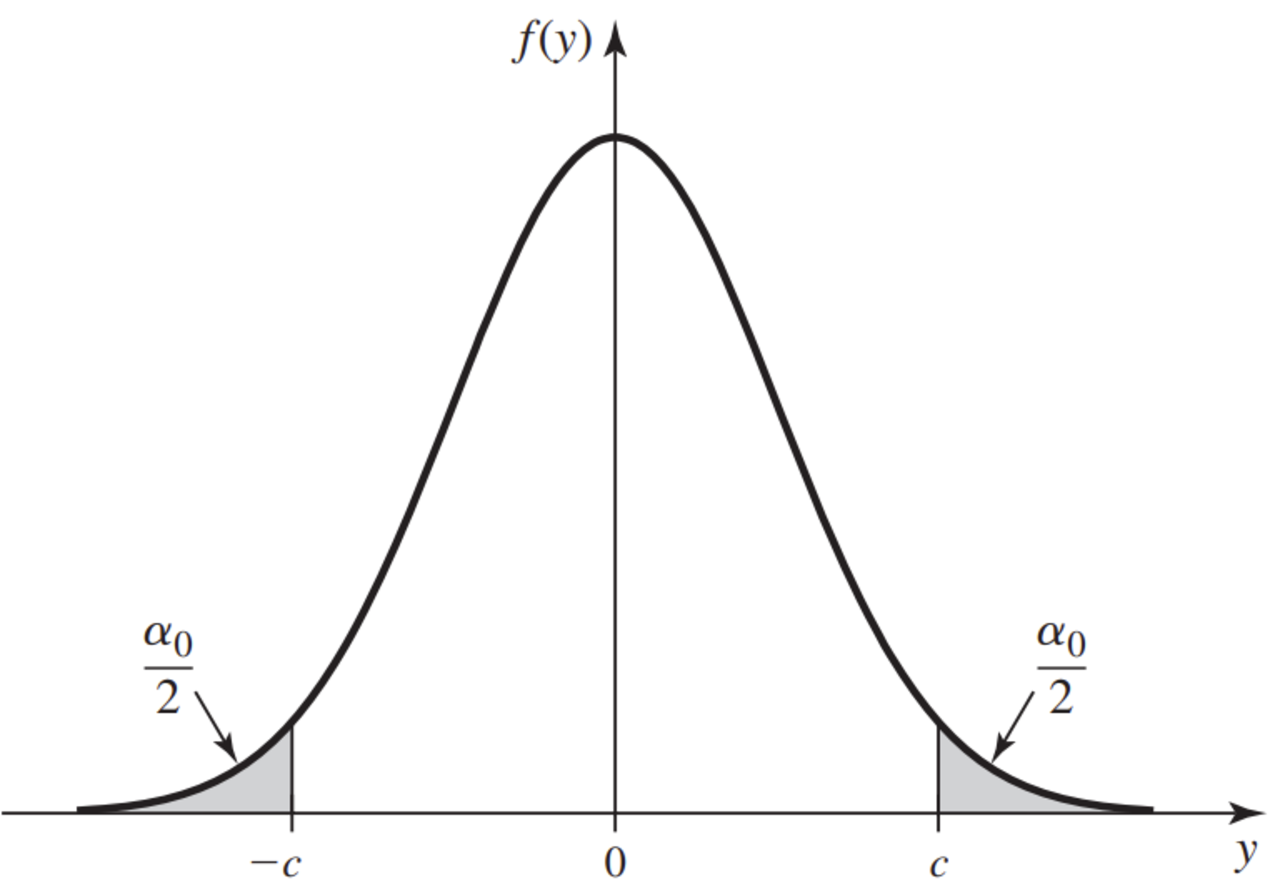
\includegraphics[scale=0.3]{figures/bilateral.pdf}
 \end{center}
\end{figure}
\end{frame}

\begin{frame}{O Teste t como um TRV (LRT)}
Podemos também entender o teste t como um teste de razão de verossimilhanças.
Em particular, temos para um teste t unicaudal, 
\begin{align*}
 \Lambda(\bx) &= \frac{\sup_{(\mu, \sigma^2):\mu > \mu_0} f_n(\bx \mid \mu, \sigma^2) }{\sup_{(\mu, \sigma^2)} f_n(\bx \mid \mu, \sigma^2)}, \\
 &=  \begin{cases}
     \left(\frac{\hat{\sigma^2}}{\hat{\sigma_0^2}}\right)^{n/2} \: \text{se} \: \sm> \mu_0,\\
     1,\:\text{caso contrário},
\end{cases} 
\end{align*}
onde $\hat{\sigma^2}$ é o EMV da variância e $\hat{\sigma_0^2} = \frac{1}{n}\sum_{i=1}^n (x_i-\mu_0)^2$.
Onde o teste t tradicional rejeita $H_0$ se $U\geq c$, sua formulação TRV rejeita $H_0$ se $\Lambda(\bx) \leq k$.
A relação entre $c$ e $k$ é 
\begin{equation*}
 c = \sqrt{\left[\left(\frac{1}{k^2}\right)^{1/n} - 1 \right](n-1)}, 
\end{equation*}
o que estabelece que o teste t é um teste de razão de verossimilhanças.
\end{frame}

\begin{frame}{O que aprendemos?}
\begin{itemize}
  \item[\faLightbulbO] O teste t permite comparar a média de um conjunto de dados com um valor postulado $\mu_0$;    
  \item[\faLightbulbO] Permite também comparar as médias de duas amostras, pareadas ou independentes;
  \item O teste t é não-viesado e pode ser escrito como um teste de razão de verossimilhanças;
   \end{itemize}
 \end{frame}

\begin{frame}{Leitura recomendada}
\begin{itemize}
 \item[\faBook] DeGroot seções 9.5 e 9.6;
 \item[\faBook] $^\ast$ Casella \& Berger (2002), seção 8.
 \item[\faForward] Próxima aula: DeGroot, seção 9.7;
 \item {\large\textbf{Exercícios recomendados}}
  \begin{itemize}
   \item[\faBookmark] DeGroot Seção 9.5: exercício 8.
  \end{itemize}
 \end{itemize} 
\end{frame}

\section{Testes para igualdade de variâncias}
\begin{frame}{Testes para igualdade de variâncias}
 \begin{itemize}
   \item A distribuição F;
   \item Comparação de variâncias de duas normais;
   \item Propriedades; 
   \item P-valor;
   \end{itemize}
\end{frame}


 \begin{frame}{A distribuição F}
  Sejam $Y \sim\operatorname{Qui-quadrado}(m)$ e $W \sim\operatorname{Qui-quadrado}(n)$.
  Então 
  \begin{equation*}
   X = \frac{Y/m}{W/n},
  \end{equation*}
tem distribuição $F$ com $m$ e $n$ graus de liberdade, com f.d.p.
\begin{equation*}
 f_X(x) = \frac{\Gamma\left(\frac{m + n}{2}\right)m^{m/2} n^{n/2}}{\Gamma\left(\frac{n}{2}\right)\Gamma\left(\frac{m}{2}\right)} \cdot \frac{x^{m/2}-1}{(mx + n)^(m + n)/2}, \: x > 0.
\end{equation*}
\begin{theo}[Propriedades da distribuição F]
 \begin{itemize}
  \item[i)] Se $X \sim F(m, n)$, então $\frac{1}{X} \sim F(n, m)$;
  \item[ii)] Se $Y \sim\operatorname{Student}(n)$, então $Y^2 \sim F(1, n)$.
 \end{itemize}
\end{theo}
\textbf{Prova:} Transformação de v.a.s padrão.
Exercício para a leitora.
 \end{frame}

 \begin{frame}{Testando a igualdade de duas variâncias}
  Suponha $X_i \sim\operatorname{Normal}(\mu_1, \sigma_1^2), i = 1, 2, \ldots, m$ e $Y_j \sim\operatorname{Normal}(\mu_2, \sigma_2^2), j = 1, 2, \ldots, n$.
  Estamos interessados em testar
  \begin{align*}
   H_0 &: \sigma_1^2 \leq \sigma_2^2 , \\
   H_1&:  \sigma_1^2 > \sigma_2^2. 
  \end{align*}
 Para isso, vamos computar a estatística de teste 
 \begin{equation*}
  V = \frac{S_X^2/(m-1)}{S_Y^2/(n-1)},
 \end{equation*}
 onde $S_X^2 = \sum_{i=1}^m (X_i-\bar{X}_m)^2$ e $S_Y^2 = \sum_{j=1}^n (Y_j-\bar{Y}_n)^2$.
 
 \begin{defn}[O teste F]
 \label{def:F_test}
  O teste F de homogeneidade (igualdade de variâncias)  é o teste $\delta_c$ que rejeita $H_0$ se $V \geq c$, para uma constante positiva $c$.
 \end{defn}

 \end{frame}

 \begin{frame}{Propriedades do teste F}
  Em primeiro lugar, podemos fazer afirmações sobre a distribuição de (uma transformação de) $V$.
  \begin{theo}[A distribuição de $V$]
   Seja $V = \frac{S_X^2/(m-1)}{S_Y^2/(n-1)}$, então:
   \begin{equation*}
    \frac{\sigma_2^2}{\sigma_1^2} V \sim F(m-1, n-1).
   \end{equation*}
   Além disso, se $\sigma_1^2 = \sigma_2^2$, $V \sim F(m-1, n-1)$. 
  \end{theo}
\textbf{Prova:} Notar que $S_X^2/\sigma_1^2$ e $S_Y^2/\sigma_2^2$  tem distribuição qui-quadrado com $m-1$ e $n-1$ graus de liberdade, respectivamente.
Ver Teorema 9.7.3 de DeGroot.
 \end{frame}
 
 \begin{frame}{P-valor}
  Seja $G(x; m-1, n-1)$ a f.d.a. de uma distribuição $F$ com $m-1$ e $n-1$ graus de liberdade.
  Da mesma forma, defina $G^{-1}(p; m-1, n-1)$ como a f.d.a. inversa.
  Então, se $V = v$:
  \begin{itemize}
   \item Para a hipótese $H_0: \sigma_1^2 \leq \sigma_2^2$, o p-valor vale $p = 1-G(v; m-1, n-1)$;
   \item Para a hipótese $H_0: \sigma_1^2 \geq \sigma_2^2$, o p-valor vale $p = G(v; m-1, n-1)$;
   \item Para a hipótese bicaudal $H_0: \sigma_1^2 \neq \sigma_2^2$, o p-valor vale $p = 2\min\left\{1-G(v; m-1, n-1), G(v; m-1, n-1)\right\}$;
  \end{itemize}
 \end{frame}
 
  \begin{frame}{Mais propriedades do teste F}
 Analogamente ao teste t, podemos enunciar o seguinte teorema sobre o teste F.
 \begin{theo}[Propriedades do teste F]
 Suponha que estamos testando $H_0: \sigma_1^2 \leq \sigma_2^2$.
 Então
 \begin{itemize}
 \item [i)] $\pi(\mu_1, \mu_2, \sigma_1^2, \sigma_2 \mid \delta_c) = 1 -G\left(\frac{\sigma_2^2}{\sigma_1^2}c; m-1, n-1\right)$;
 \item [ii)] $\sigma_1^2 = \sigma_2^2 \implies \pi(\mu_1, \mu_2, \sigma_1^2, \sigma_2 \mid \delta_c) = \alpha_0$;
 \item [iii)] $\sigma_1^2 < \sigma_2^2 \implies \pi(\mu_1, \mu_2, \sigma_1^2, \sigma_2 \mid \delta_c) < \alpha_0$
 \item [iv)] $\sigma_1^2 > \sigma_2^2 \implies \pi(\mu_1, \mu_2, \sigma_1^2, \sigma_2 \mid \delta_c) > \alpha_0$;
 \item [v)] $\lim_{\sigma_1/\sigma_2 \to 0} \pi(\mu_1, \mu_2, \sigma_1^2, \sigma_2 \mid \delta_c) = 0$;
 \item [vi)] $\lim_{\sigma_1/\sigma_2 \to \infty} \pi(\mu_1, \mu_2, \sigma_1^2, \sigma_2 \mid \delta_c) = 1$;
 \item[vii)] $\delta_c$ é não-viesado e tem tamanho $\alpha_0$.
\end{itemize}
\end{theo}
\textbf{Prova:} Omitida aqui. 
Ver Teorema 9.7.4 de DeGroot.  
 \end{frame}
 
\begin{frame}{O que aprendemos?}
\begin{itemize}
  \item[\faLightbulbO] A distribuição F aparece quando tomamos a razão de variáveis aleatórias Qui-quadrado;    
  \item[\faLightbulbO] Para comparação das variâncias de duas amostras a estatística teste tem distribuição $F$ com $m-1$ e $n-1$ graus de liberdade; 
  \item O teste F, como seu primo o teste t, é não viesado e tem tamanho $\alpha_0$.
   \end{itemize}
 \end{frame} 
 
\begin{frame}{Leitura recomendada}
\begin{itemize}
 \item[\faBook] DeGroot seção 9.7;
 \item[\faBook] $^\ast$ Casella \& Berger (2002), seção 8.
 \item[\faForward] Próxima aula: De Groot, seção 11;
 \item {\large\textbf{Exercícios recomendados}}
  \begin{itemize}
   \item[\faBookmark] Derivar a função de densidade de probabilidade de uma distribuição F (Teorema 9.7.1 de DeGroot).
   \item[\faBookmark] Derivar o teste F como um teste de razão de verossimilhanças.
  \end{itemize}
 \end{itemize} 
\end{frame}

\section{Regressão linear}
\begin{frame}{Regressão linear}
 \begin{itemize}
   \item Mínimos quadrados;
   \item Modelo de regressão simples (univariado);
   \begin{itemize}
    \item Formulação;
    \item Premissas.
   \end{itemize}
   \item Distribuição amostral dos estimadores;    
   \item Intervalos de confiança para os coeficientes;
   \item Testes para os coeficientes;
   \item Predição: pontual e intervalar.
   \end{itemize}
\end{frame} 

\begin{frame}{Regressão linear: motivação}
 \begin{figure}
  \begin{center}
   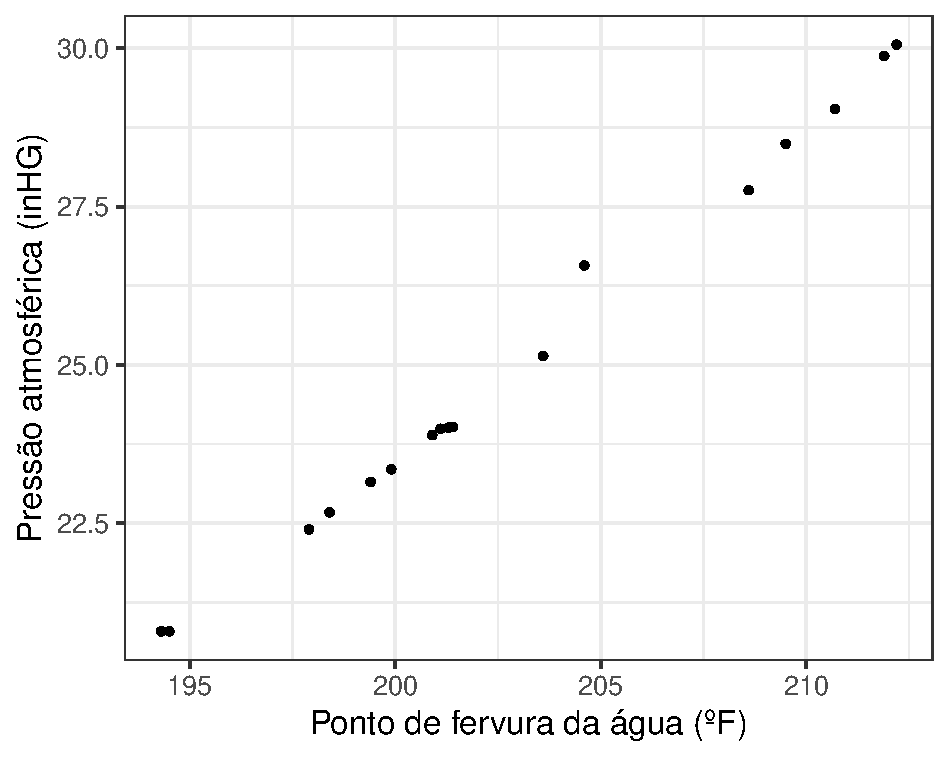
\includegraphics[scale=.6]{figures/pressure_data.pdf}
  \end{center}
 \end{figure}
\end{frame}

\begin{frame}{Mínimos quadrados}
Suponha que estamos interessados na reta 
\begin{equation}
 \label{eq:line}
 y_i = \beta_0  + \beta_1x_i.
\end{equation}
\begin{itemize}
 \item $\beta_0$ é chamado o~\textbf{intercepto} (\textit{intercept}) da reta;
 \item $\beta_1$ é chamado o~\textbf{coeficiente angular} (\textit{slope}) da reta.
\end{itemize}

\begin{theo}[A linha de mínimos quadrados]
\label{thm:least_squares_line}
 Sejam $(x_1, y_1), (x_2, y_2), \ldots, (x_n, y_n)$ uma coleção de $n$ pontos.
 Os valores dos coeficientes que minimizam a soma de quadrados são
 \begin{align*}
  \hat{\beta_0} &= \bar{y} - \hat{\beta_1}\bar{x},\\
  \hat{\beta_1} &= \frac{\sum_{i=1}^n (y_i-\bar{y})(x_i-\bar{x})}{\sum_{i=1}^n \left(x_i - \bar{x}\right)^2},
 \end{align*}
 onde $\bar{x} = (1/n)\sum_{i=1}^n x_i$ e $\bar{y} = (1/n)\sum_{i=1}^n y_i$.
\end{theo}
\textbf{Prova:} Escrever a equação de estimação,$Q = \sum_{i=1}^n \left(y_i - (\beta_0 + \beta_1x_i) \right)^2$, diferenciar $Q$ com respeito aos coeficientes e igualar a zero. 
Ver Teorema 11.1.1 em DeGroot.
\end{frame}

\begin{frame}{O modelo linear}
 Podemos construir um modelo estatístico explícito para a relação entre as variáveis\footnote{Em notação de matrizes,$E[Y] = \bX^T\boldsymbol{\beta}$.} $\bX$ e $Y$:
 \begin{equation}
  \label{eq:lin_mod}
  E[Y \mid \bX = x_1, x_2, \ldots, x_P] = \beta_0 + \beta_1x_1 + \beta_2x_2 + \ldots + \beta_Px_P.  
 \end{equation}
\textbf{Terminologia:}
\begin{itemize}
\item $Y$ é chamada de desfecho,~\textbf{variável-resposta} ou variável dependente;
\item $\bX$ são chamados covariáveis,~\textbf{preditores} ou, ainda, variáveis independentes;
\item $\boldsymbol{\beta} = \{\beta_0, \beta_1, \ldots, \beta_P\}$ são os~\textbf{coeficientes de regressão}.
\end{itemize}

Podemos então idealizar o seguinte modelo
\begin{ideia}[Modelo linear]
 \[ Y_i = \beta_0 + \sum_{j=1}^P \beta_jx_{ij} + \epsilon_i,\: \epsilon_i \sim\operatorname{Normal}(0, \sigma^2).\]
\end{ideia}
\end{frame}

\begin{frame}{Premissas (importante!)}
Como todo modelo, a regressão linear se apoia em premissas sobre os dados e o seu processo gerador.
\begin{itemize}
 \item[P1.] O(s) preditor(es) é (são) conhecido(s);
 \item[P2.] Normalidade: dados os preditores $\bX$, a resposta $Y$ tem distribuição normal;
 \item[P3.] Linearidade na média: a esperança condicional de $Y$ é dada por $\beta_0 + \sum_{j=1}^P \beta_jx_{ij}$;
 \item[P4.] Variância comum (\textbf{homocedasticidade}): a variância condicional de $Y_i$ é  $\sigma^2$ para todo $i = 1, 2, \ldots, n$;
 \item[P5.] Independência (condicional): dados os valores de $\bX$, os valores de $Y$ são idependentes entre si.
\end{itemize}
\end{frame}

\begin{frame}{Cuidado! Quarteto de Anscombe\footnote{Em homenagem ao estatístico Britânico Francis Anscombe (1918-2001).}}
  \begin{figure}
  \begin{center}
   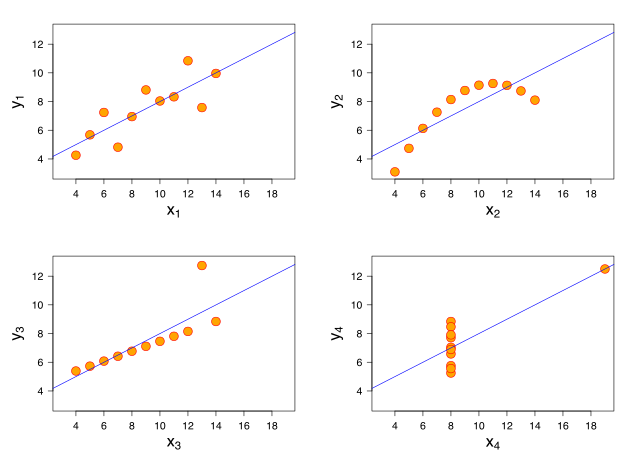
\includegraphics[scale=.435]{figures/anscombe.png}
  \end{center}
  \label{fig:anscombe_quartet}
 \end{figure}
\end{frame}

\begin{frame}{Um teorema interessante}
No modelo linear, a solução de mínimos quadrados e a de máxima verossimilhança coincidem!
\begin{theo}[EMV para os coeficientes de uma regressão linear (simples)]
\label{thm:MLE_linreg_coefficients}
 Sob as premissas já listadas, os estimadores de máxima verossimilhança para $\theta = (\beta_0, \beta_1, \sigma^2)$ são
  \begin{align*}
  \hat{\beta_0}_{\text{EMV}} &= \bar{y} - \hat{\beta_1}_{\text{EMV}}\bar{x},\\
  \hat{\beta_1}_{\text{EMV}} &= \frac{\sum_{i=1}^n (y_i-\bar{y})(x_i-\bar{x})}{\sum_{i=1}^n \left(x_i - \bar{x}\right)^2},\\
  \hat{\sigma^2}_{\text{EMV}} & = \frac{1}{n} \sum_{i=1}^n \left(y_i - (  \hat{\beta_0}_{\text{EMV}} + \hat{\beta_1}_{\text{EMV}} x_i)\right)^2,  
 \end{align*}
 ou seja, os estimadores de máxima verossimilhança dos coeficientes minimizam a soma de quadrados da reta estimada.
\end{theo}
\textbf{Prova:} Ver Teorema 11.2.1 de DeGroot.
\end{frame}

\begin{frame}{Distribuição amostral dos estimadores}
Sob as premissas já discutidas, podemos fazer afirmações sobre a distribuição amostral dos estimadores obtidos:
\begin{theo}[Distribuição amostral dos estimadores dos coeficientes]
\label{thm:sampling_distribution_linreg_coefficients}
   \begin{align*}
  \hat{\beta_0}_{\text{EMV}} &\sim \operatorname{Normal}\left(\beta_0, \sigma^2 \left( \frac{1}{n} + \frac{\bar{x}^2}{s_x^2} \right) \right),\\
  \hat{\beta_1}_{\text{EMV}}  &\sim \operatorname{Normal}\left(\beta_1, \frac{\sigma^2}{s_x^2}\right),\\
  &\operatorname{Cov}\left(\hat{\beta_0}_{\text{EMV}}, \hat{\beta_1}_{\text{EMV}} \right)  = -\frac{\bar{x}\sigma^2}{s_x^2},
 \end{align*}
 onde $s_x = \sqrt{\sum_{i=1}^n (x_i-\bar{x})^2}$.
\end{theo}
\textbf{Prova:} Usar as leis de esperanças e variâncias.
Ver Teorema 11.2.2 de DeGroot.
\end{frame}

\begin{frame}{Intervalos de confiança para os coeficientes}
Podemos computar intervalos de confiança para os coeficientes da regressão linear de maneira muito similar ao que já vimos para o caso da média da Normal.

\begin{theo}[Intervalos de confiança para os coeficientes de uma regressão linear]
\label{thm:CIs_linreg_coefficients}
\begin{align*}
 &\hat{\beta_0} \pm \hat{\sigma}^\prime c\sqrt{\frac{1}{n} + \frac{\bar{x}^2}{s_x^2}}\quad \text{e}\quad \hat{\beta_1} \pm c\frac{\hat{\sigma}^\prime}{s_x},\\
 &\hat{\beta_0} + \hat{\beta_1}x_{\text{pred}} \pm c \hat{\sigma}^\prime \sqrt{\frac{1}{n} + \frac{\left(x_{\text{pred}}-\bar{x}\right)^2}{s_x^2} },
\end{align*}
onde $c = T^{-1}(1-\frac{\alpha_0}{2}; n-2)$ e 
\begin{equation*}
 \hat{\sigma}^\prime := \sqrt{\frac{\sum_{i=1}^n \left(Y_i - \hat{\beta_0} - \hat{\beta_1}x_i \right)^2}{n-2}}.
\end{equation*}
\end{theo}
\textbf{Prova:} Usar o Teorema 11.3.5 de DeGroot e os valores apropriados de $c_0$ e $c_1$.
\end{frame}

\begin{frame}{Testes de hipóteses para o coeficiente angular}
Em geral, estamos interessados em testar a hipótese
\begin{align*}
 H_0 &: \beta_1 = \beta^\star,\\
 H_1 &: \beta_1 \neq \beta^\star.
\end{align*}
Para tanto, podemos computar a estatística
\begin{equation*}
 U_1 = s_x \frac{\hat{\beta_1}-\beta^\star}{\hat{\sigma}^\prime},
\end{equation*}
e computar o p-valor como 
\begin{equation*}
 \pr(U_1 \geq |u_1|) + \pr(U_1 \leq -|u_1|).
\end{equation*}
Notando que $U_1$ tem distribuição t de Student com $n-2$ graus de liberdade sob $H_0$, podemos computar o p-valor exatamente.

Resultados bem similares valem para testar hipóteses sobre $\beta_0$ ou $\hat{Y}$.
\end{frame}

\begin{frame}{Predição pontual}
Suponha que queremos prever o valor de $Y$ para um certo $x_{\text{pred}}$ que não foi observado no experimento.
Podemos compor nossa predição (pontual) como 
\begin{equation}
 \label{eq:lin_pred}
\hat{Y} = \hat{\beta_0} + \hat{\beta_1}x_{\text{pred}}. 
\end{equation}

\begin{theo}[Erro quadrático médio da predição]
\label{thm:MSE_linreg_pred}
 A predição como em~(\ref{eq:lin_pred}) tem erro quadrático médio (EQM) igual a
 \[ E\left[\left(\hat{Y} - Y\right)^2\right] = \sigma^2 \left(1 + \frac{1}{n} + \frac{\left(x_{\text{pred}}-\bar{x}\right)^2}{s_x^2}\right). \] 
\end{theo}
\textbf{Prova:} Ver Teorema 11.2.3 de DeGroot.

\begin{obs}[EQM fora da amostra]
 O EQM aumenta quanto mais longe $x_{\text{pred}}$ estiver dos valores de $X$ que foram medidos (observados).
\end{obs}
\end{frame}

\begin{frame}{Predição intervalar}
Muitas vezes estamos interessados em produzir um~\textit{intervalo} para a nossa predição, ao invés de um único valor (predição pontual). 
Nesta situação, podemos fazer uso do seguinte teorema:
\begin{theo}[Intervalos de \textbf{predição} para $\hat{Y}$]
\label{thm:CI_pred_mean}
A probabilidade de $\hat{Y} = \hat{\beta_0} + \hat{\beta_1}x_{\text{pred}}$ estar no intervalo
\begin{equation*}
 \hat{Y} \pm T^{-1}\left(1-\frac{\alpha_0}{2}; n-2\right)\hat{\sigma}^\prime \sqrt{\left[ 1+ \frac{1}{n} + \frac{\left(x_{\text{pred}}-\bar{x}\right)^2}{s_x^2} \right]},
\end{equation*}
é $1-\alpha_0$.
\end{theo}
\textbf{Prova:} Ver Teorema 11.3.6 de DeGroot.
\end{frame}

\begin{frame}{Intervalos de confiança e de predição: ilustração}
 \begin{figure}
  \begin{center}
   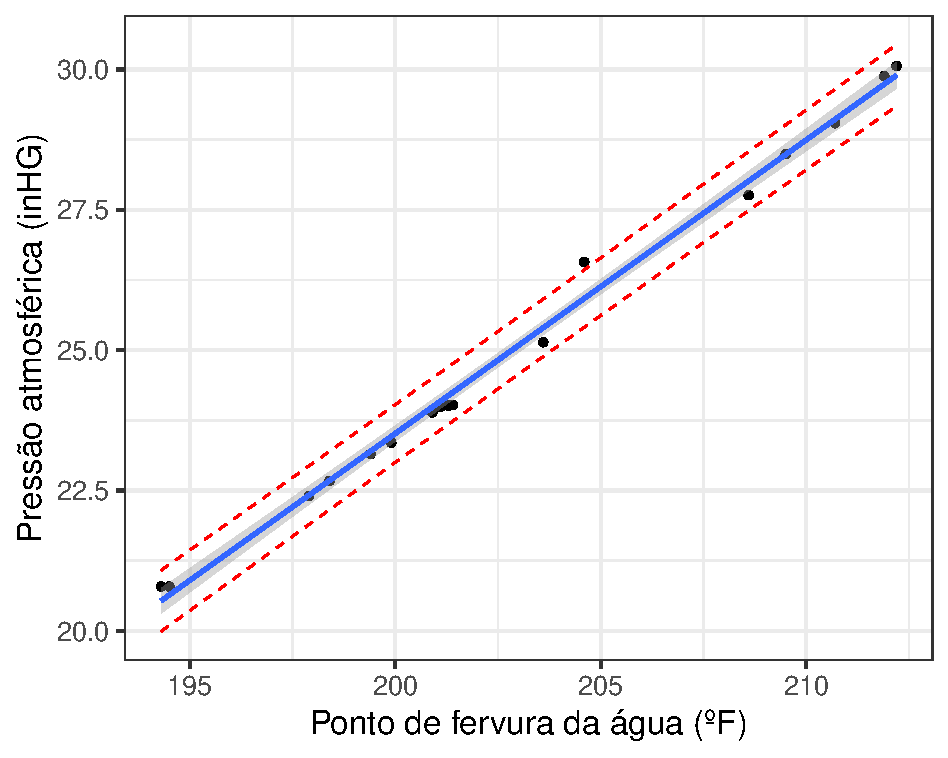
\includegraphics[scale=.6]{figures/pressure_model.pdf}
  \end{center}
 \end{figure}
\end{frame}

\begin{frame}{O que aprendemos?}
\begin{itemize}
  \item[\faLightbulbO] O modelo linear permite modelar a relação (linear) entre uma (ou mais) variável(is) independente(s) e uma variável dependente;    
  \item[\faLightbulbO] A estimação dos coeficientes pode ser feita por mínimos quadrados; 
  \item[\faLightbulbO] A solução de mínimos quadrados é também a solução de máxima verossimilhança!
  \item[\faLightbulbO] Podemos aplicar a teoria Normal para testar hipóteses sobre os coeficientes e calcular intervalos de confiança;
  \item[\faLightbulbO] Podemos produzir predições sobre a variável dependente para valores não-observados da(s) variável(is) independente(s).
   \end{itemize}
 \end{frame} 
 
\begin{frame}{Leitura recomendada}
\begin{itemize}
 \item[\faBook] DeGroot seções 11.1, 11.2 e 11.3;
 \item[\faBook] $^\ast$ Casella \& Berger (2002), seção 11.3.
 \item[\faForward] Próxima aula: DeGroot, seção 9.9;
 \item {\large\textbf{Exercícios recomendados}}
  \begin{itemize}
   \item[\faBookmark] DeGroot, seção 11.1: exercício 3.
   \item[\faBookmark] DeGroot, seção 11.2: exercícios 2, 3 e 6.
   \item[\faBookmark] $^\ast$ Bônus: DeGroot, seção 11.2: exercício  19 (valendo 0.5 na média).
  \end{itemize}
 \end{itemize} 
\end{frame}

\section{Discussão de TSHN}
\begin{frame}{Testes de hipótese: discussão}
 \begin{itemize}
 \item Como construir um teste que~\textbf{quase sempre} rejeita $H_0$;
 \item Significância estatística~\textit{vs} significância prática;
 \item Rapidinhas.
 \end{itemize}
\end{frame} 

\begin{frame}{Um teste esquisito}

Suponha que temos $\rs$ vindos de uma distribuição Normal com média $\theta$ e variância $1$ e queremos testar as hipóteses
\begin{align*}
 H_0:& \theta = 0,\\
 H_1:& \theta = 1.
\end{align*}
Seguindo o exemplo 9.2.5 de DeGroot, podemos escrever
\begin{equation*}
 \eta(\bx) = \frac{f_1(\bx)}{f_0(\bx)},
\end{equation*}
e compor um teste que rejeita $H_0$ quando $\eta(\bx) > c$.
Isto é equivalente a construir um teste de tamanho $\alpha_0$, de modo que valha
\begin{equation*}
 \pr(\Sm \geq c^\prime \mid \theta = 0) = \alpha_0,
\end{equation*}
o que nos leva a concluir que $c^\prime = \frac{1}{2} + \frac{\log(c)}{n}$ e que $c = \Phi^{-1}(1-\alpha_0)/\sqrt{n}$.
\end{frame}

\begin{frame}{Qual o problema?}
Primeiro, vamos lembrar que, para um teste $\delta$, 
\begin{align*}
 \alpha(\delta)&:= \pr\left(\text{Rejeitar\:} H_0 \mid \theta = 0\right) ,\\
 \beta(\delta)&:= \pr\left(\text{Não\, rejeitar\:} H_0 \mid \theta = 1\right).
\end{align*}

 O problema aqui é que para este teste temos
 \begin{table}
  \begin{tabular}{cccc}
   n & $\alpha(\delta)$ & $\beta(\delta)$ & c \\
   \hline
   1 & 0.05 & 0.74 & 0.72 \\
   25 & 0.05 & 3.97 $\times 10^{-4}$  & 2.3 $\times 10^{-4}$ \\
   100 & 0.05 &  8 $\times 10^{-15}$ & 2.7 $\times 10^{-15}$\\
   \hline
  \end{tabular}
 \end{table}
Ou seja, quando temos $n=100$ observações, os dados podem ser trilhões de vezes mais prováveis sob $H_0$ e ainda assim vamos rejeitar a hipótese nula.
\end{frame}

\begin{frame}{Soluções}
 Podemos pensar em duas soluções (complementares) para o problema posto.
\begin{ideia}[Ajustando o nível de significância com o tamanho da amostra]
 Em várias situações, por exemplo como a mostrada acima, faz sentido ajustar (diminuir) o nível de confiança do teste com o tamanho da amostra de modo a balancear os erros do tipo I e II.
\end{ideia}

\begin{ideia}[Minimizar uma combinação linear das probabilidades de erro]
Poderíamos balancear os erros ao minimizar
\[ a \alpha(\delta) + b \beta(\delta). \]
Lehmann (1958)\footnote{Lehmann, Erich L. "Significance level and power." The Annals of Mathematical Statistics (1958): 1167-1176.} propôs a restrição $\beta(\delta) = c \alpha(\delta)$, que tem a vantagem de forçar que ambos os tipos de erro diminuam à medida que obtemos mais dados.
\end{ideia}
Ver seções 9.2 e 9.8 de DeGroot.
\end{frame}

\begin{frame}{Relevante?}
 Suponha que eu estou testando uma nova droga, e o parâmetro $\theta$ mede o efeito da droga.
 Em geral, estamos interessados em testar a hipótese
 \begin{align*}
 H_0: \theta \leq 0,\\
 H_1: \theta \geq  0.
 \end{align*}
Quando o tamanho de amostra é muito grande, seremos capazes de detectar, com alta probabilidade (poder) se $\theta = 0.000003$ ou $\theta = 0$.

Acontece que uma droga com $\theta = 0.000003$ não oferece nenhuma vantagem prática.
Portanto, ao se realizar um teste de hipótese e rejeitar $H_0$, não podemos concluir que ``a droga funciona'', pelo menos não num sentido médico.
\begin{ideia}[Significância estatística não implica relevância prática]
 \end{ideia}
\end{frame}

\begin{frame}{Responda rápido}
   \begin{itemize}
    \item[a)] O que é a função poder de um teste de hipótese e o que esperamos observar em um teste não-enviesado?
    \item[b)] Se testarmos uma hipótese um número suficiente de vezes ela eventualmente será rejeitada.
    Explique esta afirmação e suas consequências.
    \item[c)] O que é o p-valor de um teste?
    \item[d)] É correto afirmar que uma hipótese nula é falsa se ela for rejeitada?
    É correto afirmar que uma hipótese alternativa é verdadeira se a nula for rejeitada? Justifique.
    \item[e)] Um intervalo de confiança nível de 95\% para $\theta$ é calculado a partir de $n$ observações.
    É correto afirmar que o parâmetro verdadeiro $\theta_0$ está dentro deste intervalo com probabilidade $95\%$? Justifique.
    \item[f)] Explique como podemos obter um conjunto de confiança a partir de um teste de hipótese.
  \end{itemize}
\end{frame}


\begin{frame}{O que aprendemos?}
\begin{itemize}
  \item[\faLightbulbO] Rejeição eventual;
  ``Se coletarmos uma quantidade suficiente de dados, podemos rejeitar qualquer hipótese nula''
  \item[\faLightbulbO] Significância estatística $\neq$ significância prática/científica!
   \end{itemize}
 \end{frame} 
 
\begin{frame}{Leitura recomendada}
\begin{itemize}
 \item[\faBook] DeGroot seções 9.2, 9.3 e 9.9;
%  \item[\faBook] $^\ast$ Casella \& Berger (2002), seção 11.3.
   \item {\large\textbf{Exercícios recomendados}}
  \begin{itemize}
   \item[\faBookmark] DeGroot, seção 9.9: exercícios 2 e 3.   
  \end{itemize}
  \end{itemize}
\end{frame}

\end{document}
